\documentclass[a4paper,10pt]{article}
\usepackage[utf8]{inputenc}
\usepackage{amsmath}
\usepackage{amssymb}
\usepackage{amsfonts}
\usepackage{subfloat}
\usepackage{algorithm}
\usepackage{algpseudocode}
\usepackage{placeins}

\usepackage{color}
\definecolor{linkcol}{rgb}{0,0,0.4}
\definecolor{citecol}{rgb}{0.5,0,0}

\usepackage[pagebackref,hyperindex=true]{hyperref}
\hypersetup{colorlinks=true,linkcolor=linkcol,citecolor=citecol,urlcolor=linkcol}

\usepackage[version=3]{mhchem}

\usepackage{amsmath}
\usepackage{amssymb}
\usepackage{amsfonts}
\usepackage{amsopn}
\usepackage{braket}
\usepackage{bbm}
\usepackage{dsfont}
\usepackage{kpfonts}
% \usepackage{mathabx}

\parindent=0cm


% Various new commands that ease typesetting math even further
% \newcommand{\assign}{\ensuremath{\coloneq}}
% \newcommand{\rassign}{\ensuremath{\eqcolon}}
\newcommand{\assign}{\ensuremath{:=}}
\newcommand{\rassign}{\ensuremath{=:}}

\newcommand{\of}[1]{\ensuremath{\left( #1 \right)}}
\newcommand{\ofs}[1]{\ensuremath{\left( #1 \right)}}

\newcommand{\norm}[1]{\ensuremath{\| #1 \|}}

\newcommand{\tmop}[1]{\ensuremath{\operatorname{#1}}}

\newcommand{\id}{\ensuremath{\mathds{1}}}
% \newcommand{\id}{\ensuremath{I}}


\newcommand{\conj}[1]{\ensuremath{\overline{#1}}}

\newcommand{\T}{\ensuremath{{}^{\textnormal{T}}}}
\newcommand{\herm}{\ensuremath{{}^{\textnormal{H}}}}

\newcommand{\ft}[1]{\ensuremath{\mathcal{F}\left(#1\right)}}
\newcommand{\ift}[1]{\ensuremath{\mathcal{F}^{-1}\left(#1\right)}}

\newcommand{\fft}[1]{\ensuremath{\mathtt{FFT}\left(#1\right)}}
\newcommand{\ifft}[1]{\ensuremath{\mathtt{IFFT}\left(#1\right)}}

\newcommand{\dotp}[2]{\ensuremath{\langle #1 , #2 \rangle}}

\newcommand{\bigO}[1]{\ensuremath{\mathcal{O}\left( #1 \right)}}

\newcommand{\mat}[1]{\ensuremath{\mathbf{#1}}}

% multi-indices
\newcommand{\mindex}[1]{\ensuremath{\underline{#1}}}

\newcommand{\laplace}{\ensuremath{\operatorname{\Delta}}}

% EOF

\usepackage{graphicx}
\usepackage{subcaption}
\usepackage{asymptote}
\usepackage{tikz}
\usetikzlibrary{shapes,arrows}



\synctex=1
\parindent 0pt

%opening
\title{Numerical Steepest Descent for Overlap Integrals of Semiclassical Wavepackets}
\author{R. Bourquin}

\begin{document}

\maketitle

\section{Introduction}


\marginpar{What is NSD?}
\marginpar{Why do we need it?}


Given functions $f(x_1, \ldots, x_n):\mathbb{R}^N\rightarrow\mathbb{R}$ and
$g(x_1, \ldots, x_n):\mathbb{R}^N\rightarrow\mathbb{C}$, compute the integral:

\begin{equation} \label{eq:hoi}
 I := \int_{-\infty}^{\infty} \cdots \int_{-\infty}^{\infty} f \exp(i \omega g) \, \mathrm{d}x_1 \cdots \mathrm{d}x_n
\end{equation}

This is a highly oscillatory integral. Usually we call $g$ the \emph{oscillator}
and $f$ the \emph{amplitude} or \emph{envelope}. For more details see the work
by Huybrechs and some others. The main technique is described in \cite{HV_hoq} for
the one-dimensional case and in \cite{HV_cub} for multivariate integrands.
Semi-infinite intervals are treated in \cite{H_nsd_sii}.

\marginpar{cite \cite{AH_cgq_it}}


\section{About semi-classical wavepackets}

\marginpar{Exact formula for 1D overlap integral (?)}
\marginpar{Transformation to NSD highly oscillatory integral}
\marginpar{Properties of $A$, sym + i sym}
\marginpar{Put this section at the end?}


In this section we look at the wavepackets involved in the computation
of overlap integrals. Semiclassical wavepackets are constructed from a
Groundstate
\begin{align*}
  \phi_{\vec{0}}\left(\vec{x}\right)
  =
  (\pi\varepsilon^2)^{-\frac{D}{4}} (\det\mat{Q})^{-\frac{1}{2}}
  \exp \left( \frac{\imath}{2\varepsilon^2}
  \dotp{(\vec{x}-\vec{q})}{\mat{P}\mat{Q}\inv(\vec{x}-\vec{q})}
  + \frac{\imath}{\varepsilon^2} \dotp{\vec{p}}{(\vec{x}-\vec{q})}
  \right)
\end{align*}
by raising and lowering operators $\mathcal{R}$ and $\mathcal{L}$
and in the multi-dimensional case counted by a multi-index
$\vec{k} \in \mathbb{N}_0^D$. There are the parameters for average
position $\vec{q} \in \mathbb{R}^D$ and momentum $\vec{p} \in \mathbb{R}^D$
and the parameters $\mat{Q} \in \mathbb{C}^{D \times D}$ and $\mat{P} \in \mathbb{C}^{D \times D}$
for position and momentum spread. These parameters are usually collected
in the set $\Pi \assign \{\vec{q}, \vec{p}, \mat{Q}, \mat{P}\}$.
Further there is the semiclassical scaling parameter $\varepsilon > 0$.
For many more details describing these wavepackets, see \cite{H_ladder_operators}
and \cite{B_master_thesis}.
What matters most here is, that each wavepacket $\phi$ is of the form:

\begin{equation}
  \phi(\vec{x}) \sim p\left(\vec{x}\right)\exp\left(\frac{i}{\varepsilon^2} g\left(\vec{x}\right)\right) \,.
\end{equation}

This form is sufficient for the steepest descent technique to be applicable.
Indeed, comparing to the integrand in \eqref{eq:oscillatory_integral},
we find that $\omega = \frac{1}{\varepsilon^2}$. The method becomes
better the smaller $\varepsilon$ is.
The actual oscillator $g$ is of the form:

\begin{equation}
  g\left(\vec{x}\right)
  \assign
  \frac{1}{2} \dotp{\vec{x}-\vec{q}}{\mat{P}\mat{Q}\inv \left(\vec{x}-\vec{q}\right)}
  +
  \dotp{\vec{p}}{\vec{x}-\vec{q}}
\end{equation}

Usually we are interested in integrals of the form $\dotp{\phi_k}{\phi_l}$.
In that case the integral is still of the same oscillatory structure:

\begin{equation}
\begin{split}
  \dotp{\phi_k}{\phi_l} & =
  \int_{-\infty}^{\infty} \conj{p_k(x)\exp\left(\frac{i}{\varepsilon^2} g_k(x)\right)}
                                p_l(x)\exp\left(\frac{i}{\varepsilon^2} g_l(x)\right)
  \mathrm{d}\vec{x} \\
  & =
  \int_{-\infty}^{\infty}
    \conj{p_k(x)} p_l(x)
    \exp\left(-\frac{i}{\varepsilon^2} \conj{g_k(x)} + \frac{i}{\varepsilon^2} g_l(x)\right)
  \mathrm{d}\vec{x} \\
  & =
  \int_{-\infty}^{\infty}
    \conj{p_k(x)} p_l(x)
    \exp\left(\frac{i}{\varepsilon^2}\left(-\conj{g_k(x)} + g_l(x)\right)\right)
  \mathrm{d}\vec{x} \,.
\end{split}
\end{equation}

The next step to take is to combine both oscillators $g_k$ and $g_l$ into a
single one such that we get back a formal expression like the one in
\eqref{eq:oscillatory_integral} we started with.


\subsection{Combining different oscillators}

Combining the two oscillators is actually a straight-forward computation,
however it is very error prone, big chances are that we miss a transpose
or conjugate somewhere. To simplify the notation define:

\begin{equation}
  \mat{\Gamma_i} \assign \mat{P_i}\mat{Q_i}\inv
\end{equation}

and start with computing $\conj{g_k}$:

\begin{equation}
\begin{split}
 \conj{g_k}
 & =
 \frac{1}{2}\conj{\dotp{\vec{x}-\vec{q_k}}{\mat{\Gamma_k} \left(\vec{x}-\vec{q_k}\right)}}
 +\conj{\dotp{\vec{p_k}}{\vec{x}-\vec{q_k}}} \\
 & =
 \frac{1}{2} \left(
                \conj{\dotp{\vec{x}}{\mat{\Gamma_k} \vec{x}}}
               -\conj{\dotp{\vec{x}}{\mat{\Gamma_k} \vec{q_k}}}
               -\conj{\dotp{\vec{q_k}}{\mat{\Gamma_k} \vec{x}}}
               +\conj{\dotp{\vec{q_k}}{\mat{\Gamma_k} \vec{q_k}}}
              \right)
 + \conj{\dotp{\vec{p_k}}{\vec{x}}}
 - \conj{\dotp{\vec{p_k}}{\vec{q_k}}} \\
 & =
 \frac{1}{2} \left(
               \vec{x}\H \mat{\Gamma_k}\H \vec{x}
              -\vec{q_k}\H \mat{\Gamma_k}\H \vec{x}
              -\vec{x}\H \mat{\Gamma_k}\H \vec{q_k}
              +\vec{q_k}\H \mat{\Gamma_k}\H \vec{q_k}
              \right)
 + \vec{x}\H \vec{p_k} - \vec{q_k}\H \vec{p_k} \,.
\end{split}
\end{equation}

Next we add $g_l$ and simplify the following expression:

\begin{equation}
\begin{split}
 -\conj{g_k} + g_l
 = &
 -\frac{1}{2} \left(
               \vec{x}\H \mat{\Gamma_k}\H \vec{x}
              -\vec{q_k}\H \mat{\Gamma_k}\H \vec{x}
              -\vec{x}\H \mat{\Gamma_k}\H \vec{q_k}
              +\vec{q_k}\H \mat{\Gamma_k}\H \vec{q_k}
              \right)
 - \left(\vec{x}\H \vec{p_k} - \vec{q_k}\H \vec{p_k}\right) \\
 & +
  \frac{1}{2} \left(
                \vec{x}\H \mat{\Gamma_l} \vec{x}
               -\vec{x}\H \mat{\Gamma_l} \vec{q_l}
               -\vec{q_l}\H \mat{\Gamma_l} \vec{x}
               +\vec{q_l}\H \mat{\Gamma_l} \vec{q_l}
              \right)
 + \left(\vec{p_l}\H \vec{x} - \vec{p_l}\H \vec{q_l}\right) \\
 = &
 \frac{1}{2} \left(\vec{x}\H \mat{\Gamma_l} \vec{x} - \vec{x}\H \mat{\Gamma_k}\H \vec{x}\right)
 +
 \frac{1}{2} \left(
               \vec{q_k}\H \mat{\Gamma_k}\H \vec{x}
              +\vec{x}\H \mat{\Gamma_k}\H \vec{q_k}
              -\vec{x}\H \mat{\Gamma_l} \vec{q_l}
              -\vec{q_l}\H \mat{\Gamma_l} \vec{x}
             \right) \\
 & +
 \left(\vec{p_l}\H \vec{x} - \vec{x}\H \vec{p_k}\right)
 + \frac{1}{2} \left(
                 \vec{q_l}\H \mat{\Gamma_l} \vec{q_l}
                -\vec{q_k}\H \mat{\Gamma_k}\H \vec{q_k}
               \right)
 + \left(\vec{q_k}\H \vec{p_k} - \vec{p_l}\H \vec{q_l}\right) \\
 = &
 \frac{1}{2} \vec{x}\H \left(\mat{\Gamma_l} - \mat{\Gamma_k}\H\right) \vec{x}
 + \frac{1}{2} \left(
                 \vec{q_k}\H \mat{\Gamma_k}\H \vec{x}
                -\vec{q_l}\H \mat{\Gamma_l} \vec{x}
                +\vec{q_k}\T \conj{\mat{\Gamma_k}} \conj{\vec{x}}
                -\vec{q_l}\T \mat{\Gamma_l}\T \conj{\vec{x}}
               \right) \\
 & +
 \left(\vec{p_l}\H \vec{x} - \vec{p_k}\T \conj{\vec{x}}\right)
 + \frac{1}{2} \left(
                 \vec{q_l}\H \mat{\Gamma_l} \vec{q_l}
                -\vec{q_k}\H \mat{\Gamma_k}\H \vec{q_k}
               \right)
 + \left(\vec{q_k}\H \vec{p_k} - \vec{p_l}\H \vec{q_l}\right) \,.
\end{split}
\end{equation}

In the end we find an oscillator of the usual normal form
% $g(\vec{x}) = \vec{x}\H \mat{A} \vec{x} + \vec{b}\H \vec{x} + c$
$g(\vec{x}) = \vec{x}\H \mat{A} \vec{x} + \vec{b}\T \vec{x} + c$
where:

\marginpar{Recheck the $\vec{b}\T \vec{x}$}

\begin{equation} \label{eq:combined_oscillators}
\begin{split}
  \mat{A} & = \frac{1}{2} \left(\mat{\Gamma_l} - \mat{\Gamma_k}\H \right) \\
%   \vec{b} & = \left(\frac{1}{2} \left(
%                                   \vec{q_k}\H \mat{\Gamma_k}\H
%                                  -\vec{q_l}\H \mat{\Gamma_l}
%                                  +\vec{q_k}\T \conj{\mat{\Gamma_k}}
%                                  -\vec{q_l}\T \mat{\Gamma_l}\T
%                                 \right)
%                 + \left(\vec{p_l}\H - \vec{p_k}\T\right)
%               \right)\H \\
%           & = \frac{1}{2} \left(
%                             \mat{\Gamma_k} \vec{q_k}
%                            -\mat{\Gamma_l}\H \vec{q_l}
%                            +\mat{\Gamma_k}\T \conj{\vec{q_k}}
%                            -\conj{\mat{\Gamma_l}} \conj{\vec{q_l}}
%                           \right)
%               + \left(\vec{p_l} - \conj{\vec{p_k}}\right) \\
  \vec{b} & = \left(\frac{1}{2} \left(
                                  \vec{q_k}\H \mat{\Gamma_k}\H
                                 -\vec{q_l}\H \mat{\Gamma_l}
                                 +\vec{q_k}\T \conj{\mat{\Gamma_k}}
                                 -\vec{q_l}\T \mat{\Gamma_l}\T
                                \right)
                + \left(\vec{p_l}\H - \vec{p_k}\T\right)
              \right)\T \\
          & = \frac{1}{2} \left(
                            \conj{\mat{\Gamma_k}} \conj{\vec{q_k}}
                           -\mat{\Gamma_l}\T \conj{\vec{q_l}}
                           +\mat{\Gamma_k}\H \vec{q_k}
                           -\mat{\Gamma_l} \vec{q_l}
                          \right)
              + \left(\conj{\vec{p_l}} - \vec{p_k}\right) \\
  c & = \frac{1}{2} \left(
                      \vec{q_l}\H \mat{\Gamma_l} \vec{q_l}
                     -\vec{q_k}\H \mat{\Gamma_k}\H \vec{q_k}
                    \right)
        + \left(\vec{q_k}\H \vec{p_k} - \vec{p_l}\H \vec{q_l}\right)
\end{split}
\end{equation}

\marginpar{Do we need to split $\vec{b}$ in parts for $\vec{x}$ and $\conj{\vec{x}}$?}

and we assumed that $\vec{x}$ is real. Be sure to pay attention to
the fact that here we have $\vec{b}\T$ only instead of $\vec{b}\H$.












\section{Numerical steepest descent}

Some math
What is already done and known in literature
Finite intervals, including complex stationary points
Semi-finite and half-open intervals
What about complex stationary points here?
Generalization on doubly-infinite intervals
Conditions on $f$ to hold
We have $f$ a polynomial only, no reason to worry


A general highly oscillatory integral:

\begin{equation} \label{eq:oscillatory_integral}
  I = \int_{-\infty}^\infty \cdots \int_{-\infty}^\infty
        f\left(\vec{x}\right)
        \exp\left(i\omega g\left(\vec{x}\right) \right)
      \mathrm{d} \vec{x}
\end{equation}

in $N$ dimensions.


\section{Oscillator given by triangular matrix}
\label{sec:mv_triag_plain}


In this section we show a complete computation for a three
dimensional example. The purpose is to give the reader a
rough feeling on how the overall process works. We will
write down all the technical details in the next section.

For the following example computation we assume that
the upper triangular matrix $\mat{T}$ is given as:

\begin{equation}
 \mat{T} =
 \begin{pmatrix}
  t_{1,1} & t_{1,2} & t_{1,3} \\
  0       & t_{2,2} & t_{2,3} \\
  0       & 0       & t_{3,3}
 \end{pmatrix}
\end{equation}

and we study the oscillator $g$ given by:

\begin{equation}
 g\left(\vec{x}\right) := \vec{x}\H \mat{T} \vec{x} \,.
\end{equation}

Expanded out this becomes:

\begin{equation}
 g\left(x_1, x_2, x_3\right) = t_{1,1} x_1^2 + t_{2,2} x_2^2 + t_{3,3} x_3^2
                             + t_{1,2} x_1 x_2 + t_{1,3} x_1 x_3 + t_{2,3} x_2 x_3 \,.
\end{equation}

The integral we want to compute is:

\begin{equation} \label{eq:mv_original_integral}
  I = \iiint_{-\infty}^{\infty} f\left(\vec{x}\right) \exp\left(i \omega g\left(\vec{x}\right) \right) \mathrm{d}\vec{x}
    = \iiint_{-\infty}^{\infty} i\left(x_1, x_2, x_3\right) \mathrm{d}x_1 \mathrm{d}x_2 \mathrm{d}x_3
\end{equation}

and by using the expanded form of $g$ it can be written as:

\begin{equation}
\begin{alignedat}{2}
 I & = \iiint f\left(\vec{x}\right)
             & & \exp\left(i \omega \left(t_{1,1} x_1^2 + t_{1,2} x_1 x_2 + t_{1,3} x_1 x_3\right) \right) \\
             & & & \exp\left(i \omega \left(t_{2,2} x_2^2 + t_{2,3} x_2 x_3\right) \right) \\
             & & & \exp\left(i \omega \left(t_{3,3} x_3^2 \right) \right)
       \mathrm{d}\vec{x} \\
   & = \iiint f\left(\vec{x}\right)
             & & \exp\left(i \omega \left(t_{1,1} x_1^2 + t_{1,2} x_1 x_2 + t_{1,3} x_1 x_3\right) \right)
            \mathrm{d}x_1 \\
             & & & \exp\left(i \omega \left(t_{2,2} x_2^2 + t_{2,3} x_2 x_3\right) \right)
            \mathrm{d}x_2 \\
             & & & \exp\left(i \omega \left(t_{3,3} x_3^2 \right) \right)
            \mathrm{d}x_3 \,.
\end{alignedat}
\end{equation}

We pulled out of each integral the parts of the oscillator
independent of the integration variable. Therefore we split
the full oscillator $g$ additively into $N$ parts $g_i$:

\begin{equation}
  g(\vec{x}) = g_1(x_1, x_2, x_3) + g_2(x_2, x_3) + g_3(x_3)\,.
\end{equation}

Beginning with the inner most one we can resolve these onion-like
nested integrals one by one. From:

\begin{equation}
 \int_{-\infty}^{\infty} f\left(\vec{x}\right)
   \exp\left(i \omega \left(t_{1,1} x_1^2 + t_{1,2} x_1 x_2 + t_{1,3} x_1 x_3\right) \right)
 \mathrm{d}x_1
\end{equation}

we find the relevant oscillator $g_1(x_1, x_2, x_3)$ to be:

\begin{equation}
  g_1\left(x_1\right) \assign t_{1,1} x_1^2 + t_{1,2} x_1 x_2 + t_{1,3} x_1 x_3 \,.
\end{equation}

where we treat the variables $x_2$ and $x_3$ as parameters.
Let $x_1^*$ denote the (perhaps complex) stationary point
\footnote{Actually, $x_i^{*}$ is not a \emph{point}. It depends
on $x_{i+1}$ up to $x_N$, so $x_i^{*}$ is rather a $N-i$
dimensional object.}
of $g_1$. The path equation then becomes:

\begin{equation}
  g_1\left(h_1(\tau_1)\right) = g_1\left(x_1^{*}\right) + i \tau_1
\end{equation}

which, expanded out, yields:

\begin{gather}
  t_{1,1} h_1^2 + t_{1,2} h_1 x_2 + t_{1,3} h_1 x_3 = k_1(x_2, x_3) + i \tau_1 \\
  t_{1,1} h_1^2 + t_{1,2} h_1 x_2 + t_{1,3} h_1 x_3 - k_1(x_2, x_3) - i \tau_1 = 0 \,.
\end{gather}

The expression $g_1\left(x_1^{*}\right)$ depends parametrically on
$x_2$ and $x_3$, we denote the whole thing by $k_1\left(x_2, x_3\right)$.
Since $k_1$ does not depend on $x_1$ we can pull it out from the
current integral. We will see later how to deal explicitly with
all the $k_i$ depending on all the variables $\left(x_{i+1}, \ldots ,x_N\right)$.

By solving the last equation we obtain the complex integration path
$h_1\left(\tau_1\right)$ parametrized in the variable $\tau_1 \in [0,\infty[$.
Note that, at this point $h_1$ still depends on $x_2$ and $x_3$.
Transforming the integrand of this first integral we find:

\begin{equation*}
 i_1\left(\tau_1, x_2, x_3\right) := f\left(h_1(\tau_1, x_2, x_3), x_2, x_3\right)
                                     \exp\left(i \omega k_1\left(x_2, x_3\right) \right)
                                     \exp\left(- \omega \tau_1 \right)
                                     \pdiff{h_1\left(\tau_1, x_2, x_3\right)}{\tau_1}
\end{equation*}

and for the integral itself:

\begin{equation*}
\begin{split}
  I_1\left(x_2, x_3\right) & = \int_0^{\infty} i_1\left(\tau_1, x_2, x_3\right) \mathrm{d}\tau_1 \\
                           & = \exp\left(i \omega k_1\left(x_2, x_3\right) \right)
                               \int_0^{\infty} f\left(h_1(\tau_1, x_2, x_3), x_2, x_3\right)
                                               \exp\left(- \omega \tau_1 \right)
                                               \pdiff{h_1\left(\tau_1, x_2, x_3\right)}{\tau_1}
                               \mathrm{d}\tau_1 \,.
\end{split}
\end{equation*}

We pull out the prefactor $\exp\left(i \omega k_1\left(x_2, x_3\right) \right)$
constant with respect to $x_1$ and call it $p_1\left(x_2, x_3\right)$.
Then we continue with the second integral where we have to merge parts of
$p_1$ into $g_2$ (we will show the details later):

\begin{equation}
  \int_{-\infty}^{\infty} I_1\left(x_2, x_3\right)
                          \exp\left(i \omega k_1\left(x_2, x_3\right) \right)
                          \exp\left(i \omega \left(t_{2,2} x_2^2 + t_{2,3} x_2 x_3\right) \right)
  \mathrm{d}x_2 \,.
\end{equation}

The oscillator is given by:

\begin{equation}
 g_2(x_2) = t_{2,2} x_2^2 + t_{2,3} x_2 x_3 + k_1(x_2, x_3)
\end{equation}

and depends parametrically on $x_3$. For the path we have:

\begin{equation}
  g_2\left(h_2(\tau_2)\right) = g_2\left(x_2^{*}\right) + i \tau_2
\end{equation}

which in turn can be resolved to:

\begin{equation}
  t_{2,2} h_2^2 + t_{2,3} h_2 x_3 + k_1(h_2, x_3) = k_2(x_3) + i \tau_2
\end{equation}

and then:

\begin{equation}
  t_{2,2} h_2^2 + t_{2,3} h_2 x_3 + k_1(h_2, x_3) - k_2(x_3) - i \tau_2 = 0 \,.
\end{equation}

Using this path $h_2$ obtained from solving the quadratic
path equation we get the new integrand as:

\begin{equation}
  i_2\left(\tau_2, x_3\right) := I_1\left(h_2(\tau_2, x_3), x_3\right)
                                 \exp\left(i \omega k_2\left(x_3\right) \right)
                                 \exp\left(- \omega \tau_2 \right)
                                 \pdiff{h_2\left(\tau_2, x_3\right)}{\tau_2} \,.
\end{equation}

And then in turn we write for the integral:

\begin{equation}
\begin{split}
  I_2\left(x_3\right) & = \int_0^{\infty} i_2\left(\tau_2, x_3\right) \mathrm{d}\tau_2 \\
                      & = \exp\left(i \omega k_2\left(x_3\right) \right)
                          \int_0^{\infty} I_1\left(h_2(\tau_2, x_3), x_3\right)
                                          \exp\left(- \omega \tau_2 \right)
                                          \pdiff{h_2\left(\tau_2, x_3\right)}{\tau_2}
                          \mathrm{d}\tau_2 \,.
\end{split}
\end{equation}

where we pull out $p_2 \assign \exp\left(i \omega k_2\left(x_3\right) \right)$.
For the third and outer-most integral we can write:

\begin{equation}
  \int_{-\infty}^{\infty} I_2\left(x_3\right)
                          \exp\left(i \omega k_2\left(x_3\right) \right)
                          \exp\left(i \omega t_{3,3} x_3^2\right)
  \mathrm{d}x_3 \,.
\end{equation}

Once more, we first extract the oscillator expression:

\begin{equation}
  g_3\left(x_3\right) = t_{3,3} x_3^2 + k_2(x_3)\,.
\end{equation}

The corresponding path equation is:

\begin{equation}
\begin{split}
  g_3\left(h_3\left(\tau_3\right)\right) & = g_3(x_3^{*}) + i \tau_3 \\
  t_{3,3} h_3^2 + k_2(h_3) & = k_3 + i \tau_3 \\
  t_{3,3} h_3^2 + k_2(h_3) - k_3 - i \tau_3 & = 0 \,.
\end{split}
\end{equation}

Note that the variable $k_3$ does not depend on any $x_i$ anymore.
With the solution $h_3$ our integrand reads:

\begin{equation}
 i_3\left(\tau_3\right) := I_2\left(h_3(\tau_3)\right) \exp\left(i \omega k_3 \right)
                           \exp\left(- \omega \tau_3 \right) \pdiff{h_3\left(\tau_3\right)}{\tau_3}
\end{equation}

and the integral becomes:

\begin{equation}
\begin{split}
  I_3 & = \int_0^{\infty} i_3\left(\tau_3\right) \mathrm{d}\tau_3 \\
      & = \exp\left(i \omega k_3\right)
          \int_0^{\infty} I_2\left(h_3(\tau_3)\right)
                          \exp\left(- \omega \tau_3 \right)
                          \pdiff{h_3\left(\tau_3\right)}{\tau_3}
          \mathrm{d}\tau_3 \,.
\end{split}
\end{equation}


Finally we obtain the solution of the original integral:

\begin{equation}
\begin{split}
  I & = I_3 = \int_0^{\infty} I_2\left(h_3(\tau_3)\right) \ldots \mathrm{d}\tau_3 \\
    & = \int_0^{\infty}
          \int_0^{\infty} I_1\left(h_2(\tau_2, h_3(\tau_3)), h_3(\tau_3)\right)
          \ldots \mathrm{d}\tau_2
        \ldots \mathrm{d}\tau_3 \\
    & = \int_0^{\infty}
          \int_0^{\infty}
            \int_0^{\infty} f\left(h_1(\tau_1, h_2(\tau_2, h_3(\tau_3)), h_3(\tau_3)),
                                   h_2(\tau_2, h_3(\tau_3)),
                                   h_3(\tau_3)
                             \right)
            \ldots \mathrm{d}\tau_1
          \ldots \mathrm{d}\tau_2
        \ldots \mathrm{d}\tau_3 \\
    & = \int_0^{\infty}
          \int_0^{\infty}
            \int_0^{\infty} f\left(\tilde{h}_1(\tau_1, \tau_2, \tau_3),
                                   \tilde{h}_2(\tau_2, \tau_3),
                                   \tilde{h}_3(\tau_3)
                             \right)
            \ldots \mathrm{d}\tau_1
          \ldots \mathrm{d}\tau_2
        \ldots \mathrm{d}\tau_3 \\
\end{split}
\end{equation}

This is the nasty return of the recursive scheme here.
The final denested paths $\tilde{h}_1\left(\tau_1, \tau_2, \tau_3\right)$ and
$\tilde{h}_2\left(\tau_2, \tau_3\right)$ can be found from
$h_1\left(\tau_1, x_2, x_3\right)$ and $h_2\left(\tau_2, x_3\right)$
by substituting $h_2$ for $x_2$ and $h_3$ for $x_3$.


\section{Systematic approach}

In this section we look at the general $N$ dimensional case
and follow a very systematic approach. We will investigate
all the technical details omitted during the example from
the last section.


\subsection{General triangular oscillators}


Given a general, potentially complex, upper triangular
matrix $\mat{T}$ of dimension $N \times N$ we look at
the oscillator given by:

\begin{equation} \label{eq:triangular_oscillator}
  g\left(\vec{x}\right) = \vec{x}\H \mat{T} \vec{x} \,.
\end{equation}

The process of pulling out from each integral parts that do not
depend on the respective variable of integration yields the
additive decomposition of $g$:

\begin{equation}
  g\left(\vec{x}\right) = g\left(x_1, \ldots, x_N\right) = \sum_{i=1}^N g_i(x_i, \ldots, x_N) \,.
\end{equation}

At each shell $i$ of the onion we exclusively work with the
partial oscillator $g_i$. In general the coefficients of this
oscillator are given by the $i$-th row of $\mat{T}$:

\begin{equation} \label{eq:general_partial_gi}
\boxed{
  g_i\left(x_i, x_{i+1}, \ldots, x_N\right)
  \assign t_{i,i} x_i^2 + \sum_{j=i+1}^{N} t_{i,j} x_i x_j \,.
}
\end{equation}


\subsection{Computing stationary points}


As we know from the theory of numerical steepest descent, we need
to find the stationary points of an oscillator $g_i$. It is possible
to do this by a straight forward computation.

First we take the partial derivative of $g_i$,
in fact we have:

\begin{equation}
 \dot{g}_i \assign \pdiff{g_i}{x_i}
              = 2 t_{i,i} x_i + \sum_{j=i+1}^{N} t_{i,j} x_j
\end{equation}

The location of the stationary point is implicitly specified by:

\marginpar{Actually still not points!}

\begin{equation}
  \dot{g}_i = 0 \,.
\end{equation}

Solving this equation for the stationary point $x^*_i$ explicitly we get:

\begin{equation} \label{eq:stationary_point_xi}
\boxed{
  x_i^*
  \assign x_i^{*}\left(x_{i+1}, \ldots, x_N\right)
  = - \frac{ \sum_{j=i+1}^{N} t_{i,j} x_j }{ 2 t_{i,i} } \,.
}
\end{equation}

It is important to remember that at level $i$ the point $x_i^*$
is stationary with respect to the coordinate $x_i$ but
depends on the variables $x_{i+1}$ through $x_N$.

Plugging this solution $x_i^*$ into $g_i$ from \eqref{eq:general_partial_gi}
we can compute the expressions $k_i$ explicitly:

\begin{equation}
\begin{split}
  g_i(x_i^*, x_{i+1}, \ldots, x_N)
  & =
  t_{i,i} \left(
    - \frac{ \sum_{j=i+1}^{N} t_{i,j} x_j }{ 2 t_{i,i} }
  \right)^2
  + \sum_{j=i+1}^{N} t_{i,j} \left(
                                   - \frac{ \sum_{k=i+1}^{N} t_{i,k} x_k }{ 2 t_{i,i} }
                             \right) x_j \\
  & =
  \frac{1}{4 t_{i,i}}
  \left( \sum_{j=i+1}^{N} t_{i,j} x_j \right)^2
  - \frac{1}{2 t_{i,i}} \Biggl(\sum_{j=i+1}^{N} t_{i,j} x_j\Biggr) \Biggl(\sum_{k=i+1}^{N} t_{i,k} x_k\Biggr)
\end{split}
\end{equation}

and finally:

\begin{equation} \label{eq:general_ki}
\boxed{
  k_i\left(x_{i+1}, \ldots, x_N\right)
  \assign
  g_i\left(x_i^*, x_{i+1}, \ldots, x_N\right) = - \frac{1}{4 t_{i,i}} \left( \sum_{j=i+1}^{N} t_{i,j} x_j \right)^2 \,.
}
\end{equation}


\subsection{Setting up and solving path equations}


Central to this subsection is the path equation for $g_i$ and how to
solve it. We will use formula \eqref{eq:general_partial_gi} in combination
with \eqref{eq:stationary_point_xi} and \eqref{eq:general_ki} for this task.
To begin with, the full path equation including all dependencies for the
oscillator $g_i$ and the corresponding path $h_i$ reads:

\begin{equation*}
  g_i\left(h_i\left(p_i, x_{i+1}, \ldots, x_N\right), x_{i+1}, \ldots, x_N\right)
  = g_i\left(x_i^{*}\left(x_{i+1}, \ldots, x_N\right), x_{i+1}, \ldots, x_N\right) + i p_i \,.
\end{equation*}

Keeping only the most important dependencies we drop the dependence
of $g_i$, $h_i$ and $x_i^{*}$ on $x_j$ for $j>i$ and simply write:

\begin{equation} \label{eq:general_path_eqn}
  g_i\left(h_i\left(p_i\right)\right) = g_i\left(x_i^*\right) + i p_i \,.
\end{equation}

Expanding the left hand side by using \eqref{eq:general_partial_gi} we find:

\begin{equation}
\begin{split}
  g_i\left(h_i\right)
  & = t_{i,i} h_i^2 + \sum_{j=i+1}^{N} t_{i,j} h_i x_j
    = t_{i,i} h_i^2 +  h_i \sum_{j=i+1}^{N} t_{i,j} x_j \,.
\end{split}
\end{equation}

Using formula \eqref{eq:general_ki} for the right hand side and
combining both sides one obtains:

\begin{equation}
  \underbrace{t_{i,i}}_{A} h_i^2
  +
  h_i \underbrace{\sum_{j=i+1}^{N} t_{i,j} x_j}_{B}
  +
  \underbrace{\frac{1}{4 t_{i,i}} \left( \sum_{j=i+1}^{N} t_{i,j} x_j \right)^2 - i p_i}_{C}
  = 0 \,.
\end{equation}

What we got is a simple quadratic equation for the path $h_i$.
Its solution is given by the well known explicit formula:

\begin{equation}
  h_i = \frac{-B \pm \sqrt{\Delta}}{2 A}
  \quad \text{where} \quad
  \Delta \assign B^2 - 4 A C \,.
\end{equation}

Now let's actually carry out the computation.
The discriminant seems to be complicated at the first sight:

\begin{equation}
\begin{split}
  \Delta & = B^2 - 4 A C
  = \left(\sum_{j=i+1}^{N} t_{i,j} x_j\right)^2
    - 4 t_{i,i} \left(\frac{1}{4 t_{i,i}} \left( \sum_{j=i+1}^{N} t_{i,j} x_j \right)^2 - i p_i\right) \\
  & = \left(\sum_{j=i+1}^{N} t_{i,j} x_j\right)^2
      - 4 t_{i,i} \frac{1}{4 t_{i,i}} \left( \sum_{j=i+1}^{N} t_{i,j} x_j \right)^2
      + 4 t_{i,i} i p_i \\
  & = 4 t_{i,i} i p_i
\end{split}
\end{equation}

but actually it is surprisingly simple!
For the complete path we then get:

\begin{equation}
  h_i = \frac{-\sum_{j=i+1}^{N} t_{i,j} x_j \pm \sqrt{4 t_{i,i} i p_i}}
             {2 t_{i,i}}
\end{equation}

which transforms into a nicer version:

\begin{equation} \label{eq:general_path_formula}
\boxed{
  h_i\left(p_i, x_{i+1}, \ldots, x_N\right)
  =
  \pm \sqrt{\frac{i p_i}{t_{i,i}}}
  -\frac{1}{2 t_{i,i}} \sum_{j=i+1}^{N} t_{i,j} x_j
  \,.
}
\end{equation}

It is important to note that the whole path depends only \emph{linearly}
on the remaining higher ranked variables $x_j$ with $j>i$.
As soon as $t_{i,j} = 0$ for all $j \neq i$ we get a bunch of
completely decoupled paths.

In a next step we can now easily compute the derivative of any path:

\begin{equation}
\begin{split}
  \pdiff{h_i}{p_i}
  & = \pdiff{}{p_i}
      \left(\pm \sqrt{\frac{i p_i}{t_{i,i}}} -\frac{1}{2 t_{i,i}} \sum_{j=i+1}^{N} t_{i,j} x_j\right) \\
  & = \pm \pdiff{}{p_i} \sqrt{\frac{i p_i}{t_{i,i}}}
\end{split}
\end{equation}

and find this simple expression:

\begin{equation} \label{eq:general_path_derivative_formula}
\boxed{
  \dot{h}_i \assign \pdiff{h_i\left(p_i\right)}{p_i}
  = \pm \frac{\sqrt{\imath}}{2 \sqrt{t_{i,i}}\sqrt{p_i}} \,.
}
\end{equation}

It is obvious that for these formul\ae{} to be valid
$t_{i,i}$ must never be zero.

\marginpar{It is not clear if/when that can happen.}

Formula \eqref{eq:general_path_formula} allows us now to compute explicitly
starting with $h_N$ all the paths $h_{N-1}$, $h_{N-2}$ up to $h_1$ in
this reversed order.
For later usage we denote the paths resulting from this
recursive resolution by $\tilde{h}_i$. An explicit description
becomes very nasty soon:

\begin{equation}
\begin{split}
  \tilde{h}_N(p_N)
  & \assign h_N(p_N) \\
  \tilde{h}_{N-1}(p_{N-1}, p_N)
  & \assign h_{N-1}(p_{N-1},
                    h_N(p_N)
                   ) \\
  \tilde{h}_{N-2}(p_{N-2}, p_{N-1}, p_N)
  & \assign h_{N-2}(p_{N-2},
                    h_{N-1}(p_{N-1},
                      h_N(p_N)
                    ),
                    h_N(p_N)
                   ) \\
  & \vdots \\
  \tilde{h}_1(p_1, \ldots, p_N)
  & \assign h_1(p_1,
                h_2(\ldots),
                \ldots,
                h_{N-1}(p_{N-1}, h_N(p_N)),
                h_N(p_N)
               )
\end{split}
\end{equation}

We can collect all the paths into a single vector like:

\begin{equation}
 \vec{\tilde{h}}\left(\vec{p}\right) \assign
 \begin{bmatrix}
  \tilde{h}_1(p_1, p_2, \ldots, p_N) \\
  \tilde{h}_2(p_2, \ldots, p_N) \\
  \vdots \\
  \tilde{h}_{N-1}(p_{N-1}, p_N) \\
  \tilde{h}_{N}(p_N) \\
 \end{bmatrix}
 =
 \begin{bmatrix}
  \tilde{h}_1(p_1) \\
  \tilde{h}_2(p_2) \\
  \vdots \\
  \tilde{h}_{N-1}(p_{N-1}) \\
  \tilde{h}_{N}(p_N) \\
 \end{bmatrix}
\end{equation}

The last relation is of course a notational shortcut and
not a mathematical equality in general. For reasons which
will become clear later we are in the end only interested
in the paths with positive sign. If not specified otherwise,
this is the implicit choice.

If we stack all the paths $h_i$ into a vector $\vec{h}$, then
this composition of all paths can be done easily as shown
in algorithm \ref{al:precompose_paths}.

\begin{algorithm}
  \caption{Procedure for composing the path}
  \label{al:precompose_paths}
  \begin{algorithmic}
    \ForAll {$i \in [N, N-1, \ldots, 1]$}
      \State {$h_i = \sqrt{\frac{i p_i}{t_{i,i}}}$}
      \ForAll {$j \in [i+1, \ldots, N]$}
        \State {$h_i = h_i - \frac{t_{i,j}}{2 t_{i,i}} h_j$}
      \EndFor
    \EndFor
  \end{algorithmic}
\end{algorithm}

By employing some matrix algebra, then the inner loop
can even be avoided.


\subsection{Transforming the integrand}


In the first step, we completely denest the integral from
\eqref{eq:oscillatory_integral} as much as possible.
We start with the inner-most integrand (note that we already
have split the oscillator):

\begin{equation}
  i_1\left(x_1,\ldots,x_N\right) \assign f\left(\vec{x}\right) \exp\left(i\omega g_1\left(x_1,\ldots,x_N\right)\right)
\end{equation}

and compute its integral as:

\begin{equation}
  I_1\left(x_2,\ldots,x_N\right) = \int_{-\infty}^\infty i_1\left(x_1,\ldots,x_N\right) \mathrm{d}x_1 \,.
\end{equation}

Then we continue with the second shell:

\begin{equation}
\begin{split}
  i_2\left(x_2,\ldots,x_N\right) & \assign I_1\left(x_2,\ldots,x_N\right) \exp\left(i\omega g_2\left(x_2,\ldots,x_N\right)\right) \\
  I_2\left(x_3,\ldots,x_N\right) & = \int_{-\infty}^\infty i_2\left(x_2,\ldots,x_N\right) \mathrm{d}x_2 \,.
\end{split}
\end{equation}

This process continues recursively until no more integration
variables are left:

\begin{equation}
\begin{split}
  i_N\left(x_N\right) & \assign I_{N-1}\left(x_N\right) \exp\left(i\omega g_N\left(x_N\right)\right) \\
  I_N\left(\right)    & = \int_{-\infty}^\infty i_N\left(x_N\right) \mathrm{d}x_N \,.
\end{split}
\end{equation}

and we obtain the final result $I \equiv I_N$. Each of the integrals $I_i$
involved in this scheme is oscillatory with an oscillator $g_i$.

The main goal of this whole effort is to find a suitable transformation of
variables $\vec{x} = \left(x_1,\ldots,x_N\right)$ into new
variables $\vec{\tau} = \left(\tau_1,\ldots,\tau_N\right)$ and
rewrite all the integrals above in a way such that they are no longer
oscillatory.

For that purpose we computed the paths $h_i$ which implement exactly
this variable transformation. By construction, the real part of
$g_i\left(h_i\right)$ is constant and for the composition we have:

\begin{equation}
  g_i\left(h_i\left(p_i, x_{i+1},\ldots,x_N\right)\right)
  = k_i\left(x_{i+1},\ldots,x_N\right)
  + i p_i \,.
\end{equation}

Plugging this into the exponential yields:

\begin{equation}
\begin{split}
  \exp\left(i\omega g_i\left(x_i,\ldots,x_N\right)\right)
  & = \exp\left(i\omega \left(k_i\left(x_{i+1},\ldots,x_N\right) + i p_i\right)\right) \\
  & = \exp\left(i\omega k_i\left(x_{i+1},\ldots,x_N\right)\right)
      \exp\left(- \omega p_i\right)
\end{split}
\end{equation}

where the first term is still oscillatory but does not depend on $x_i$
and the second term became exponentially decaying. Next, at stage $i$, we
transform the whole integral $I_i$. Here we have to pay attention to the
fact that formula \eqref{eq:general_path_formula} yields two paths $h_i^{+}$
and $h_i^{-}$ with different signs. From the general theory in \cite{AH_cgq}
we know, that we have to use both and that the transformed integral $I_i$
consists of two integrals, one for each path:

\begin{equation}
  I_i[h_i] = I_i^{(1)}[h_i^{+}] - I_i^{(2)}[h_i^{-}]
\end{equation}

Given the integrand $i_i(x_i, \ldots, x_N)$ we use the path $h_i$
to make a variable transformation going from $x_i$ to $p_i$. The first
integral $I_i^{(1)}[h_i^{+}]$ therefore reads:

\begin{multline}
  I_i^{(1)}[h_i^{+}]\left(x_{i+1},\ldots,x_N\right) =
  \exp\left(i\omega k_i\left(x_{i+1},\ldots,x_N\right)\right)
  \\
  \cdot
  \int_0^\infty
    i_i\left(h_i^{+}\left(p_i\right), x_{i+1},\ldots,x_N\right)
    \exp\left(- \omega p_i\right)
    \pdiff{h_i^{+}\left(p_i\right)}{p_i}
  \mathrm{d}p_i
\end{multline}

and we should not forget that the path $h_i$ depends not only
on $p_i$ but also on $x_{i+1},\ldots,x_N$. We will see in the
next section how to handle the factor in front of the integral
and therefore omit it in the following.

This integral above is singular for $p_i \rightarrow 0$ because of
the square root of $p_i$ in the denominator of the path derivative.
We can fix this by the substitution $q = \sqrt{p}$, hence $p = q^2$
and $\mathrm{d}p = 2 q \mathrm{d}q$. Applying this first to the path
in \eqref{eq:general_path_formula} and the path derivative in
\eqref{eq:general_path_derivative_formula} we obtain:

\begin{equation}
  h_i\left(q_i, x_{i+1}, \ldots, x_N\right)
  =
  \pm \sqrt{\frac{\imath}{t_{i,i}}} q_i
  -\frac{1}{2 t_{i,i}} \sum_{j=i+1}^{N} t_{i,j} x_j
\end{equation}

and

\begin{equation}
  \dot{h}_i \assign \pdiff{h_i\left(q_i\right)}{q_i}
  = \pm \sqrt{\frac{\imath}{t_{i,i}}} \frac{1}{2 q_i} \,.
\end{equation}

In the integral, the two factors of $2 q_i$ cancel and we are
left with:

\begin{equation}
  I_i^{(1)}[h_i^{+}] =
  \int_0^\infty
    i_i\left(h_i^{+}\left(q_i\right), x_{i+1},\ldots,x_N\right)
    \sqrt{\frac{\imath}{t_{i,i}}}
    \exp\left(- \omega q_i^2\right)
  \mathrm{d}q_i
\end{equation}

The combination of the $\exp(q_i^2)$ factor and the integration range
$[0, \infty[$ is a bit unfortunate for our goal of applying a quadrature.
This combination corresponds to none of the classical Gaussian quadratures
and one would have to build a custom rule for computing nodes and weights.
Luckily, it turns out that, by the help of another variable transformation
the path $h_i^{-}$ can be transformed into $h_i^{+}$. The substitution
is trivial and reads $r_i = -q_i$, therefore $q_i = -r_i$ and
$\mathrm{d}q_i = -\mathrm{d}r_i$. We apply it in the second integral
$I_i^{(2)}[h_i^{-}]$ only:

\begin{equation}
\begin{split}
  I_i^{(2)}[h_i^{-}] & =
  \int_0^\infty
    i_i\left(h_i^{-}\left(q_i\right), x_{i+1},\ldots,x_N\right)
    \left(-\sqrt{\frac{\imath}{t_{i,i}}}\right)
    \exp\left(- \omega q_i^2\right)
  \mathrm{d}q_i \\
  & =
  - \int_0^{-\infty}
    i_i\left(h_i^{+}\left(r_i\right), x_{i+1},\ldots,x_N\right)
    \left(-\sqrt{\frac{\imath}{t_{i,i}}}\right)
    \exp\left(- \omega r_i^2\right)
  \mathrm{d}r_i \\
  & =
  - \int_{-\infty}^0
    i_i\left(h_i^{+}\left(r_i\right), x_{i+1},\ldots,x_N\right)
    \sqrt{\frac{\imath}{t_{i,i}}}
    \exp\left(- \omega r_i^2\right)
  \mathrm{d}r_i \\
\end{split}
\end{equation}

At this point we can return to the complete integral $I_i$

\begin{equation}
\begin{split}
  I_i[h_i] & = I_i^{(1)}[h_i^{+}] - I_i^{(2)}[h_i^{-}] = I_i^{(1)}[h_i^{+}] + I_i^{(2)}[h_i^{+}] \\
  & = \int_0^\infty
    i_i\left(h_i^{+}\left(q_i\right), x_{i+1},\ldots,x_N\right)
    \sqrt{\frac{\imath}{t_{i,i}}}
    \exp\left(- \omega q_i^2\right)
  \mathrm{d}q_i \\
  & +
  \int_{-\infty}^0
    i_i\left(h_i^{+}\left(r_i\right), x_{i+1},\ldots,x_N\right)
    \sqrt{\frac{\imath}{t_{i,i}}}
    \exp\left(- \omega r_i^2\right)
  \mathrm{d}r_i \\
\end{split}
\end{equation}

and after gluing together the two parts, the final integral is:

\begin{equation}
  I_i\left(x_{i+1},\ldots,x_N\right) =
  \int_{-\infty}^\infty
    i_i\left(h_i^{+}\left(\tau_i\right), x_{i+1},\ldots,x_N\right)
    \sqrt{\frac{\imath}{t_{i,i}}}
    \exp\left(- \omega \tau_i^2\right)
  \mathrm{d}\tau_i \,.
\end{equation}

and we reached the goal. This transformed integral is no longer
oscillatory and well suited for Gauss-Hermite quadrature.
Applying the corresponding path transformation and variable substitutions
to each of the $I_i$ and putting together the results we find at the end
of the day:

\begin{equation} \label{eq:transformed_integral}
\boxed{
 I = \int_{-\infty}^\infty \cdots \int_{-\infty}^\infty
       f\left(\vec{\tilde{h}}(\vec{\tau})\right)
       \prod_{i=1}^N \sqrt{\frac{\imath}{t_{i,i}}}
                     \exp\left(-\omega \tau_i^2\right)
    \mathrm{d}\tau_1 \cdots \mathrm{d}\tau_N
}
\end{equation}

This integral posses a quadratic exponential decay in all variables and
hence can be computed easily by classical Gauss-Hermite quadrature
rules.


\subsection{Handling oscillatory prefactors}


The prefactor term $P_i \assign \exp\left(i\omega k_i\left(x_{i+1},\ldots,x_N\right)\right)$
appearing in the integral $I_i$ is oscillatory. Hence the next
enclosing integral is again of oscillatory type and therefore we
have to merge the factor $P_i$ with the next-level oscillator
$g_{i+1}\left(x_{i+1},\ldots,x_N\right)$.
Mathematically, this means we compute an update $\grave{g}_{i+1}$
such that:

\begin{equation} \label{eq:update_equation}
  \grave{g}_{i+1}\left(x_{i+1}, \ldots ,x_N\right)
  \assign g_{i+1}\left(x_{i+1}, \ldots ,x_N\right)
        + k_i\left(x_{i+1}, \ldots ,x_N\right) \,.
\end{equation}

This seems to be easy, but it is not as straight forward as
one might think.

Remembering the general form of $k_i$ shown in
\eqref{eq:general_ki} we can start with:

\begin{equation}
\begin{split}
  k_i(x_{i+1}, \ldots, x_N)
  & = - \frac{1}{4 t_{i,i}} \left( \sum_{j=i+1}^{N} t_{i,j} x_j \right)^2 \\
  & = - \frac{1}{4 t_{i,i}} \left( \sum_{j=i+1}^{N} t_{i,j}^2 x_j^2
                               + 2 \sum_{j=i+1}^{N} \sum_{k=j+1}^{N} t_{i,j} x_j t_{i,k} x_k
                            \right) \,.
\end{split}
\end{equation}

The main question to answer next is which terms to keep and use
for the updated oscillator $\grave{g}_{i+1}$ replacing $g_{i+1}$
and which ones to move one level up outside this particular integral.
The solution is pretty simple: we keep the $x_{i+1}^2$ and all of
$x_{i+1} x_j$. To achieve this we split the terms inside $k_i$
into two groups:

\begin{equation}
\begin{split}
 k_i & = - \frac{1}{4 t_{i,i}}
         \left(
           \sum_{j=i+1}^{N} t_{i,j}^2 x_j^2
           + 2 \sum_{j=i+1}^{N} \sum_{k=j+1}^{N} t_{i,j} x_j t_{i,k} x_k
         \right) \\
     & = - \frac{1}{4 t_{i,i}}
         \left(
           \underbrace{t_{i,i+1}^2 x_{i+1}^2}_{\text{keep}}
           +
           \underbrace{\sum_{j=i+2}^{N} t_{i,j}^2 x_j^2}_{\text{move}}
           +
           \underbrace{2 \sum_{k=i+2}^{N} t_{i,i+1} x_{i+1} t_{i,k} x_k}_{\text{keep}}
           +
           \underbrace{2 \sum_{j=i+2}^{N} \sum_{k=j+1}^{N} t_{i,j} x_j t_{i,k} x_k}_{\text{move}}
         \right) \,.
\end{split}
\end{equation}

Taking now formula \eqref{eq:general_partial_gi} for $g_{i+1}$
we can compute $\grave{g}_{i+1}$ from \eqref{eq:update_equation} as:

\begin{equation}
\begin{split}
  \grave{g}_{i+1}
  & = t_{i+1,i+1} x_{i+1}^2 - \frac{1}{4 t_{i,i}} t_{i,i+1}^2 x_{i+1}^2
    + \sum_{j=i+2}^{N} t_{i+1,j} x_{i+1} x_j - \frac{1}{2 t_{i,i}} \sum_{j=i+2}^{N} t_{i,i+1} x_{i+1} t_{i,j} x_j
    + \text{junk} \\
  & = \underbrace{\left(t_{i+1,i+1} - \frac{t_{i,i+1}^2}{4 t_{i,i}}\right)}_{\grave{t}_{i+1,i+1}} x_{i+1}^2
    + \sum_{j=i+2}^{N} \underbrace{\left(t_{i+1,j} - \frac{t_{i,i+1} t_{i,j}}{2 t_{i,i}}\right)}_{\grave{t}_{i+1,j}} x_{i+1} x_j
    + \text{junk} \,.
\end{split}
\end{equation}

All terms that we decided to move out are labeled as \emph{junk} here and dealt
with below.
On the last line we see that we can write the partial oscillator $\grave{g}_{i+1}$
again in the standard form from \eqref{eq:general_partial_gi}, just the
entries in the $i+1$-th row of the triangular matrix $\mat{T}$ have changed.
We take into account the junk terms now. First notice that it is possible
to split them once more into terms to keep and new junk terms:

\begin{equation}
\begin{split}
  & - \frac{1}{4 t_{i,i}}
      \left(
        \sum_{j=i+2}^{N} t_{i,j}^2 x_j^2
        +
        2 \sum_{j=i+2}^{N} \sum_{k=j+1}^{N} t_{i,j} x_j t_{i,k} x_k
      \right) \\
  = & - \frac{1}{4 t_{i,i}}
      \left(
        t_{i,i+2}^2 x_{i+2}^2
        +
        \sum_{j=i+3}^{N} t_{i,j}^2 x_j^2
        +
        2 \sum_{k=i+3}^{N} t_{i,i+2} x_{i+2} t_{i,k} x_k
        +
        2 \sum_{j=i+3}^{N} \sum_{k=j+1}^{N} t_{i,j} x_j t_{i,k} x_k
      \right) \,.
\end{split}
\end{equation}

The first and third term are in turn added to the oscillator $\grave{g}_{i+2}$.
All others are handled recursively and added to $\grave{g}_{k}$ with $k \geq i+3$
until we reach $k=N$ and nothing is left. At that point we updated all
rows of $\mat{T}$ below the $i$-th one.

The general formul\ae{} to accomplish this update for a fixed $i$ and
with $j > i$ and $k > j$ read:

\begin{equation} \label{eq:matrix_update_formulae}
\boxed{
\begin{split}
  \grave{t}_{j,j} & \assign t_{j,j} - \frac{t_{i,j}^2}{4 t_{i,i}} \\
  \grave{t}_{j,k} & \assign t_{j,k} - \frac{t_{i,j} t_{i,k}}{2 t_{i,i}}
\end{split}
}
\end{equation}

and allow us to easily compute the new matrix $\mat{T_{i+1}}$ from
$\mat{T_i}$ given at step $i$.

We have to repeat the whole procedure on the next outer shell $i+1$,
handling the factor $p_{i+1}$.

Starting from $\mat{T_1} \equiv \mat{T}$ we compute one after the other
$\mat{T_2}$, $\mat{T_3}$ until $\mat{T_N}$ which is the final oscillator
matrix. The following figures \ref{fig:oscillator_update_T1}, \ref{fig:oscillator_update_T2}
and  \ref{fig:oscillator_update_T3} show the flow of information during this
step-wise updates for a schematic matrix.

\begin{figure}
  \begin{subfigure}[b]{0.5\linewidth}
    \includegraphics[width=\textwidth]{./fig/oscillator_update_T1_a.pdf}
  \end{subfigure}
  \begin{subfigure}[b]{0.5\linewidth}
    \includegraphics[width=\textwidth]{./fig/oscillator_update_T1_b.pdf}
  \end{subfigure}
  \caption{Oscillator matrix update going from $\mat{T_1}$ to $\mat{T_2}$}
  \label{fig:oscillator_update_T1}
\end{figure}

\begin{figure}
  \begin{subfigure}[b]{0.5\linewidth}
    \includegraphics[width=\textwidth]{./fig/oscillator_update_T2_a.pdf}
  \end{subfigure}
  \begin{subfigure}[b]{0.5\linewidth}
    \includegraphics[width=\textwidth]{./fig/oscillator_update_T2_b.pdf}
  \end{subfigure}
  \caption{Oscillator matrix update going from $\mat{T_2}$ to $\mat{T_3}$}
  \label{fig:oscillator_update_T2}
\end{figure}

\begin{figure}
  \begin{subfigure}[b]{0.5\linewidth}
    \includegraphics[width=\textwidth]{./fig/oscillator_update_T3_a.pdf}
  \end{subfigure}
  \begin{subfigure}[b]{0.5\linewidth}
    \includegraphics[width=\textwidth]{./fig/oscillator_update_T3_b.pdf}
  \end{subfigure}
  \caption{Oscillator matrix update going from $\mat{T_3}$ to $\mat{T_4}$}
  \label{fig:oscillator_update_T3}
\end{figure}

This whole procedure is written out in pseudo code in algorithm
\ref{al:oscillator_update} below. For this to work the diagonal
matrix elements $\mat{T}_{i,i}$ must never become zero. Otherwise
we would divide by zero. But we can interpret this failure also
by noticing that in such a case the oscillator is not quadratic
anymore but degenerated in at least one direction.

\marginpar{It is not clear if/when that can happen.}

\begin{algorithm}
  \caption{Procedure for updating the oscillator matrix $\mat{T}$}
  \label{al:oscillator_update}
  \begin{algorithmic}
    \ForAll {$i \in [2, 3, \ldots, N]$}
      \State \Comment Diagonal elements
      \ForAll {$j \in [i, i+1, \ldots, N]$}
        \State $\mat{T}_{j,j} \assign \mat{T}_{j,j} - \frac{\mat{T}_{i,j}^2}{4 \mat{T}_{i,i}}$
      \EndFor
      \State \Comment Upper triangular elements
      \ForAll {$r \in [i, i+1, \ldots, N]$}
        \ForAll {$c \in [r+1, r+2, \ldots, N]$}
          \State $\mat{T}_{r,c} \assign \mat{T}_{r,c} - \frac{\mat{T}_{i,r} \mat{T}_{i,c}}{2 \mat{T}_{i,i}}$
        \EndFor
      \EndFor
    \EndFor
  \end{algorithmic}
\end{algorithm}

It is important to mention that we can do this transformation on $\mat{T}$
at the very beginning and before doing any other computations shown
in this chapter.


\subsection{Quadrature and quadrature rules}

The quadrature rules necessary for evaluating the integral
in \eqref{eq:transformed_integral} are the well known
classical Gauss-Hermite rules. The Gauss-Hermite quadrature
is built to approximate integrals of the form:

\begin{equation}
  \int_{-\infty}^\infty f\left(x\right) \exp(-x^2) \mathrm{d}x
  \approx
  \sum_{k=1}^n f\bigl(\vec{\gamma}_k\bigr) \vec{w}_k \,.
\end{equation}

% \begin{equation}
%   \int_0^\infty f\left(x\right) x^\alpha \exp(-x) \mathrm{d}x
%   \approx
%   \sum_{k=1}^n f\bigl(\vec{\gamma}_k\bigr) \vec{w}_k \,.
% \end{equation}

In one dimension the quadrature nodes $\vec{\gamma}$ of a rule of
order $n$ are given by the roots of the Hermite polynomial $H_n(x)$
which is defined as:

\begin{equation}
  H_n(x) \assign \sum_{i=0}^{\lfloor\frac{n}{2}\rfloor}
                   \frac{(-1)^i n!}{i!(n-2i)!} (2x)^{n-2i}
\end{equation}

% \begin{equation}
% %   L_n^{\alpha}(x) \assign \sum_{i=0}^n (-1)^i {n+\alpha \choose n-i} \frac{x^i}{i!} \,.
%   L_n^{\alpha}(x) \assign
%   \sum_{i=0}^n (-1)^i
%     \frac{\Gamma(n+\alpha+1)}{\Gamma(n-i+1) \Gamma(\alpha+i+1)}
%     \frac{x^i}{i!} \,.
% \end{equation}

The weights are given by the expression:

\begin{equation}
  \vec{w}_k \assign \frac{2^{n-1} n! \sqrt{\pi}}{n^2 \left(H_{n-1}(x_i)\right)^2}
\end{equation}

% \begin{equation}
%   \vec{w}_k \assign
%   \frac{\Gamma(\alpha+n)}{n \Gamma(n)}
%   \frac{1}{L^{\alpha}_{n-1}\bigl(\vec{\gamma}_k\bigr) L^{\alpha+1}_{n-1}\bigl(\vec{\gamma}_k\bigr)} \,.
% \end{equation}

% The non-generalized Gauss-Laguerre quadrature is simply obtained by
% setting $\alpha = 0$.

For multi-dimensional quadrature we can use a tensor product ansatz:

\begin{equation}
  \vec{X} = \bigotimes_{i=1}^N \vec{x_i} \quad\quad
  \vec{W} = \bigotimes_{i=1}^N \vec{w_i} \,.
\end{equation}

Another possibility would be to use sparse Smolyak grids.
Looking again at the full dimensional integral from \eqref{eq:transformed_integral}:

\begin{equation}
 I = \int_{-\infty}^\infty \cdots \int_{-\infty}^\infty
       f\left(\vec{\tilde{h}}(\vec{\tau})\right)
       \prod_{i=1}^N \sqrt{\frac{\imath}{t_{i,i}}}
                     \exp\left(-\omega \tau_i^2\right)
    \mathrm{d}\tau_1 \cdots \mathrm{d}\tau_N
\end{equation}

% \begin{equation}
%    I = \int_0^\infty \cdots \int_0^\infty
%        f\left(\tilde{h}_1(\tau_1),
%               \ldots,
%               \tilde{h}_N(\tau_N)
%        \right)
%        \prod_{i=1}^N \exp\left(-\omega \tau_i\right)
% %         \pdiff{\tilde{h}_i(\tau_i)}{\tau_i}
%         \cdots
%     \mathrm{d}\tau_1 \cdots \mathrm{d}\tau_N
% \end{equation}

we first remove the $\omega$ from all the exponential functions:

\begin{equation}
 I = \frac{1}{\omega^\frac{N}{2}}
     \int_{-\infty}^\infty \cdots \int_{-\infty}^\infty
       f\left(\tilde{h}_1\left(\frac{\tau_1}{\sqrt{\omega}}\right),
              \ldots,
              \tilde{h}_N\left(\frac{\tau_N}{\sqrt{\omega}}\right)
       \right)
       \prod_{i=1}^N \exp\left(-\tau_i^2\right) \cdots
    \mathrm{d}\tau_1 \cdots \mathrm{d}\tau_N
\end{equation}

and then apply the standard rule to find $Q \approx I$. At the end
of the day, the quadrature we will use to approximate $I$ looks like:

\begin{equation} \label{eq:final_quadrature}
\boxed{
  Q \assign
  \prod_{j=1}^N \sqrt{\frac{\imath}{\omega t_{j,j}}}
  \sum_{k_1}^n \cdots \sum_{k_N}^n
    f\left(\tilde{h}_1\left(\frac{x_{k_1}}{\sqrt{\omega}}\right),
           \ldots,
           \tilde{h}_N\left(\frac{x_{k_N}}{\sqrt{\omega}}\right)
    \right)
    \prod_{i=1}^N w_{k_i} \,.
}
\end{equation}

\marginpar{Path inside of $\partial$ are not transformed back.
           Should not be tilde but tilde and ...}

% \begin{equation}
%    I = \frac{1}{\omega^N}
%        \int_0^\infty \cdots \int_0^\infty
%        f\left(\tilde{h}_1\left(\frac{\tau_1}{\omega}\right),
%               \ldots,
%               \tilde{h}_N\left(\frac{\tau_N}{\omega}\right)
%        \right)
%        \prod_{i=1}^N \exp\left(-\tau_i\right)
%         \cdots
%     \mathrm{d}\tau_1 \cdots \mathrm{d}\tau_N
% \end{equation}

% Because of the form of the path derivatives from \eqref{eq:general_path_derivative_formula}
% with the square root in the denominator the integrand is
% weakly singular for all $\tau_i \rightarrow 0$ in our case.
% Therefore we use the regularizing property of the generalized
% Gauss-Laguerre quadrature and take $\alpha = -\frac{1}{2}$.


% \subsection{Summing over paths and pieces}
%
%
% Note that $I$ as in \eqref{eq:transformed_integral} and \eqref{eq:final_quadrature}
% is not yet the full integral from \eqref{eq:mv_original_integral} we started with.
% We still have to sum over $2^N$ such contributions. We neglected this fact
% in all of the above sections in chapter. As we have seen all path equations are
% fully quadratic with non-zero discriminant hence having two distinct solutions
% with opposite signs.
% Each contribution to $I$ differs then only in the combination of the signs in
% front of all the square roots inside the paths and their derivatives. Recall formula
% \eqref{eq:general_path_formula} and \eqref{eq:general_path_derivative_formula}
% to see the details. Each sign is either positive or negative and hence we appear at
% this sum:
%
% \begin{equation}
%  I = \sum_{\vec{\sigma} \in \{-1,1\}^N} I_{\vec{\sigma}} \,.
% \end{equation}
%
% where each $I_{\vec{\sigma}}$ is an expression of the form of \eqref{eq:final_quadrature}
% having appropriate signs.
%
% % \begin{equation}
% % \begin{split}
% %  I_{\vec{\sigma}} =
% %        \int_0^\infty \cdots \int_0^\infty
% %        & f\left(
% %            \sigma_1 \tilde{h}_1(\tau_1),
% %            \ldots,
% %            \sigma_N \tilde{h}_N(\tau_N)
% %          \right) \\
% %        & \cdot
% %          \prod_{i=1}^N
% %            \exp\left(-\omega \tau_i\right)
% %            \sigma_i \pdiff{\tilde{h}_i(\tau_i)}{\tau_i}
% %        \mathrm{d}\tau_1 \cdots \mathrm{d}\tau_N
% % \end{split}
% % \end{equation}
%
% This decomposition into $2^N$ paths obviously leads to an
% exponential scaling also known as the \emph{curse of dimensionality}.
% However this in our case is no different from arbitrary dense quadrature
% in $N$ dimensions.


\section{General case, arbitrary oscillator}


In this section we consider a more general oscillator term
than the one from equation \eqref{eq:triangular_oscillator}.
This time we try to solve the full quadratic problem:

\begin{equation} \label{eq:general_oscillator}
  g\left(\vec{x}\right) \assign \vec{x}\H \mat{A} \vec{x} + \vec{b}\H \vec{x} + c
\end{equation}

\marginpar{Rather $\vec{x}\H \mat{A} \vec{x}$?}
\marginpar{What about $\vec{b}\H \vec{x}$?}

where we do not make any assumptions on $\mat{A} \in \mathbb{C}^{N \times N}$.
The general strategy we follow is to reduce this problem back to the
triangular oscillator we studied in much detail and know how to solve.

\subsection{Removing the linear term}

First we want to get rid of the linear term $\vec{b}\H \vec{x}$.
This is done by a technique similar to completion of the square.
Starting from the above oscillator we want to find a transformation
$\chi$ that annihilates the linear term.


Assuming that this transformation is linear:

\begin{equation}
 \vec{x}^{\prime} = \chi^{-1}\left(\vec{x}\right) := \vec{x} - \vec{u}
 \quad \leftrightarrow \quad
 \vec{x} = \chi\left(\vec{x}^{\prime}\right) = \vec{x}^{\prime} + \vec{u} \,.
\end{equation}

we find that:

\begin{equation}
\begin{split}
  \vec{x}^{\prime}\H \mat{A} \vec{x}^{\prime}
  & = \left(\vec{x}-\vec{u}\right)\H \mat{A} \left(\vec{x}-\vec{u}\right) \\
  & = \vec{x}\H \mat{A} \vec{x} - \vec{x}\H \mat{A} \vec{u} -
      \vec{u}\H \mat{A} \vec{x} + \vec{u}\H \mat{A} \vec{u} \\
  & = \vec{x}\H \mat{A} \vec{x} - \vec{u}\H \mat{A}\H \vec{x} -
      \vec{u}\H \mat{A} \vec{x} + \vec{u}\H \mat{A} \vec{u} \,.
\end{split}
\end{equation}

If we match this against the definition of $g$ we get the
relations shown next. We are interested in the linear terms
only for finding $\vec{u}$:

\begin{equation}
\begin{split}
  \vec{b}\H \vec{x} & = - \vec{u}\H \mat{A}\H \vec{x} - \vec{u}\H \mat{A} \vec{x} \\
  \vec{b}\H         & = - \vec{u}\H \left(\mat{A} + \mat{A}\H\right) \\
  \vec{b}           & = - \left(\mat{A} + \mat{A}\H\right) \vec{u} \\
\end{split}
\end{equation}

and finally:

\begin{equation}
  \vec{u} = - \left(\mat{A} + \mat{A}\H\right)\inv \vec{b} \,.
\end{equation}

With the explicit value of $u$ we can rewrite our $\chi$ in a final form:

\begin{equation} \label{eq:transform_chi}
 \vec{x}^{\prime} = \chi^{-1}\left(\vec{x}\right) := \vec{x} + \left(\mat{A} + \mat{A}\H\right)\inv \vec{b}
 \quad \leftrightarrow \quad
 \vec{x} = \chi\left(\vec{x}^{\prime}\right) = \vec{x}^{\prime} - \left(\mat{A} + \mat{A}\H\right)\inv \vec{b} \,.
\end{equation}

Then we can start computing the new oscillator $g^{\prime}$:

\begin{equation}
\begin{split}
  g\left(\vec{x}\right)
  & =g\left(\chi\left(\vec{x}^{\prime}\right)\right) \\
  & = \left(\vec{x}^{\prime} - \left(\mat{A} + \mat{A}\H\right)\inv \vec{b}\right)\H
      \mat{A}
      \left(\vec{x}^{\prime} - \left(\mat{A} + \mat{A}\H\right)\inv \vec{b}\right)
      + \vec{b}\H \left(\vec{x}^{\prime} - \left(\mat{A} + \mat{A}\H\right)\inv \vec{b}\right)
      + c \\
% \end{split}
% \end{equation}
\intertext{we expand and simplify this step by step:}
% \begin{equation}
% \begin{split}
  & =   \vec{x}^{\prime}\H \mat{A} \vec{x}^{\prime}
      - \vec{x}^{\prime}\H \mat{A} \left(\mat{A} + \mat{A}\H\right)\inv \vec{b}
      - \left(\left(\mat{A} + \mat{A}\H\right)\inv \vec{b}\right)\H \mat{A} \vec{x}^{\prime} \\
  & \quad
      + \left(\left(\mat{A} + \mat{A}\H\right)\inv \vec{b}\right)\H \mat{A} \left(\mat{A} + \mat{A}\H\right)\inv \vec{b}
      + \vec{b}\H \left(\vec{x}^{\prime} - \left(\mat{A} + \mat{A}\H\right)\inv \vec{b}\right)
      + c \\
  & =   \vec{x}^{\prime}\H \mat{A} \vec{x}^{\prime}
      - \vec{x}^{\prime}\H \mat{A} \left(\mat{A} + \mat{A}\H\right)\inv \vec{b}
      - \vec{b}\H \left(\mat{A} + \mat{A}\H\right)\Hinv \mat{A} \vec{x}^{\prime} \\
  & \quad
      + \vec{b}\H \left(\mat{A} + \mat{A}\H\right)\Hinv \mat{A} \left(\mat{A} + \mat{A}\H\right)\inv \vec{b}
      + \vec{b}\H \vec{x}^{\prime} - \vec{b}\H \left(\mat{A} + \mat{A}\H\right)\inv \vec{b}
      + c \,.
\end{split}
\end{equation}

In a next step, try to unify the linear terms having only one $\vec{x}^{\prime}$:

\begin{equation}
\begin{split}
   &- \vec{x}^{\prime}\H \mat{A} \left(\mat{A} + \mat{A}\H\right)\inv \vec{b}
    - \vec{b}\H \left(\mat{A} + \mat{A}\H\right)\Hinv \mat{A} \vec{x}^{\prime}
    + \vec{b}\H \vec{x}^{\prime} \\
 = &- \vec{b}\H \left(\mat{A} + \mat{A}\H\right)\Hinv \mat{A}\H \vec{x}^{\prime}
    - \vec{b}\H \left(\mat{A} + \mat{A}\H\right)\Hinv \mat{A} \vec{x}^{\prime}
    + \vec{b}\H \vec{x}^{\prime} \\
 = &- \vec{b}\H
      \left(
        \left(\mat{A} + \mat{A}\H\right)\inv \mat{A}\H
      + \left(\mat{A} + \mat{A}\H\right)\inv \mat{A}
      \right)
      \vec{x}^{\prime}
    + \vec{b}\H \vec{x}^{\prime} \\
 = &- \vec{b}\H
      \left(\mat{A} + \mat{A}\H\right)\inv
      \left(\mat{A} + \mat{A}\H\right)
      \vec{x}^{\prime}
    + \vec{b}\H \vec{x}^{\prime} \\
 = &- \vec{b}\H \vec{x}^{\prime}
    + \vec{b}\H \vec{x}^{\prime} = 0 \,.
\end{split}
\end{equation}

and indeed we find that they vanish. This confirms that the
transformation is correct. At the end of the day we obtain the
new oscillator free of any linear term:

\begin{equation}
  g^{\prime}\left(\vec{x}^{\prime}\right) \assign
  \vec{x}^{\prime}\H \mat{A} \vec{x}^{\prime}
  + \vec{b}\H \left(\mat{A} + \mat{A}\H\right)\Hinv \mat{A} \left(\mat{A} + \mat{A}\H\right)\inv \vec{b}
  - \vec{b}\H \left(\mat{A} + \mat{A}\H\right)\inv \vec{b}
  + c
\end{equation}

where we can pack all the constant terms into the definition of $c^{\prime}$:

\begin{equation}
\begin{split}
  c^{\prime} & \assign
               \vec{b}\H \left(\mat{A} + \mat{A}\H\right)\Hinv \mat{A} \left(\mat{A} + \mat{A}\H\right)\inv \vec{b}
             - \vec{b}\H \left(\mat{A} + \mat{A}\H\right)\inv \vec{b}
             + c \\
             & =
             -\frac{1}{2} \vec{b}\H \left(\mat{A} + \mat{A}\H\right)\inv \vec{b} + c \,.
\end{split}
\end{equation}

Therefore:

\begin{equation} \label{eq:linearless_operator}
  g^{\prime}\left(\vec{x}^{\prime}\right) = \vec{x}^{\prime}\H \mat{A} \vec{x}^{\prime}
%                                            -\frac{1}{2} \vec{b}\H \left(\mat{A} + \mat{A}\H\right)\inv \vec{b} + c
                                            + c^{\prime}
\end{equation}

\subsection{Triangularize the oscillator}

Given an oscillator like \eqref{eq:linearless_operator} above
with an arbitrary matrix $\mat{A}$ of full rank. We seek a coordinate
transformation $\rho$ that makes the matrix $\mat{A}$ (upper) triagonal.
This is achieved by the Schur decomposition \cite{matcomp}:

\begin{equation}
 \mat{A} = \mat{U}\H \mat{T} \mat{U}
\end{equation}

where:

\begin{equation}
  \mat{T} =
  \begin{pmatrix}
    t_{1,1} & \hdots & t_{1,N} \\
            & \ddots & \vdots \\
    0       &        & t_{N,N}
  \end{pmatrix}
\end{equation}

and the matrix $\mat{U}$ is even unitary.
(The decomposition is not necessarily unique
but this does not matter for our purpose.)

The variable transformation is then given by the following mapping:

\begin{equation} \label{eq:transform_rho}
 \vec{x}^{\prime\prime} = \rho^{-1}\left(\vec{x}^{\prime}\right) := \mat{U} \vec{x}^{\prime}
 \quad \leftrightarrow \quad
 \vec{x}^{\prime} = \rho\left(\vec{x}^{\prime\prime}\right) = \mat{U}\inv \vec{x}^{\prime\prime} = \mat{U}\H \vec{x}^{\prime\prime} \,.
\end{equation}

For the oscillator we compute:

\begin{equation}
\begin{split}
 g^{\prime}\left(\vec{x}^{\prime}\right)
 & = g^{\prime}\left(\rho\left(\vec{x}^{\prime\prime}\right)\right)
   = g^{\prime}\left(\mat{U}\H \vec{x}^{\prime\prime}\right) \\
 & = \left(\mat{U}\H \vec{x}^{\prime\prime}\right)\H \mat{A} \left(\mat{U}\H \vec{x}^{\prime\prime}\right)
   + c^{\prime} \\
 & = \vec{x}^{\prime\prime}\H \mat{U} \mat{A} \mat{U}\H \vec{x}^{\prime\prime}
   + c^{\prime} \\
 & = \vec{x}^{\prime\prime}\H \mat{T} \vec{x}^{\prime\prime}
   + c^{\prime}
\end{split}
\end{equation}

with $\mat{T}$ being upper triagonal. Finally we obtain
the triangular oscillator:

\begin{equation}
  g^{\prime\prime}\left(\vec{x}^{\prime\prime}\right) \assign \vec{x}^{\prime\prime}\H \mat{T} \vec{x}^{\prime\prime} + c^{\prime} \,.
\end{equation}

Combining both transformations $\chi$ and $\rho$ into a single one
we get the following pullback:

\begin{equation}
  g\left(\vec{x}\right)
  = g\left(\chi\left(\rho\left(\vec{x}^{\prime\prime}\right)\right)\right)
  = g\left(\zeta\left(\vec{x}^{\prime\prime}\right)\right)
\end{equation}

The related transformation $\zeta$ is the explicit
composition of $\chi$ and $\rho$:

\begin{equation}
\begin{split}
  \vec{x}^{\prime\prime} & = \zeta\inv \left(\vec{x}\right)
                  = \rho\inv \left( \chi\inv \left(\vec{x}\right) \right)
                  = \rho\inv \left(\vec{x} + \left(\mat{A} + \mat{A}\H\right)\inv \vec{b}\right)
                  = \mat{U} \vec{x} + \mat{U} \left(\mat{A} + \mat{A}\H\right)\inv \vec{b} \\
  \vec{x} & = \zeta \left(\vec{x}^{\prime\prime}\right)
            = \chi \left( \rho \left(\vec{x}^{\prime\prime}\right) \right)
            = \chi \left( \mat{U}\H \vec{x}^{\prime\prime} \right)
            = \mat{U}\H \vec{x}^{\prime\prime} - \left(\mat{A} + \mat{A}\H\right)\inv \vec{b} \,.
\end{split}
\end{equation}

With the help of $\zeta$ we can transform any oscillator of
the form \eqref{eq:general_oscillator} into a triangular
one like shown in \eqref{eq:triangular_oscillator}.

In this variable transformation we need also to include
the Jacowidth=bi determinant.

Writing the first transformation as in \eqref{eq:transform_chi} we have:

\begin{equation}
  J\chi = \pdiff{\chi\left( \vec{x}^{\prime} \right)}{\vec{x}^{\prime}} = \id
\end{equation}

and hence $\det(J\chi) = 1$. For the other transformation
\eqref{eq:transform_rho} it holds:

\begin{equation}
 J\rho = \pdiff{\rho\left(\vec{x}^{\prime\prime}\right)}{\vec{x}^{\prime\prime}} = \mat{U}\inv
\end{equation}

from which we find $\det(J\rho) = \det(\mat{U}\inv) = \frac{1}{\det\mat{U}}$.
Because $\mat{U}$ is unitary we finally have $|\det\mat{U}| = 1$ and no
additional factors appear in the integrals.


\section{Open issues in theory}

Some open issues are:

\begin{itemize}
  \item We have to evaluate polynomials for higher order states $\phi_{k}$.
        This can destroy the whole nice convergence.
  \item Potentials with poles and potentials with exponential
        parts will destroy convergence, too.
\end{itemize}


\section{Numerical Examples}

\subsection{Motivation}

The initial motivation for this research originates from the computation of autocorrelations
of wavepackets $\Psi$ like:
\begin{equation} \label{eq:compute_ac_wavepackets}
  I = \Braket{\Psi[\Pi] | \Psi[\Pi^{\prime}]}
    = \idotsint_{\mathbb{R}^{D}} \conj{\Psi[\Pi]} \Psi[\Pi^{\prime}] \mathrm{d}\vec{x} \,.
\end{equation}
Computing that integral by standard numerical quadrature schemes turns out to be
very difficult. In some most interesting cases where $\Pi \approx \Pi^{\prime}$ holds,
Gaussian quadrature introduces huge errors and hence spurious correlations.

We studied the time-dependent Schr\"odinger equation with a wavepacket $\Psi$ propagating in
a Morse potential $V(x)$. The potential was fit to experimental data which are taken from
\cite{SIZ_hg2}. The Semiclassical parameter $\varepsilon = 0.048360$ matches the nuclear
dynamics of the mercury compound \ce{Hg2}.

\begin{figure}
  \centering
  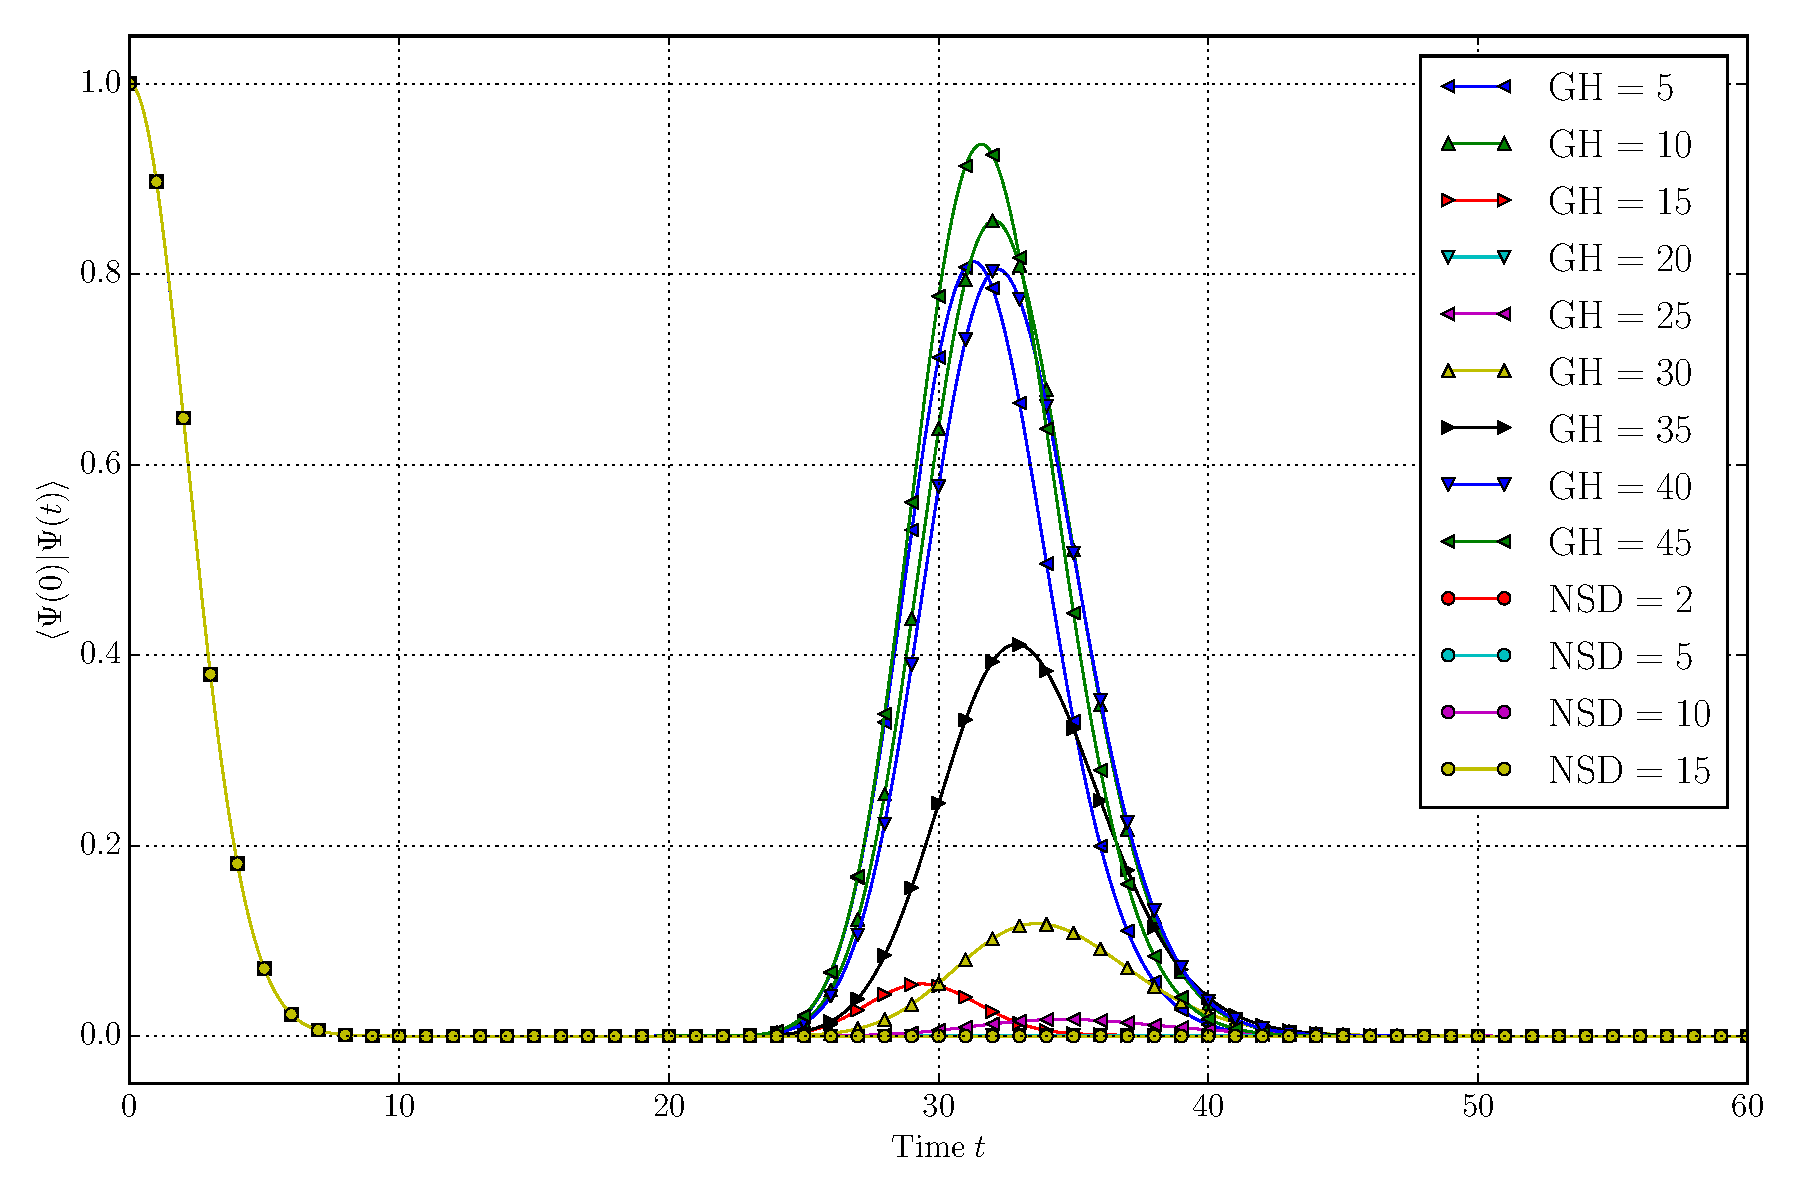
\includegraphics[width=\linewidth]{./fig/ac_mercurial_morse.pdf}
  \caption{Autocorrelation of the Mercury dynamics computed with classical
  Gauss-Hermite quadrature and with the steepest descent method each with several
  numbers of quadrature points. Only the numerical steepest descent transformation
  yields accurate results.}
  \label{fig:ac_mercurial_morse}
\end{figure}

Gauss-Hermite quadrature with any number of nodes shows high spurious autocorrelation bumps.
Using the steepest descent transformation before applying a quadrature scheme gives
correct results for an even smaller number of nodes.

In the following we will perform numerical simulations and shows the
robustness of this new technique.


\subsection{Two-Packet Experiment}

In this section we show the insufficiency of the Gauss-Hermite quadrature
for computing the integral in \eqref{eq:compute_ac_wavepackets}. The setup
of this experiment consists of two wavepackets $\phi[\Pi]$ and $\phi[\Pi^\prime]$.
Both are fixed in space at positions $q$ and $q^\prime$. Next we direct the
momenta $p$ and $p^\prime$ towards each other ($p^\prime = -p$) and start
increasing their magnitude $|p|$. The procedure is shown also in figure \ref{fig:convergence_setup}.

\begin{figure}[h!]
  \centering
  \includegraphics[width=0.5\linewidth]{./fig/convergence_setup.pdf}
  \caption{Setup of the first experiment. There are two wavepackets $\Psi$
    and $\Psi^\prime$ located next to each other at fixed positions $q$ and
    $q^\prime$. We set increasing momenta $p$ and $p^\prime$
    in opposite direction.}
  \label{fig:convergence_setup}
\end{figure}

The higher the momenta, the more oscillations appear in the product $\conj{\phi}(x) \phi^\prime(x)$.
These oscillations are difficult for Gauss Hermite quadrature to catch and it will
break down even for relatively small momenta. On the other hand, since the
steepest descent transformation applies to arbitrary high oscillator frequency,
it perfectly handles arbitrary momenta and converges fast to the correct
overlap integral value.

For the one-dimensional case there exists an analytic formula for computing
the integral. Evaluation is very expensive but can still server as exact
reference solution.


\FloatBarrier
\subsubsection{Convergence in $|p|$}


\begin{figure}
  \begin{subfigure}{0.5\linewidth}
    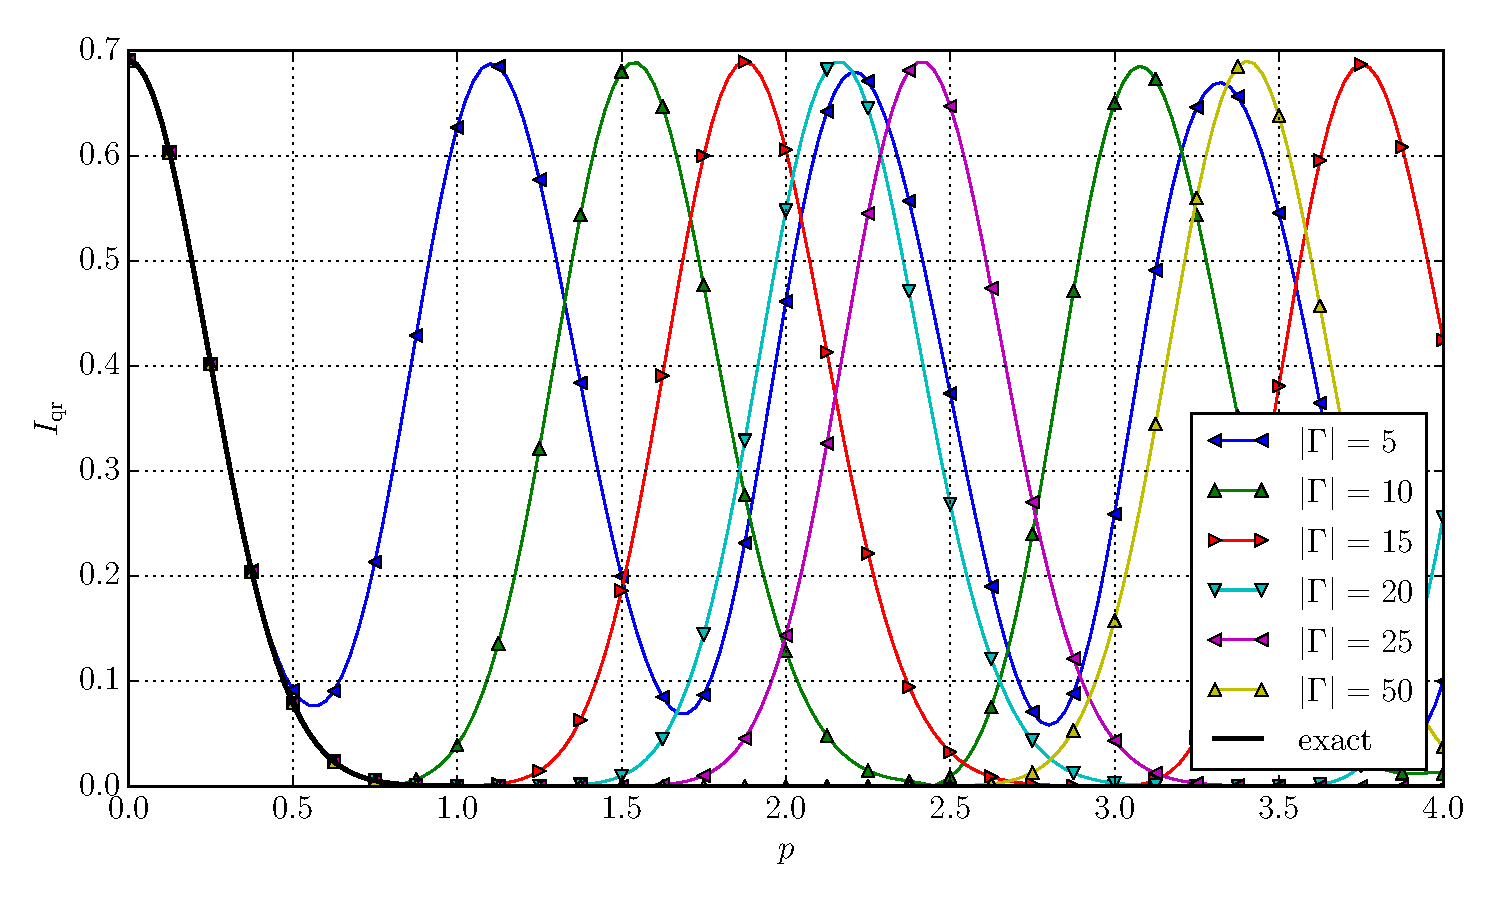
\includegraphics[width=\linewidth]{./plots/tp_1d_conv_p_0_0_val_qr.pdf}
    \caption{Gauss-Hermite quadrature with $|\Gamma|$ nodes.}
    \label{fig:tp_1d_conv_p_0_0_val_qr}
  \end{subfigure}
  \begin{subfigure}{0.5\linewidth}
    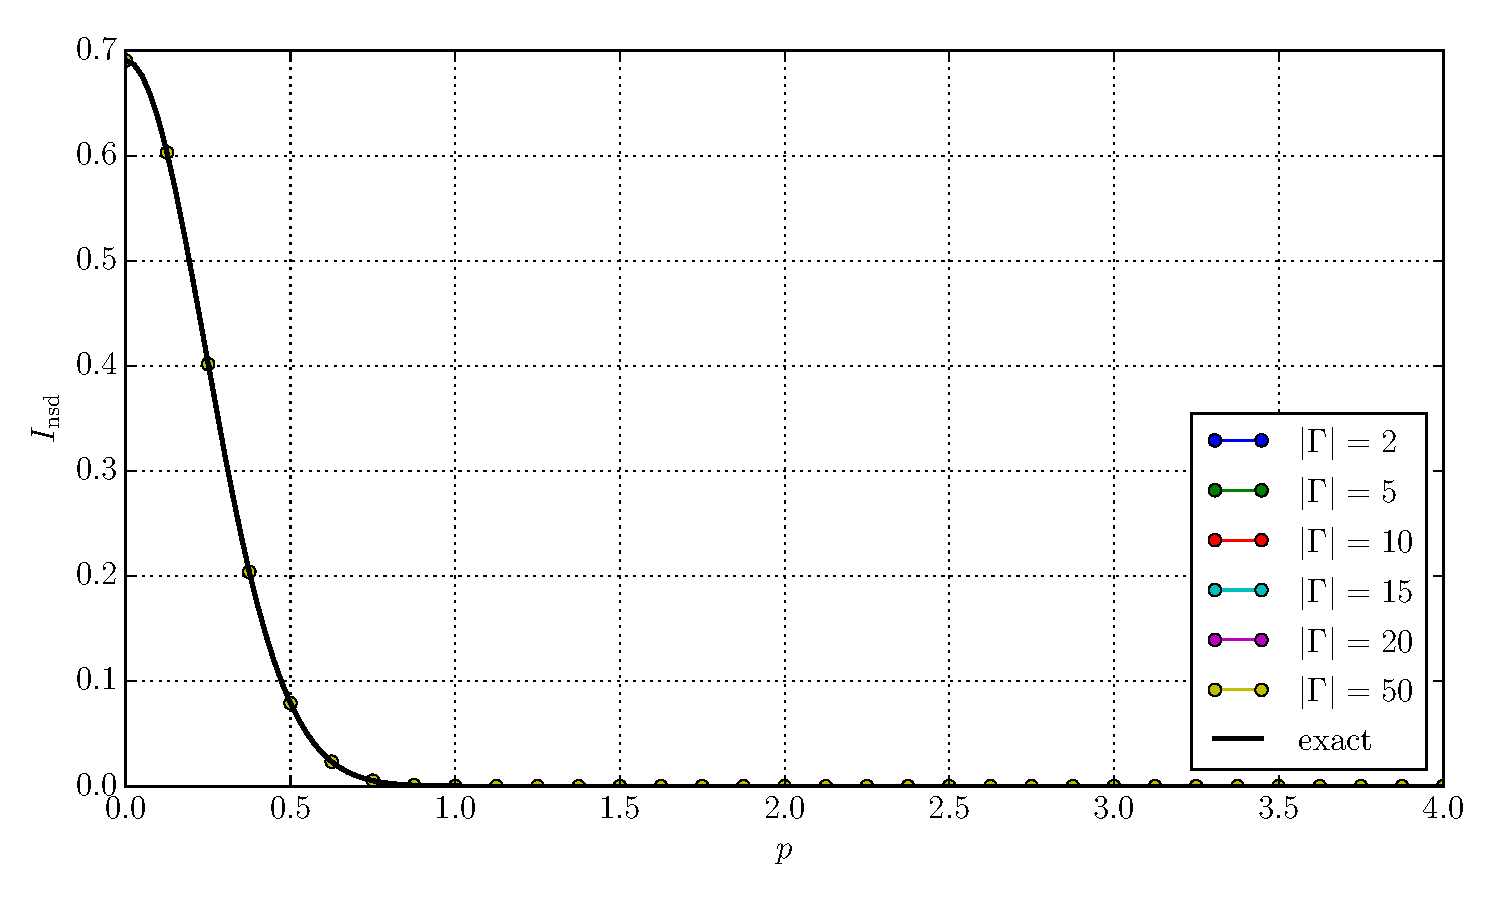
\includegraphics[width=\linewidth]{./plots/tp_1d_conv_p_0_0_val_nsd.pdf}
    \caption{Steepest descent transformation and quadrature with $|\Gamma|$ nodes.}
    \label{fig:tp_1d_conv_p_0_0_val_nsd}
  \end{subfigure} \\
  \begin{subfigure}{0.5\linewidth}
    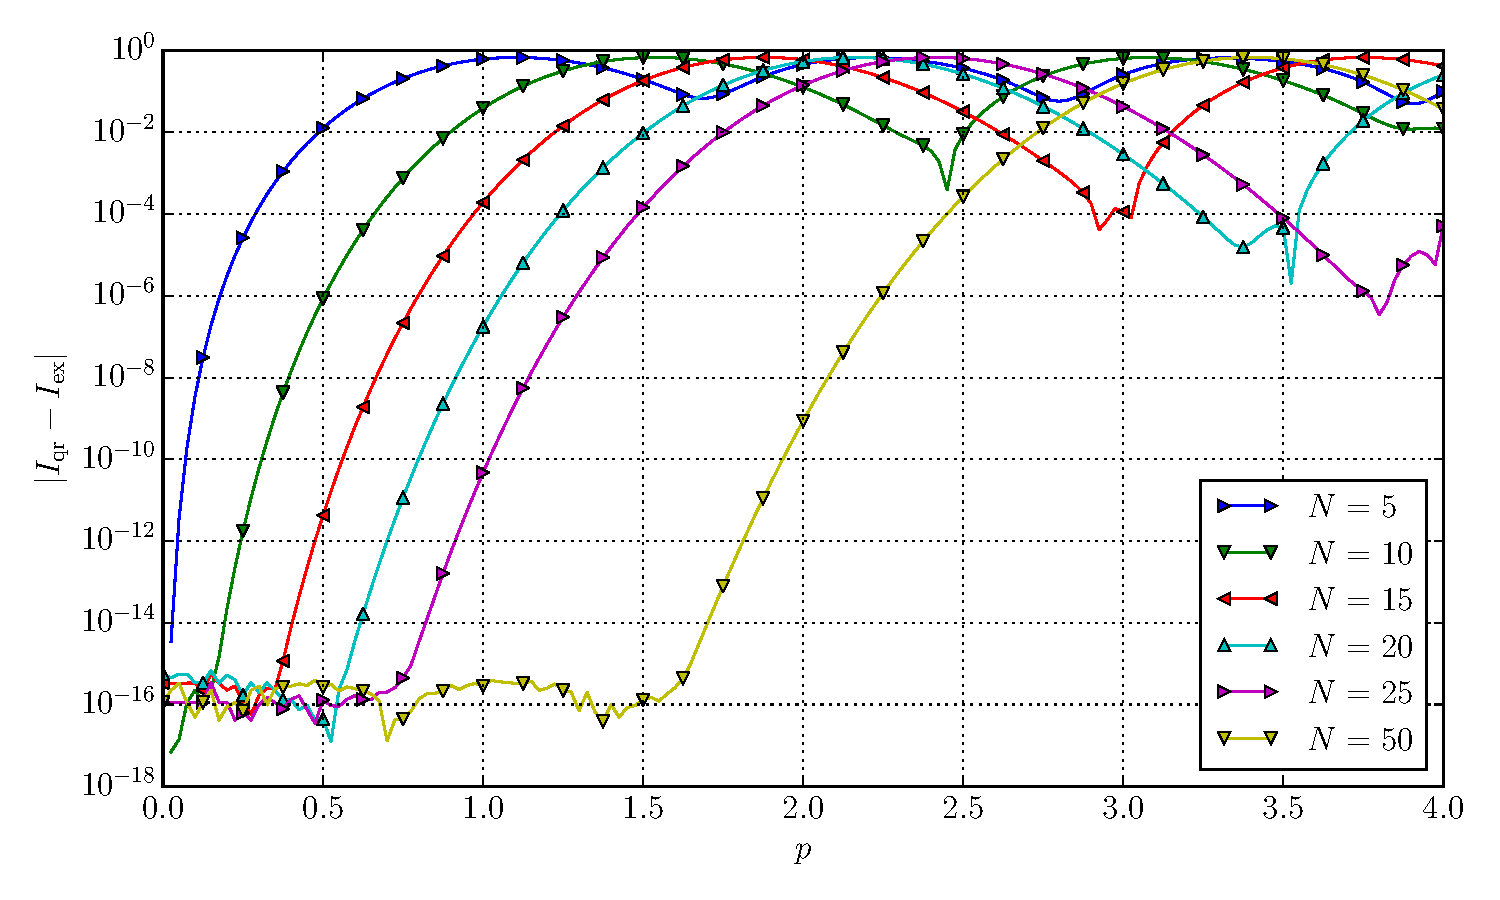
\includegraphics[width=\linewidth]{./plots/tp_1d_conv_p_0_0_err_qr.pdf}
    \caption{Absolute error of the Gauss-Hermite quadrature compared to the exact solution.}
    \label{fig:tp_1d_conv_p_0_0_err_qr}
  \end{subfigure}
  \begin{subfigure}{0.5\linewidth}
    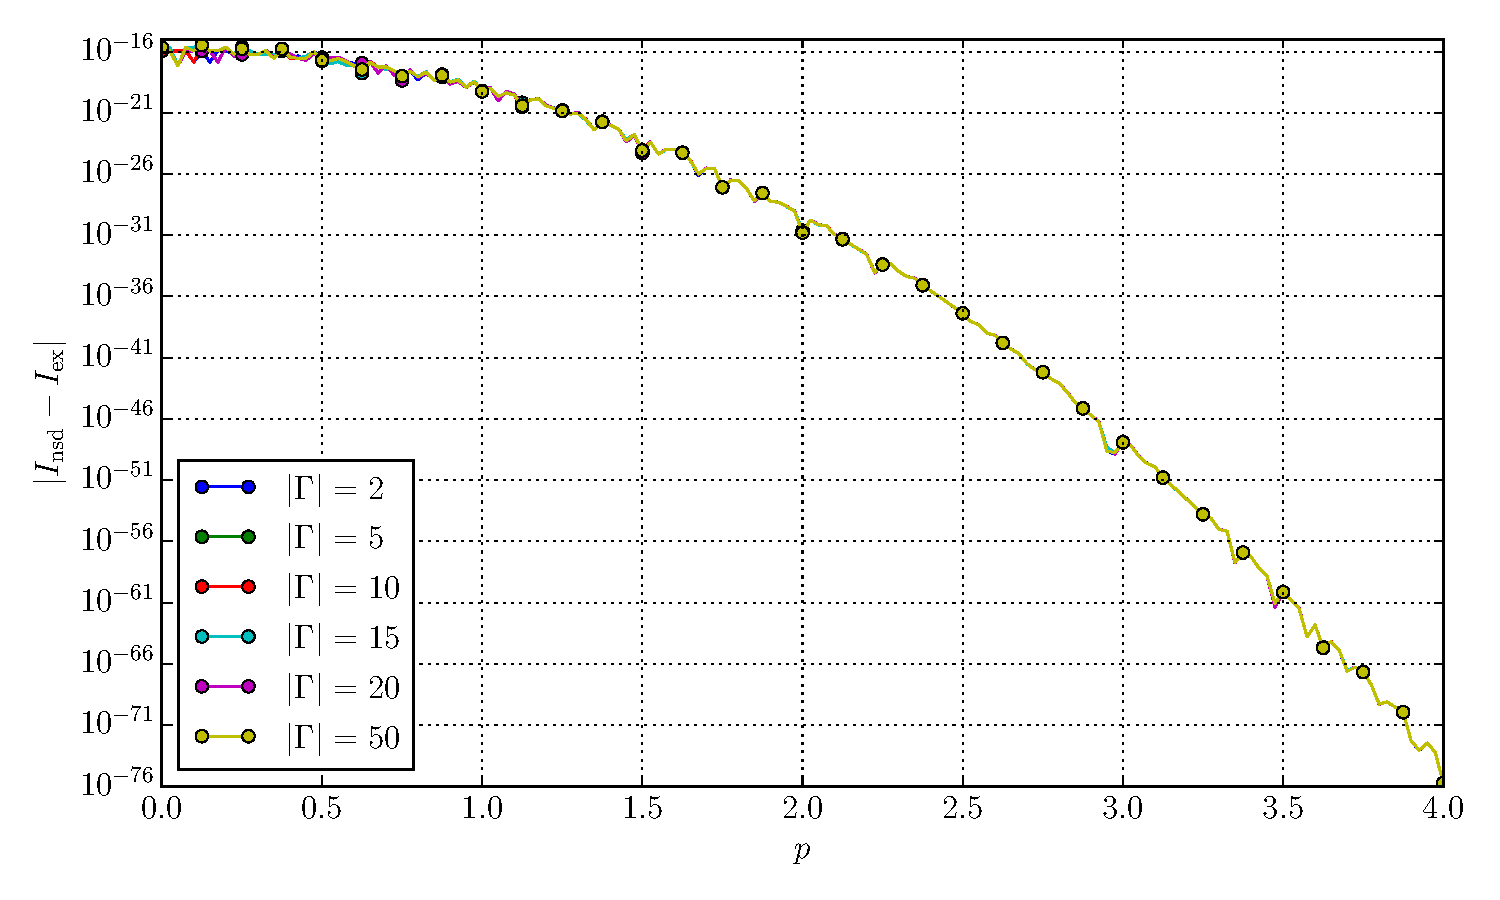
\includegraphics[width=\linewidth]{./plots/tp_1d_conv_p_0_0_err_nsd.pdf}
    \caption{Absolute error of the steepest descent method compared to the exact solution.}
    \label{fig:tp_1d_conv_p_0_0_err_nsd}
  \end{subfigure}
  \begin{subfigure}{0.5\linewidth}
    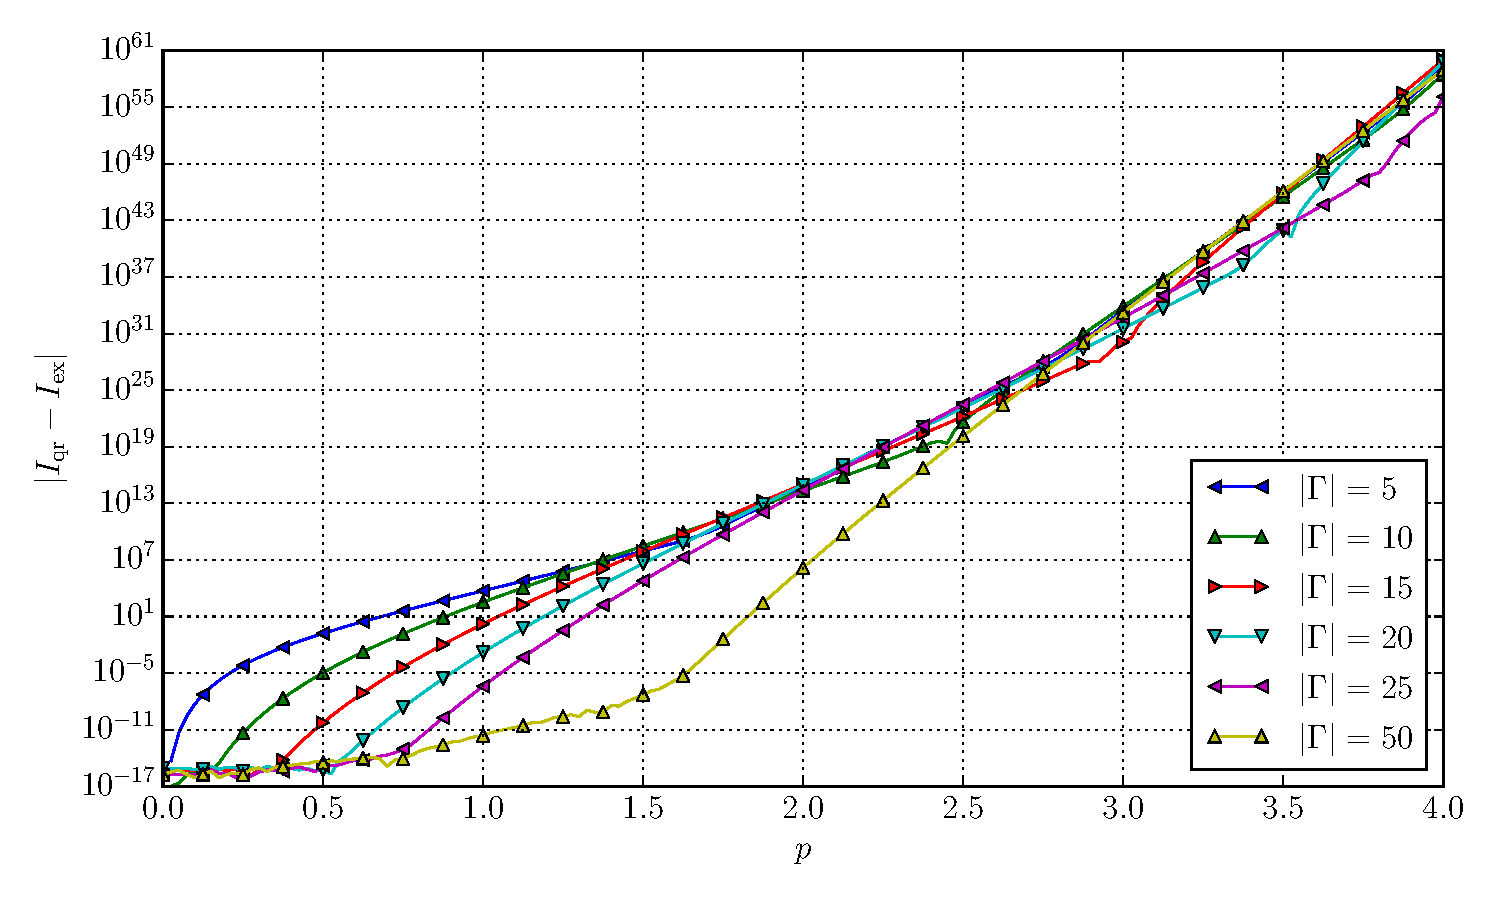
\includegraphics[width=\linewidth]{./plots/tp_1d_conv_p_0_0_err_rel_qr.pdf}
    \caption{Relative error of the Gauss-Hermite quadrature compared to the exact solution.}
    \label{fig:tp_1d_conv_p_0_0_err_qr}
  \end{subfigure}
  \begin{subfigure}{0.5\linewidth}
    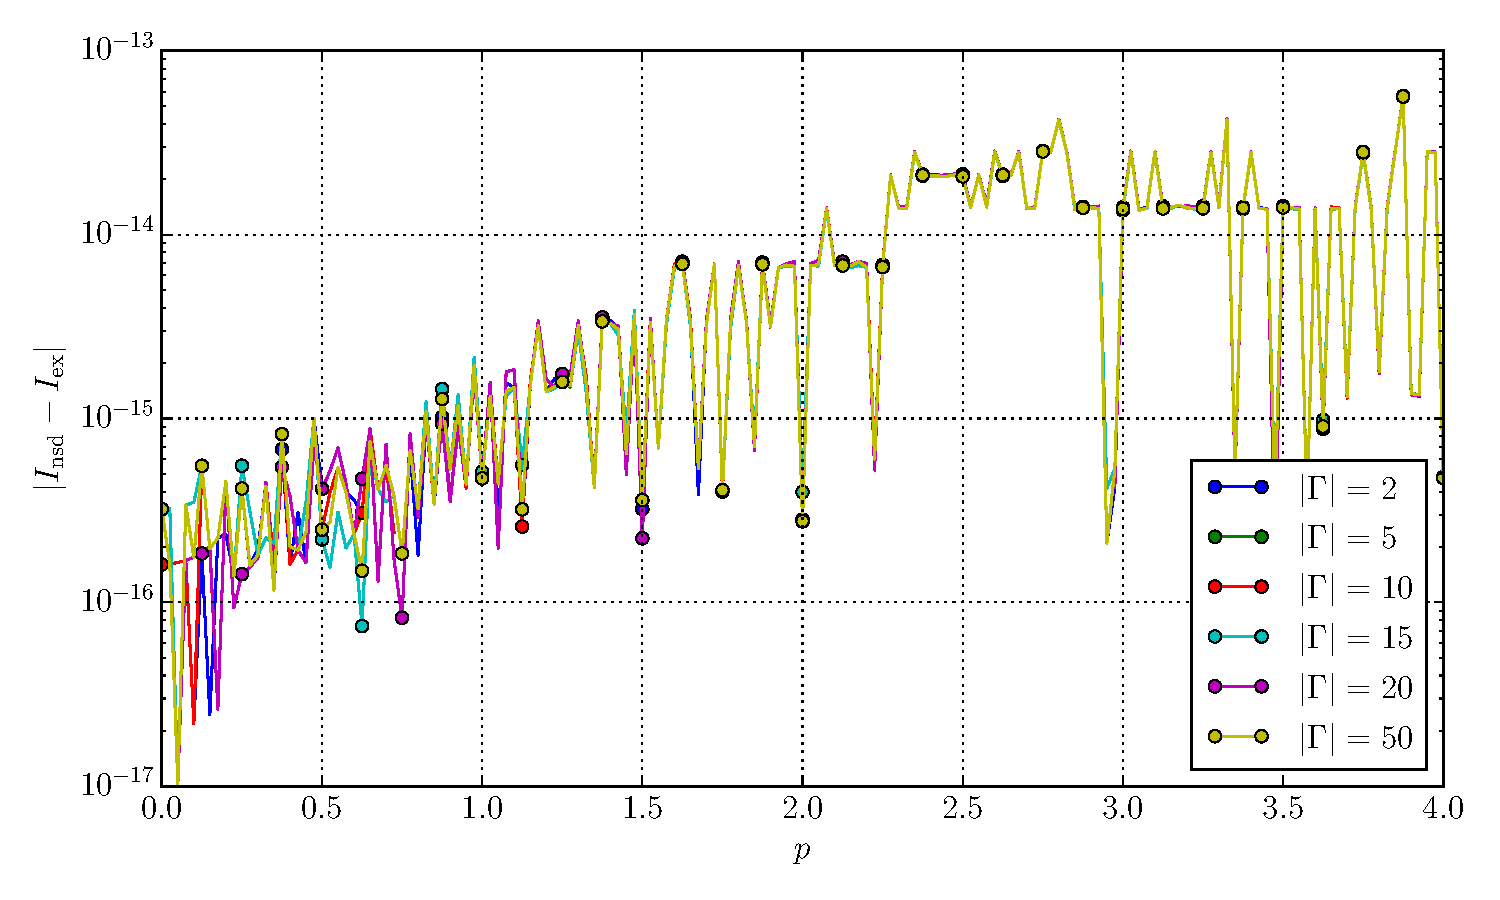
\includegraphics[width=\linewidth]{./plots/tp_1d_conv_p_0_0_err_rel_nsd.pdf}
    \caption{Relative error of the steepest descent method compared to the exact solution.}
    \label{fig:tp_1d_conv_p_0_0_err_nsd}
  \end{subfigure}
  \label{fig:tp_1d_conv_p_0_0}
  \caption{Experiment with $\phi_{0}$ and $\phi_{0}^{\prime}$.
  The parameters are:
  $q=-0.2$, $p=1.5$, $Q=1.0$, $P=1.0\imath$ and
  $q^\prime=0.125$, $p^\prime=-1.5$, $Q^\prime=0.8$, $P^\prime=1.25\imath$
  with $\varepsilon = 0.3$.}
\end{figure}

\begin{figure}
  \begin{subfigure}{0.5\linewidth}
    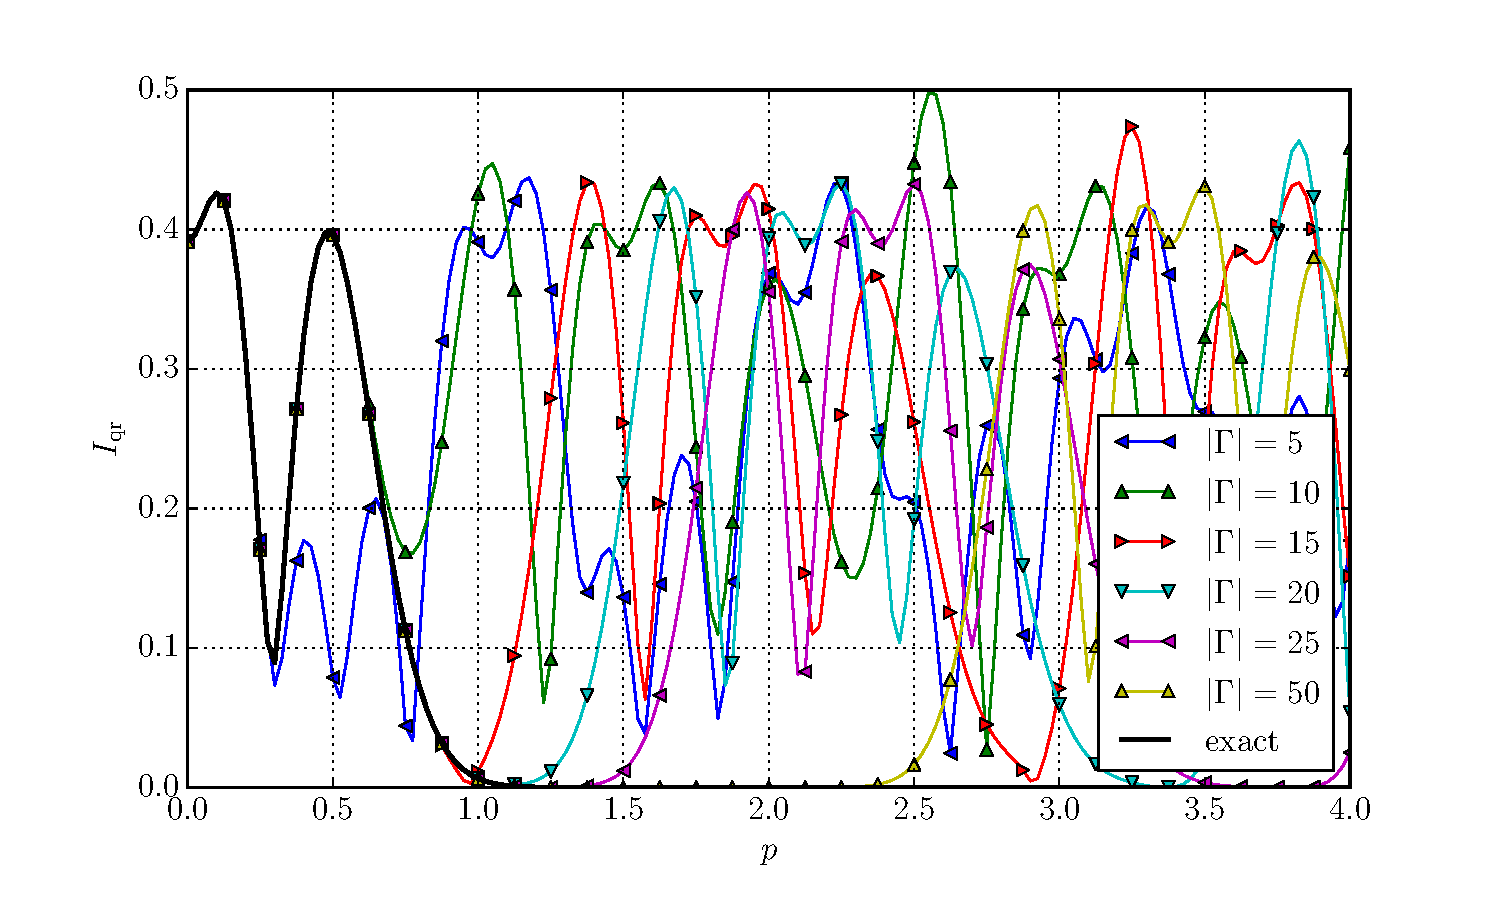
\includegraphics[width=\linewidth]{./plots/tp_1d_conv_p_2_1_val_qr.pdf}
    \caption{Gauss-Hermite quadrature with $|\Gamma|$ nodes.}
    \label{fig:tp_1d_conv_p_2_1_val_qr}
  \end{subfigure}
  \begin{subfigure}{0.5\linewidth}
    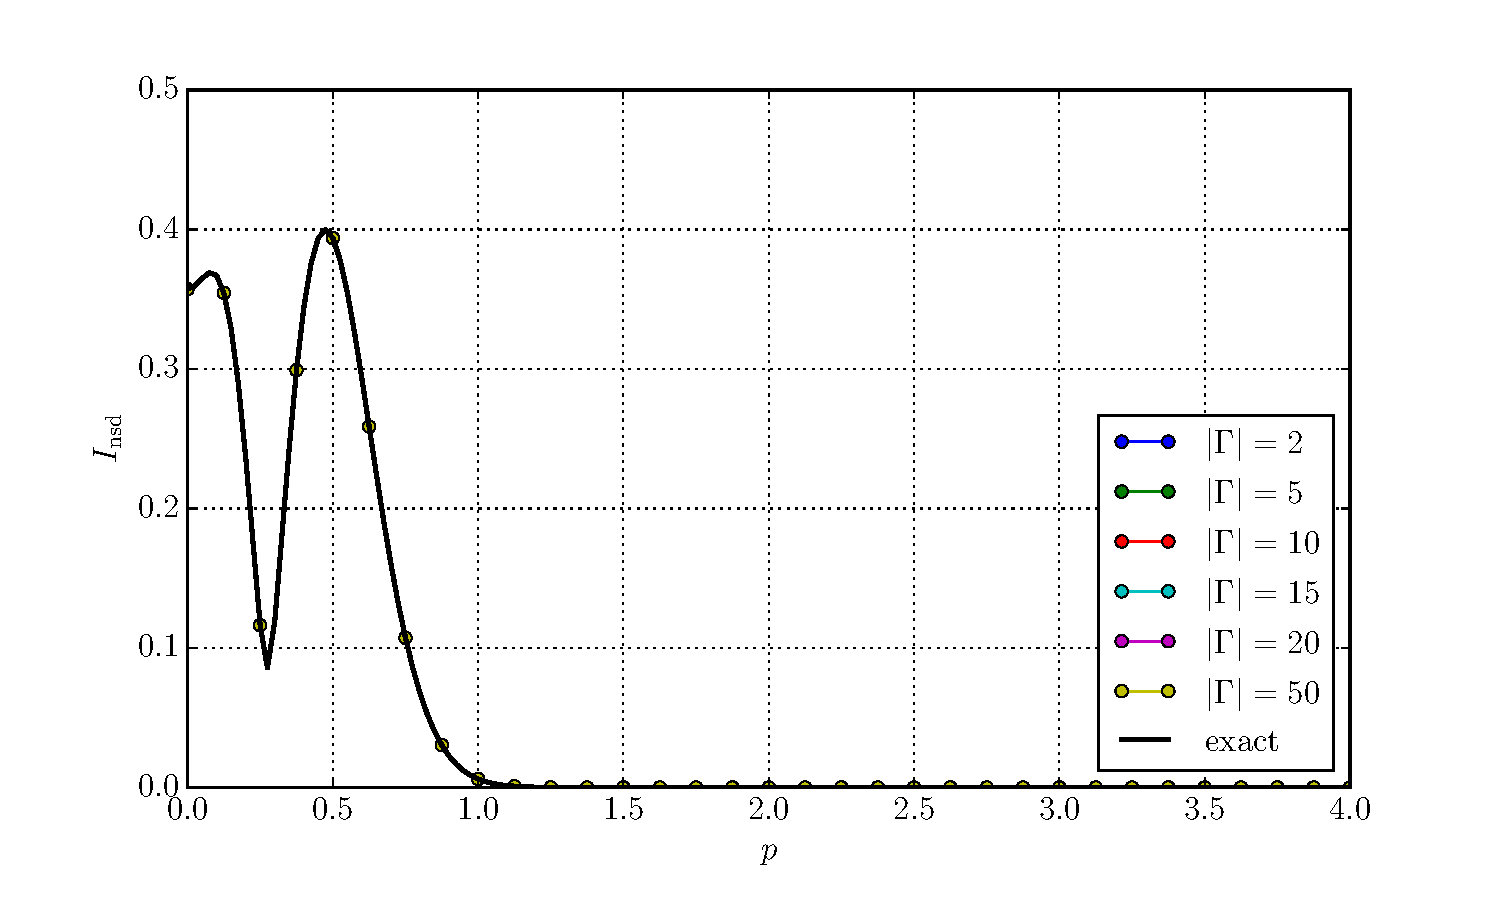
\includegraphics[width=\linewidth]{./plots/tp_1d_conv_p_2_1_val_nsd.pdf}
    \caption{Steepest descent transformation and quadrature with $|\Gamma|$ nodes.}
    \label{fig:tp_1d_conv_p_2_1_val_nsd}
  \end{subfigure} \\
  \begin{subfigure}{0.5\linewidth}
    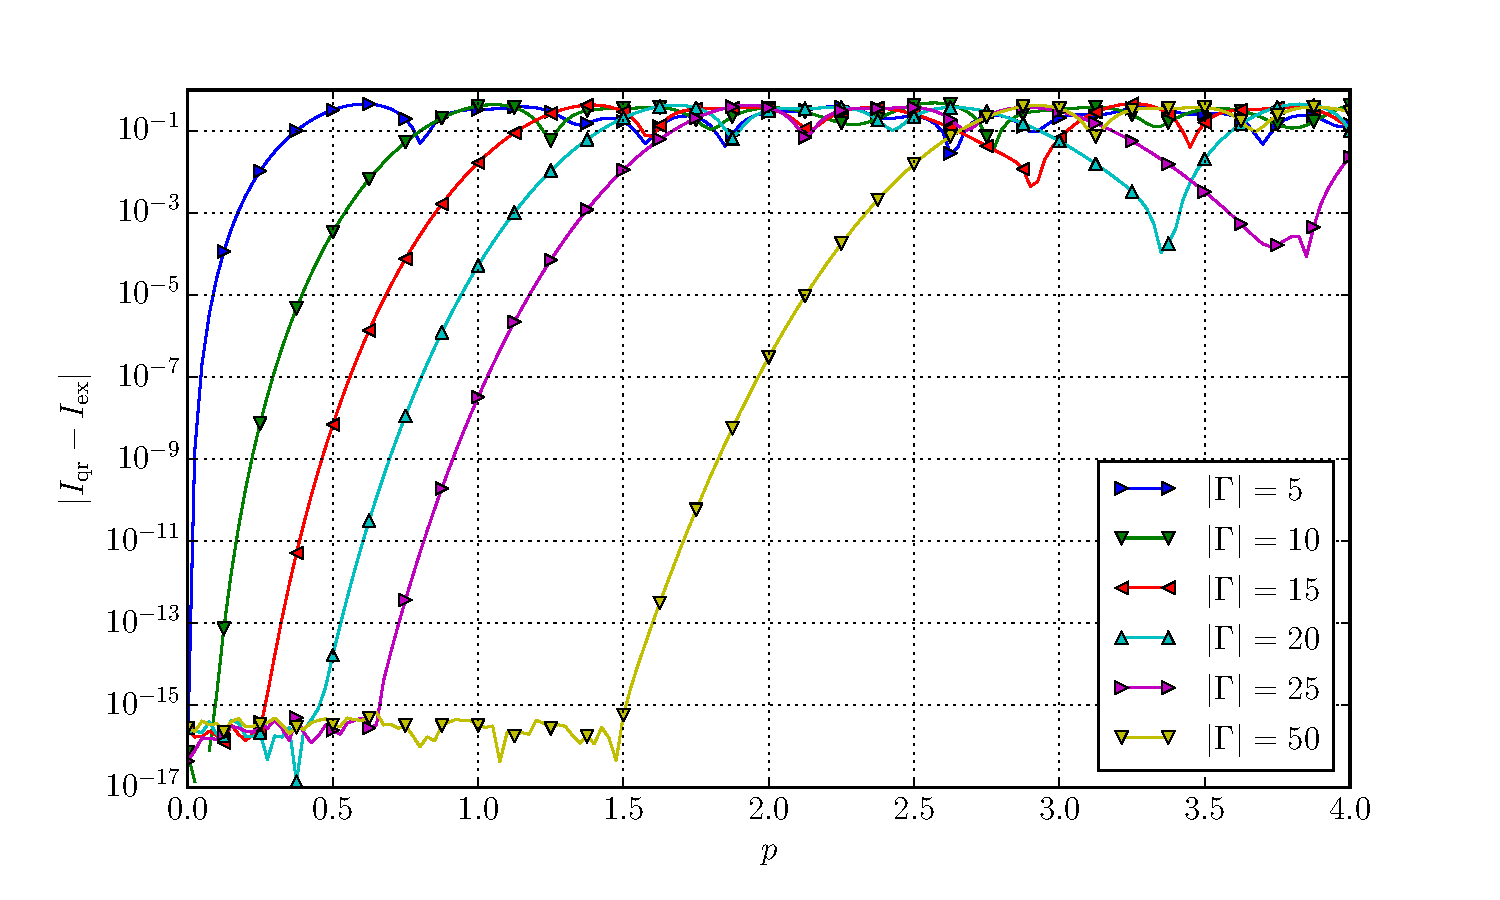
\includegraphics[width=\linewidth]{./plots/tp_1d_conv_p_2_1_err_qr.pdf}
    \caption{Absolute error of the Gauss-Hermite quadrature compared to the exact solution.}
    \label{fig:tp_1d_conv_p_2_1_err_qr}
  \end{subfigure}
  \begin{subfigure}{0.5\linewidth}
    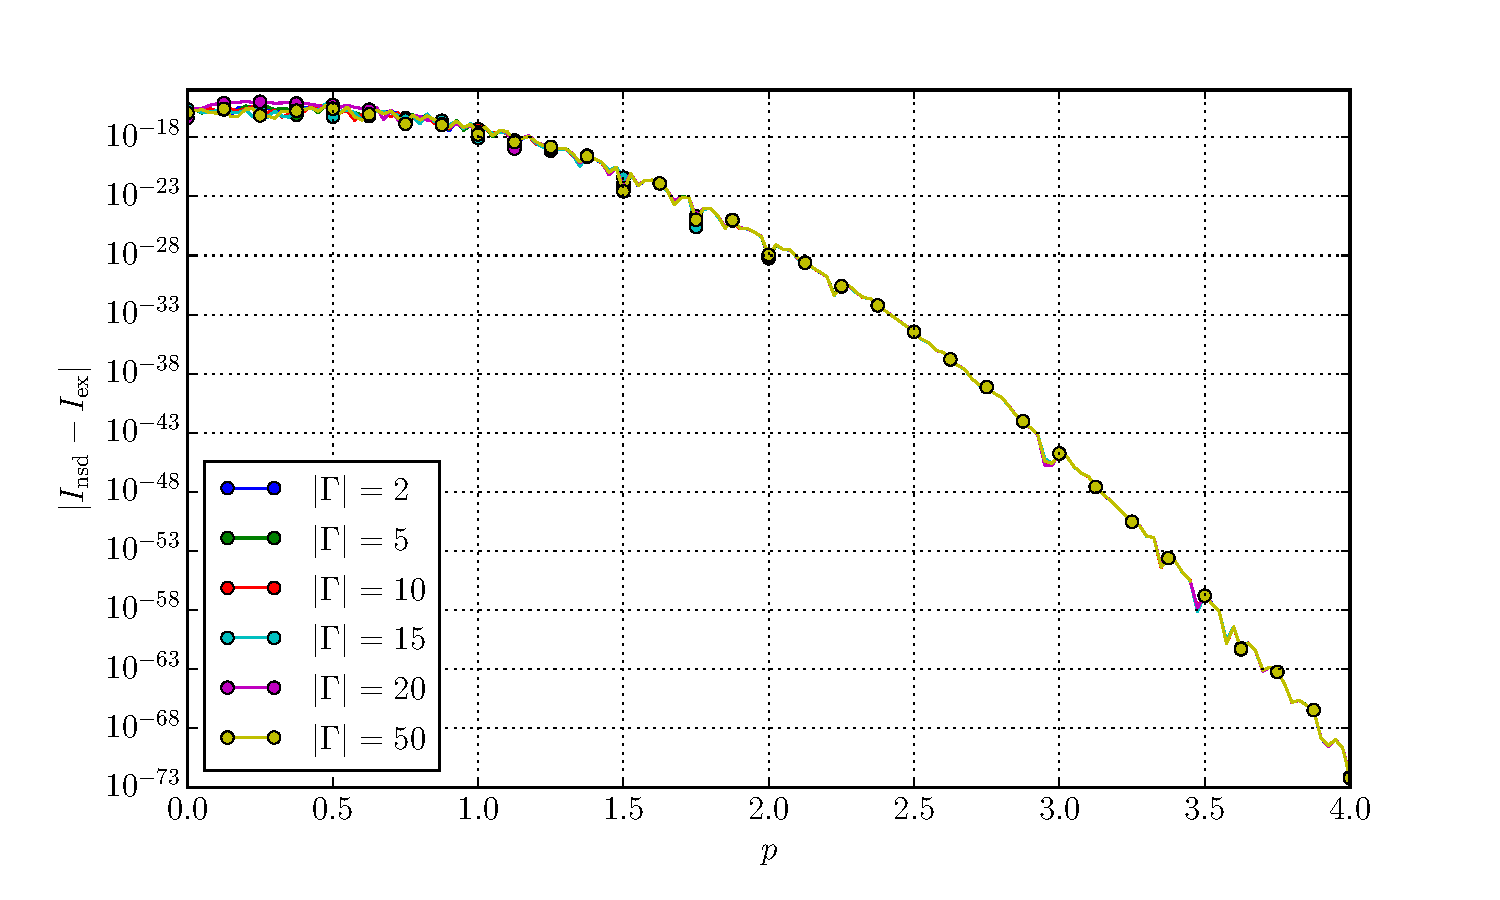
\includegraphics[width=\linewidth]{./plots/tp_1d_conv_p_2_1_err_nsd.pdf}
    \caption{Absolute error of the steepest descent method compared to the exact solution.}
    \label{fig:tp_1d_conv_p_2_1_err_nsd}
  \end{subfigure}
  \begin{subfigure}{0.5\linewidth}
    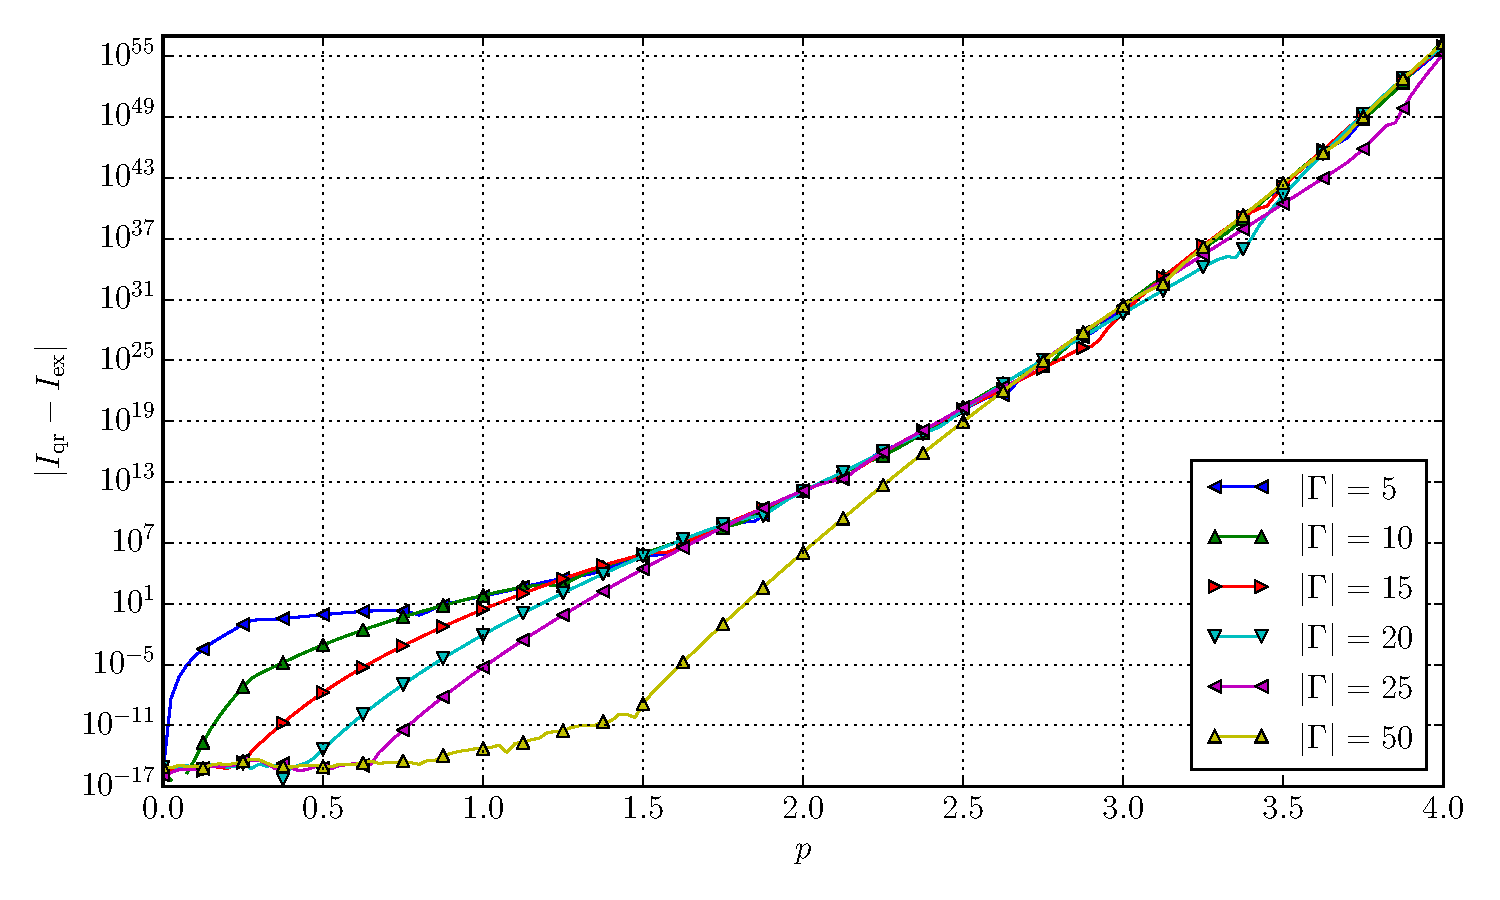
\includegraphics[width=\linewidth]{./plots/tp_1d_conv_p_2_1_err_rel_qr.pdf}
    \caption{Relative error of the Gauss-Hermite quadrature compared to the exact solution.}
    \label{fig:tp_1d_conv_p_2_1_err_qr}
  \end{subfigure}
  \begin{subfigure}{0.5\linewidth}
    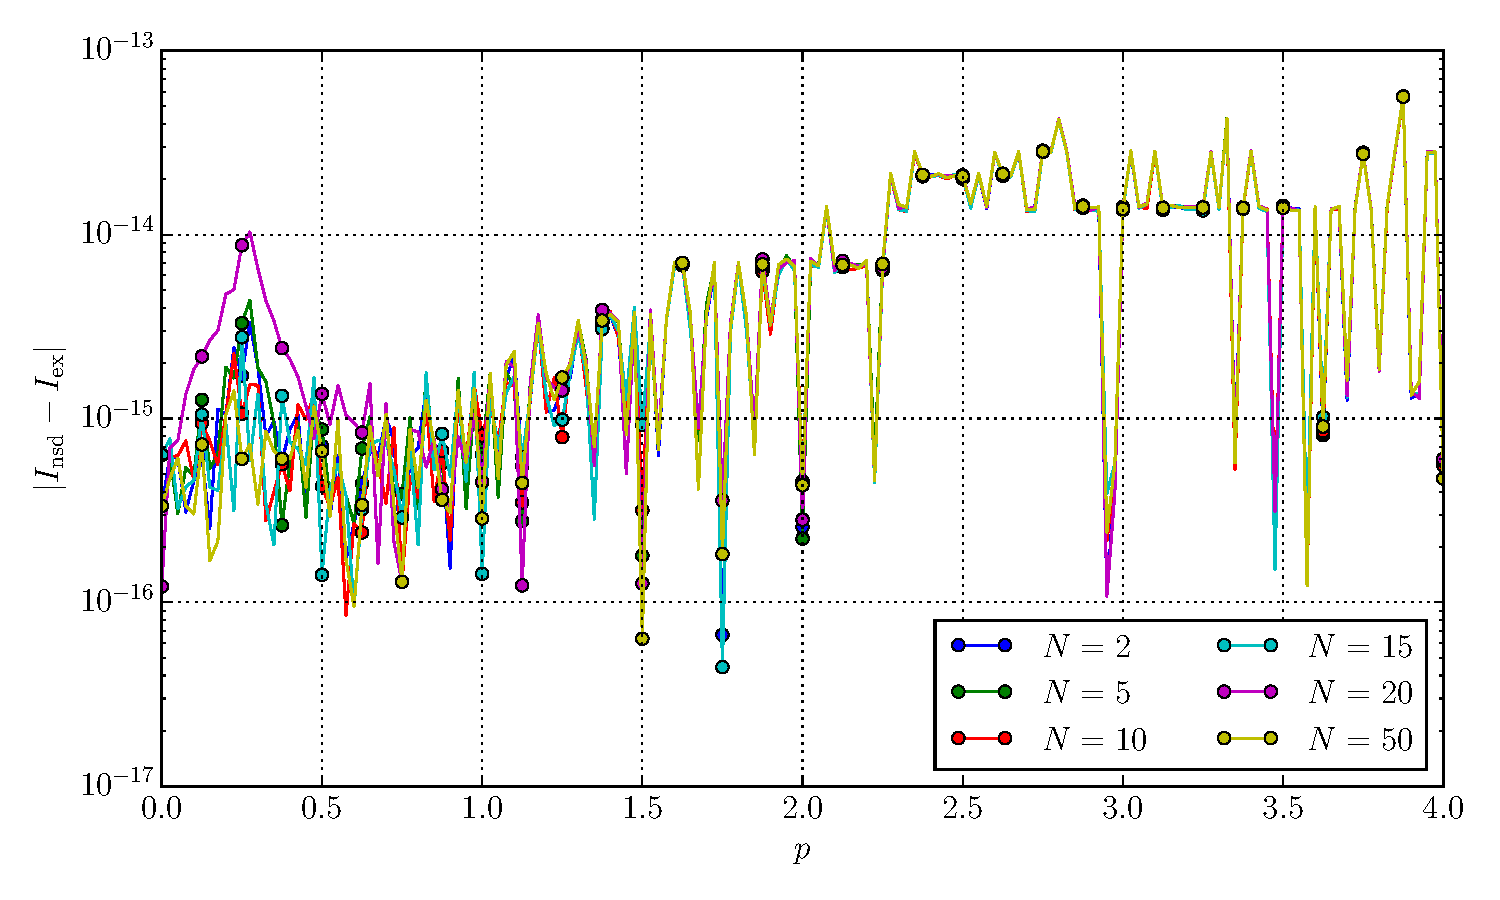
\includegraphics[width=\linewidth]{./plots/tp_1d_conv_p_2_1_err_rel_nsd.pdf}
    \caption{Relative error of the steepest descent method compared to the exact solution.}
    \label{fig:tp_1d_conv_p_2_1_err_nsd}
  \end{subfigure}
  \label{fig:tp_1d_conv_p_2_1}
  \caption{Experiment with $\phi_{2}$ and $\phi_{1}^{\prime}$.
  The parameters are:
  $q=-0.2$, $p=1.5$, $Q=1.0$, $P=1.0\imath$ and
  $q^\prime=0.125$, $p^\prime=-1.5$, $Q^\prime=0.8$, $P^\prime=1.25\imath$
  with $\varepsilon = 0.3$.}
\end{figure}

\begin{figure}
  \begin{subfigure}{0.5\linewidth}
    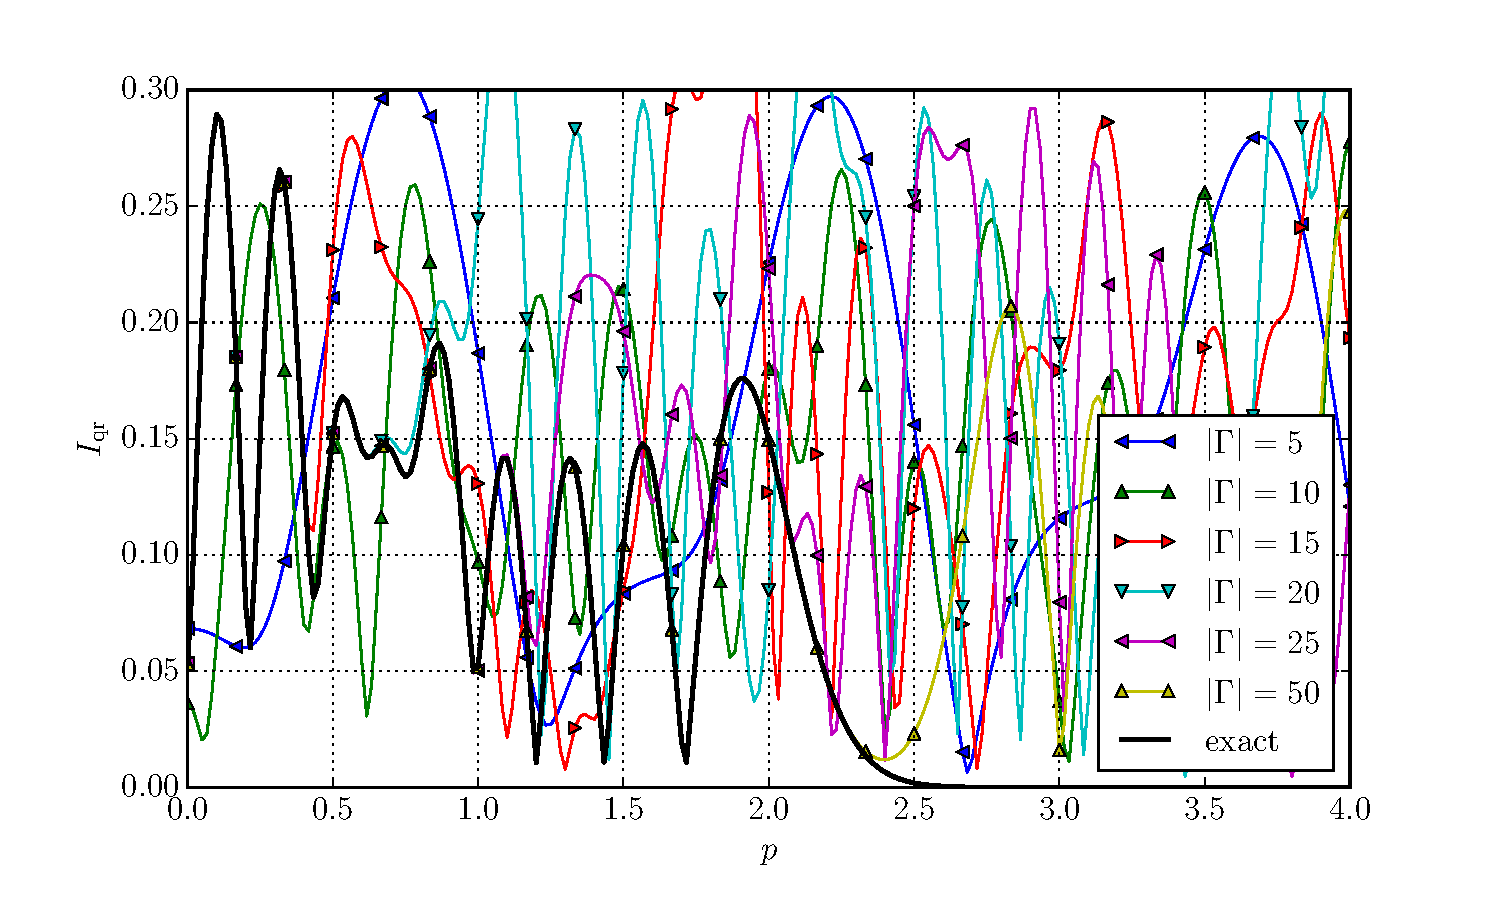
\includegraphics[width=\linewidth]{./plots/tp_1d_conv_p_11_9_val_qr.pdf}
    \caption{Gauss-Hermite quadrature with $|\Gamma|$ nodes.}
    \label{fig:tp_1d_conv_p_11_9_val_qr}
  \end{subfigure}
  \begin{subfigure}{0.5\linewidth}
    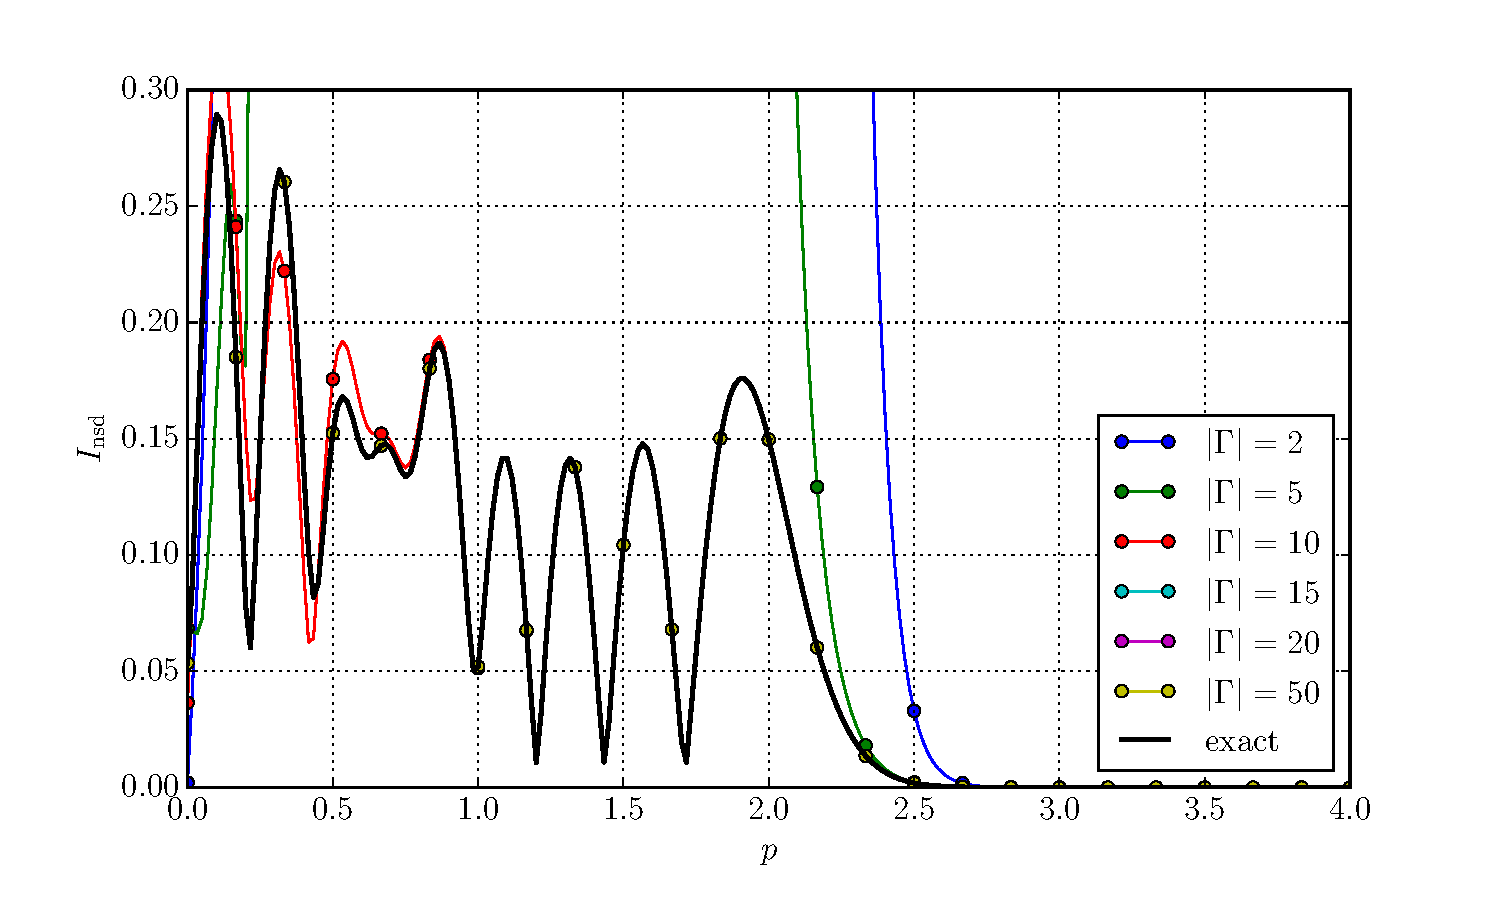
\includegraphics[width=\linewidth]{./plots/tp_1d_conv_p_11_9_val_nsd.pdf}
    \caption{Steepest descent transformation and quadrature with $|\Gamma|$ nodes.}
    \label{fig:tp_1d_conv_p_11_9_val_nsd}
  \end{subfigure} \\
  \begin{subfigure}{0.5\linewidth}
    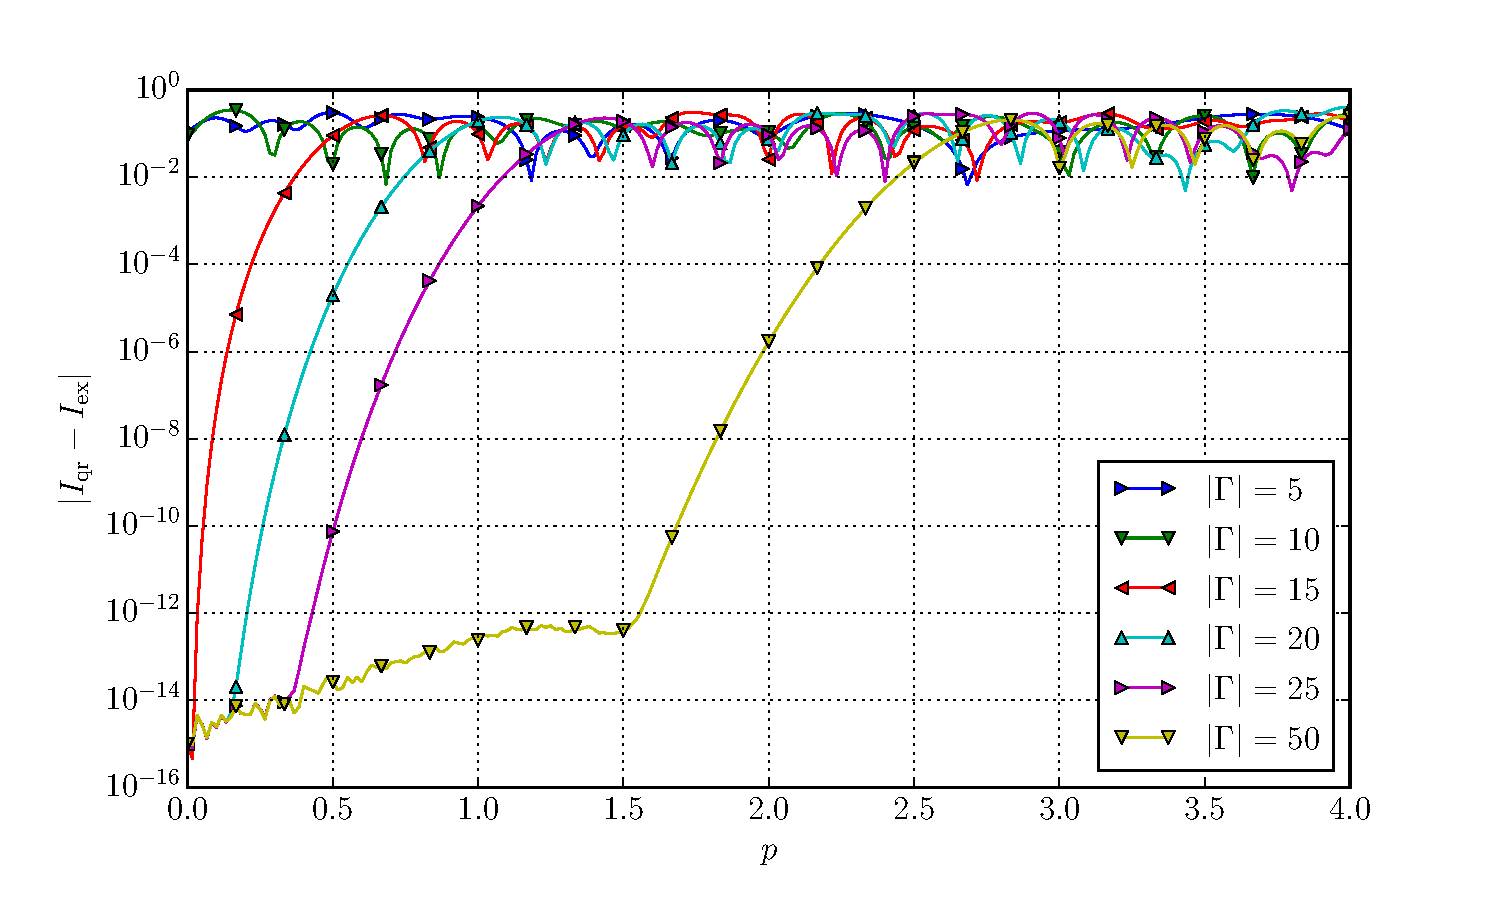
\includegraphics[width=\linewidth]{./plots/tp_1d_conv_p_11_9_err_qr.pdf}
    \caption{Absolute error of the Gauss-Hermite quadrature compared to the exact solution.}
    \label{fig:tp_1d_conv_p_11_9_err_qr}
  \end{subfigure}
  \begin{subfigure}{0.5\linewidth}
    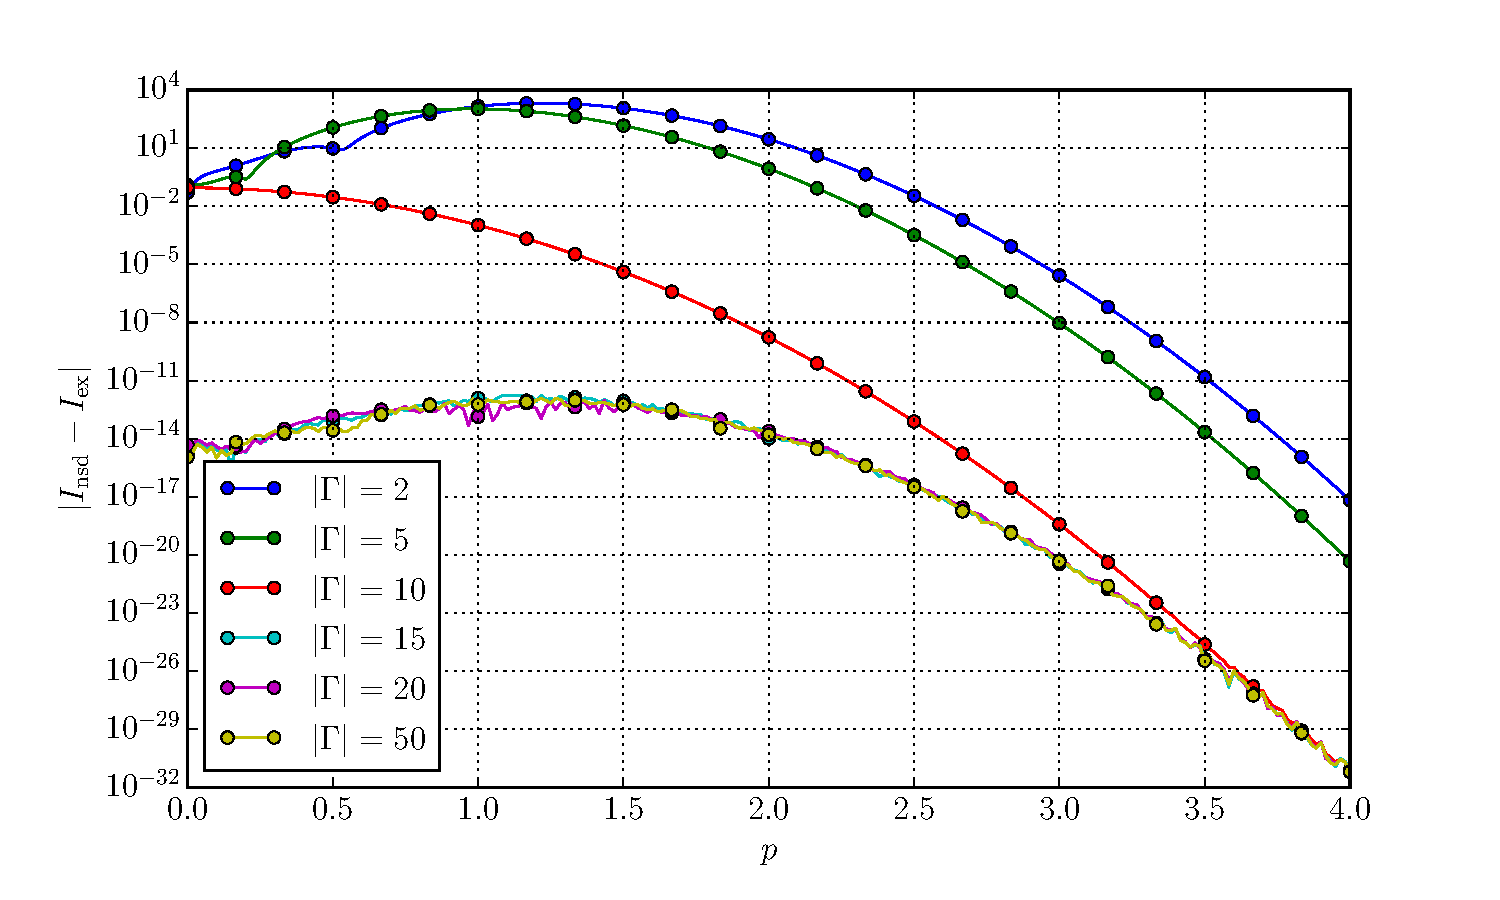
\includegraphics[width=\linewidth]{./plots/tp_1d_conv_p_11_9_err_nsd.pdf}
    \caption{Absolute error of the steepest descent method compared to the exact solution.}
    \label{fig:tp_1d_conv_p_11_9_err_nsd}
  \end{subfigure}
  \begin{subfigure}{0.5\linewidth}
    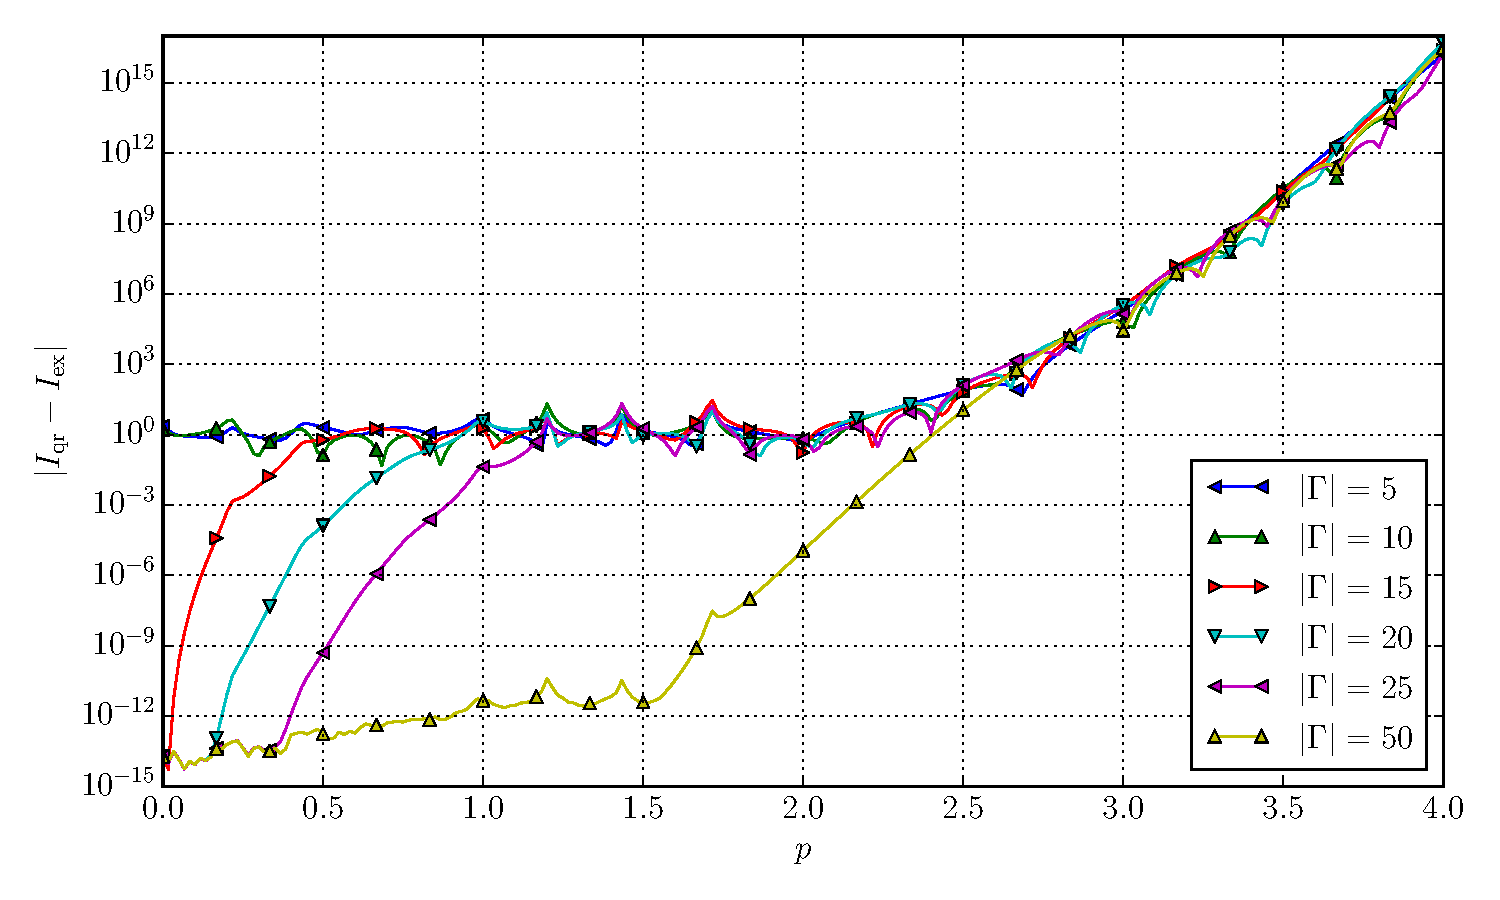
\includegraphics[width=\linewidth]{./plots/tp_1d_conv_p_11_9_err_rel_qr.pdf}
    \caption{Relative error of the Gauss-Hermite quadrature compared to the exact solution.}
    \label{fig:tp_1d_conv_p_11_9_err_qr}
  \end{subfigure}
  \begin{subfigure}{0.5\linewidth}
    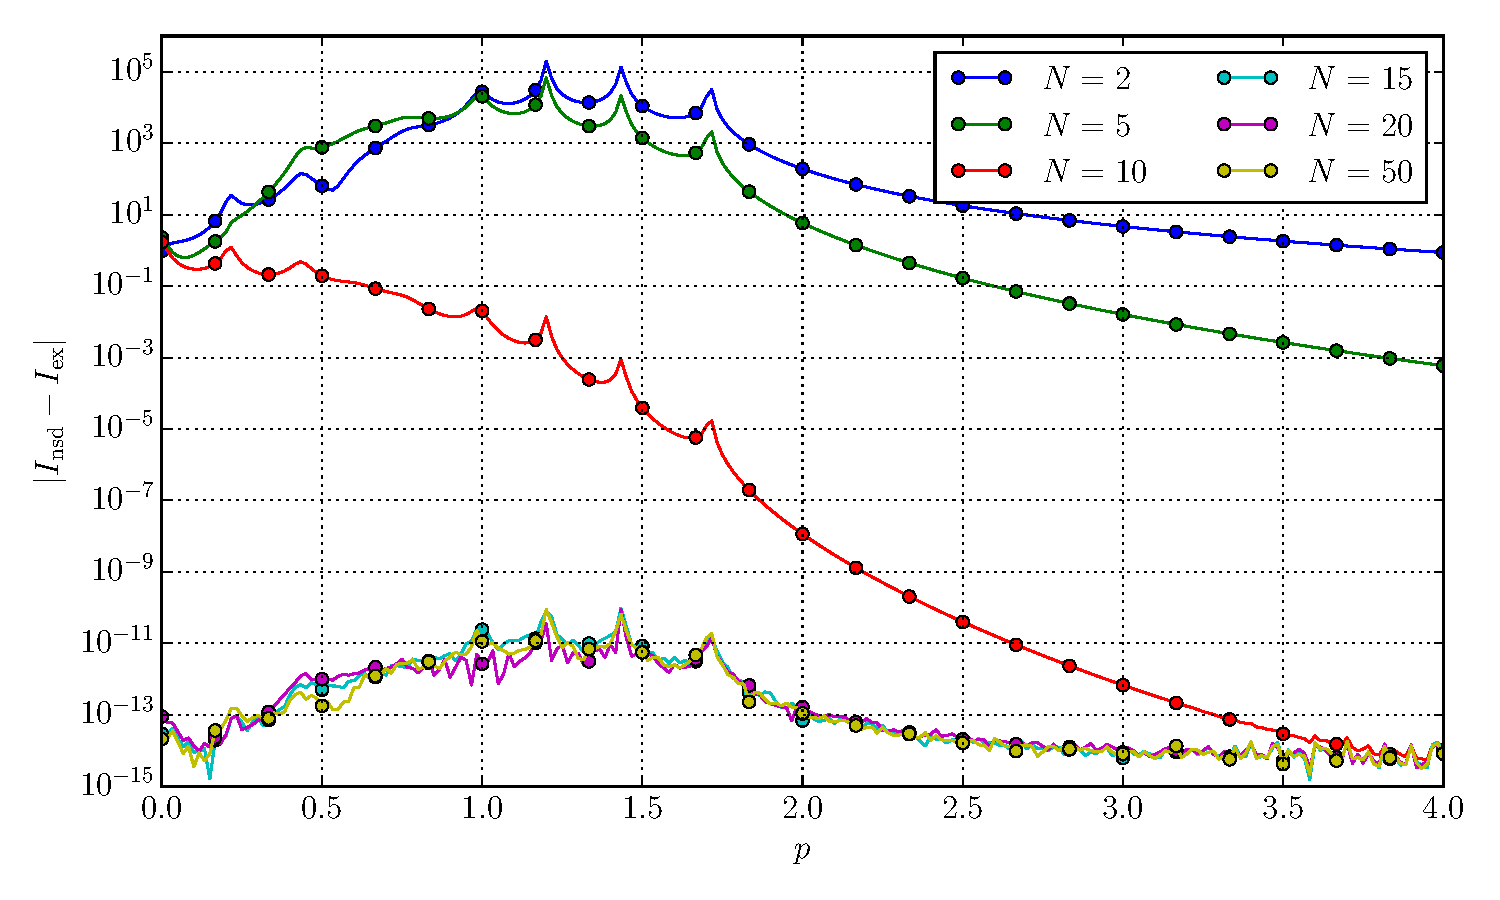
\includegraphics[width=\linewidth]{./plots/tp_1d_conv_p_11_9_err_rel_nsd.pdf}
    \caption{Relative error of the steepest descent method compared to the exact solution.}
    \label{fig:tp_1d_conv_p_11_9_err_nsd}
  \end{subfigure}
  \label{fig:tp_1d_conv_p_2_1}
  \caption{Experiment with $\phi_{11}$ and $\phi_{9}^{\prime}$.
  The parameters are:
  $q=-0.2$, $p=1.2$, $Q=1.0$, $P=1.0\imath$ and
  $q^\prime=0.2$, $p^\prime=-1.2$, $Q^\prime=0.5$, $P^\prime=2.0\imath$
  with $\varepsilon=0.3$.}
\end{figure}

\marginpar{comment figures}
\marginpar{oscillation in polynomial}

\begin{figure}
  \begin{subfigure}{0.5\linewidth}
    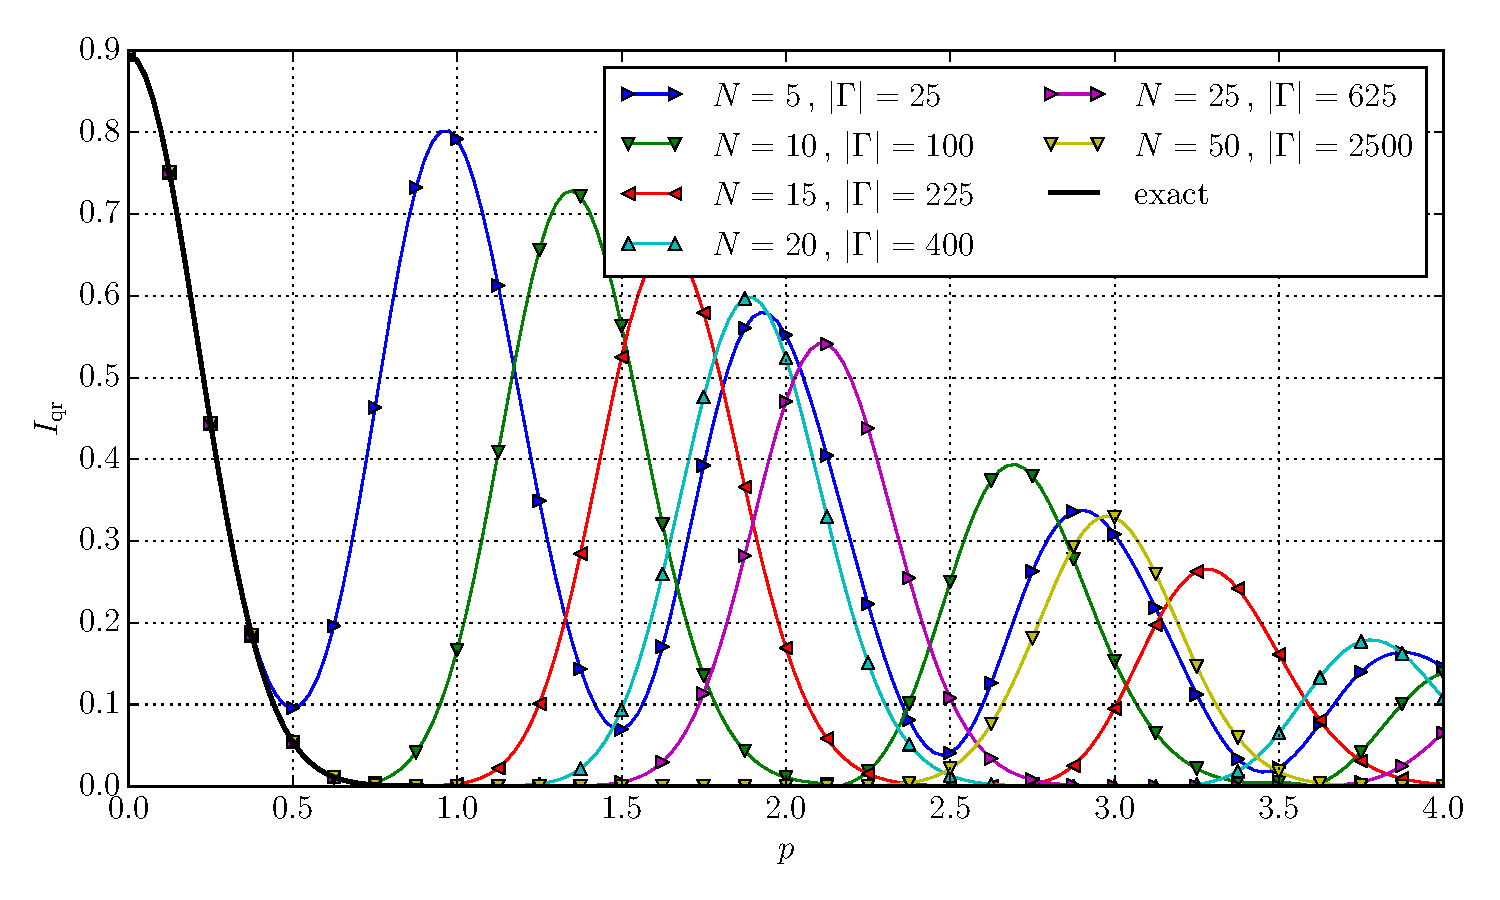
\includegraphics[width=\linewidth]{./plots/tp_2d_conv_p_(0,0)_(0,0)_val_qr.pdf}
    \caption{Gauss-Hermite quadrature with $|\Gamma|$ nodes.}
    \label{fig:tp_2d_conv_p_00_00_val_qr}
  \end{subfigure}
  \begin{subfigure}{0.5\linewidth}
    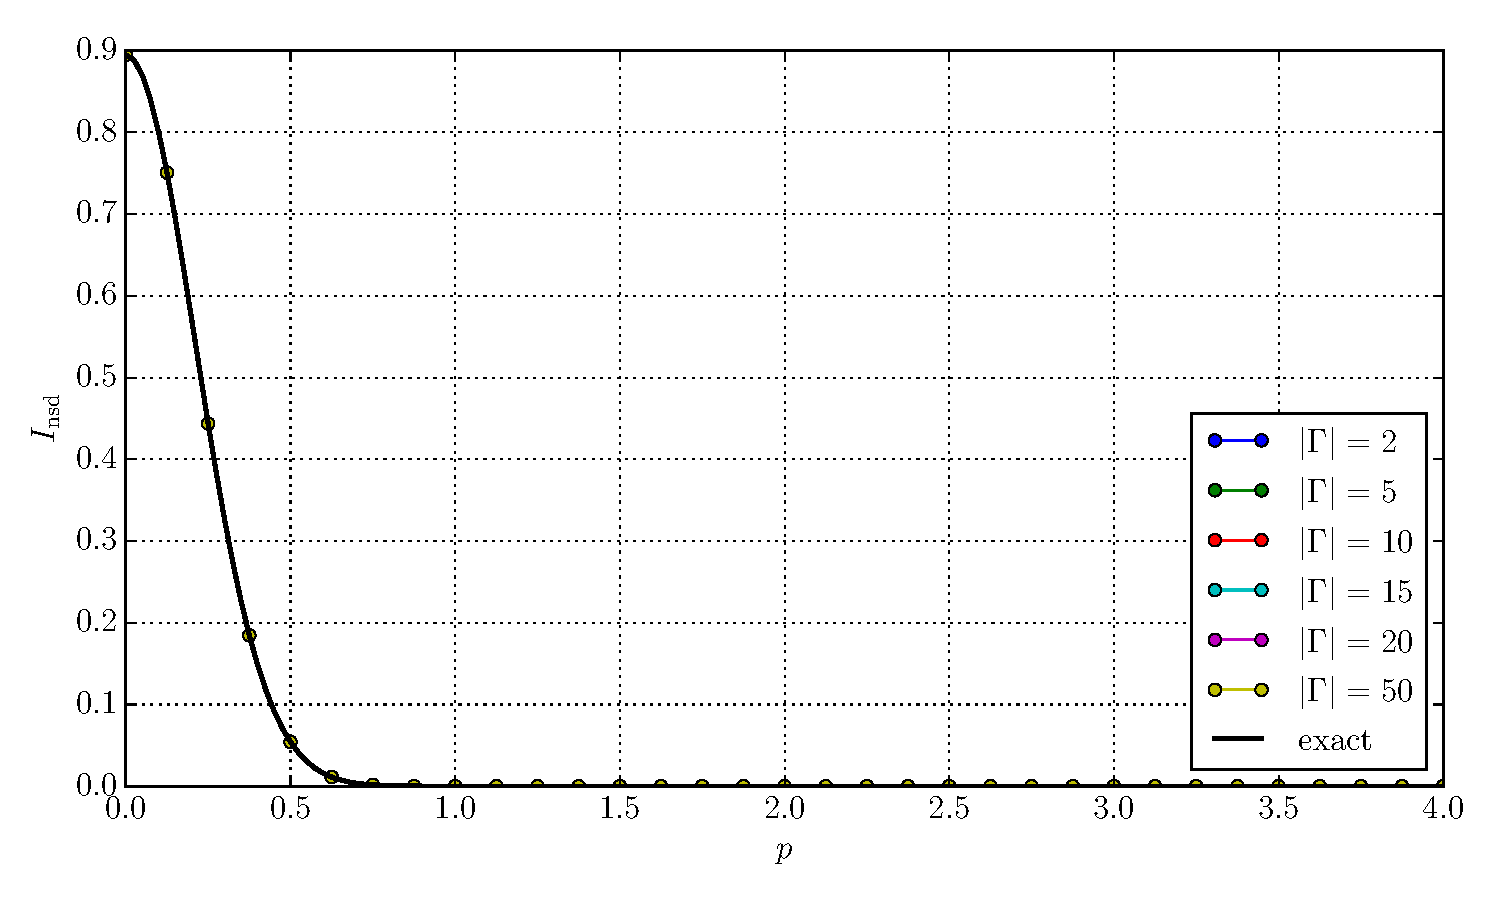
\includegraphics[width=\linewidth]{./plots/tp_2d_conv_p_(0,0)_(0,0)_val_nsd.pdf}
    \caption{Steepest descent transformation and quadrature with $|\Gamma|$ nodes.}
    \label{fig:tp_2d_conv_p_00_00_val_nsd}
  \end{subfigure} \\
  \begin{subfigure}{0.5\linewidth}
    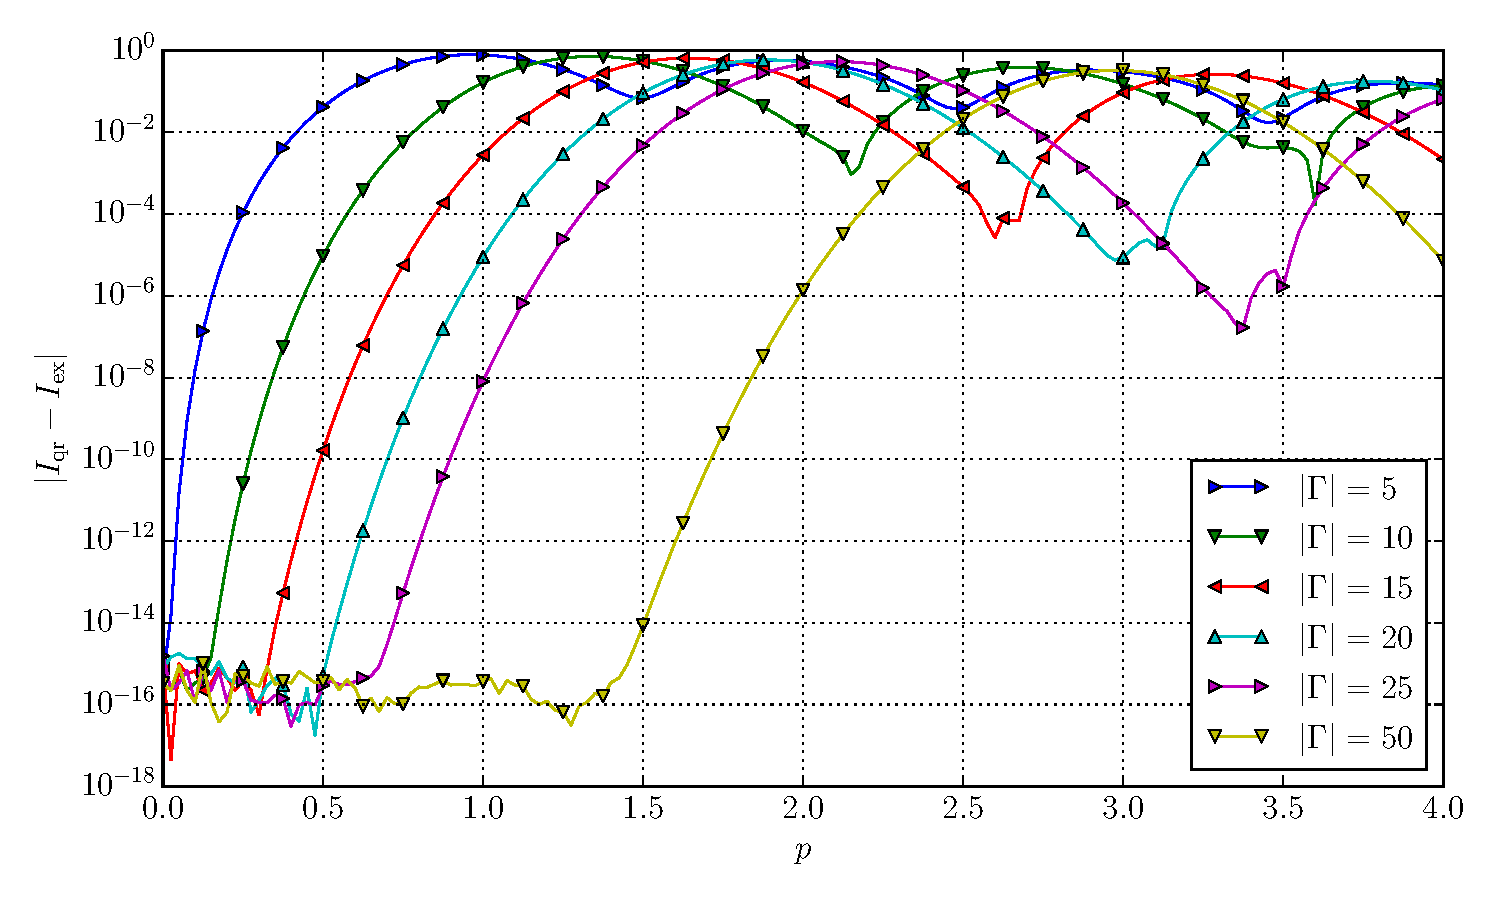
\includegraphics[width=\linewidth]{./plots/tp_2d_conv_p_(0,0)_(0,0)_err_qr.pdf}
    \caption{Absolute error of the Gauss-Hermite quadrature compared to the exact solution.}
    \label{fig:tp_2d_conv_p_00_00_err_qr}
  \end{subfigure}
  \begin{subfigure}{0.5\linewidth}
    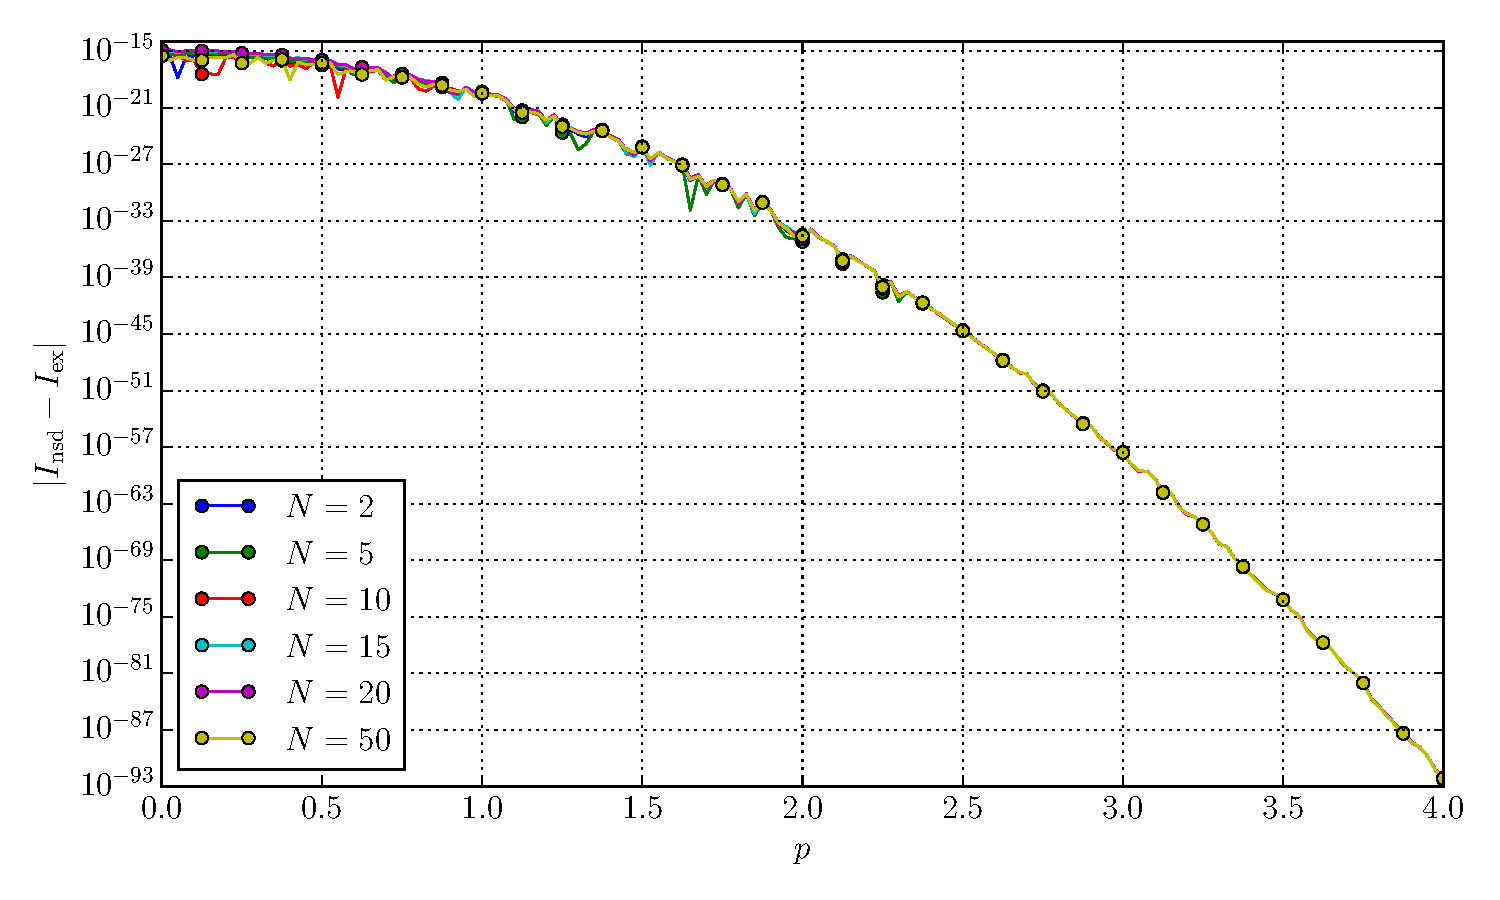
\includegraphics[width=\linewidth]{./plots/tp_2d_conv_p_(0,0)_(0,0)_err_nsd.pdf}
    \caption{Absolute error of the steepest descent method compared to the exact solution.}
    \label{fig:tp_2d_conv_p_00_00_err_nsd}
  \end{subfigure}
  \begin{subfigure}{0.5\linewidth}
    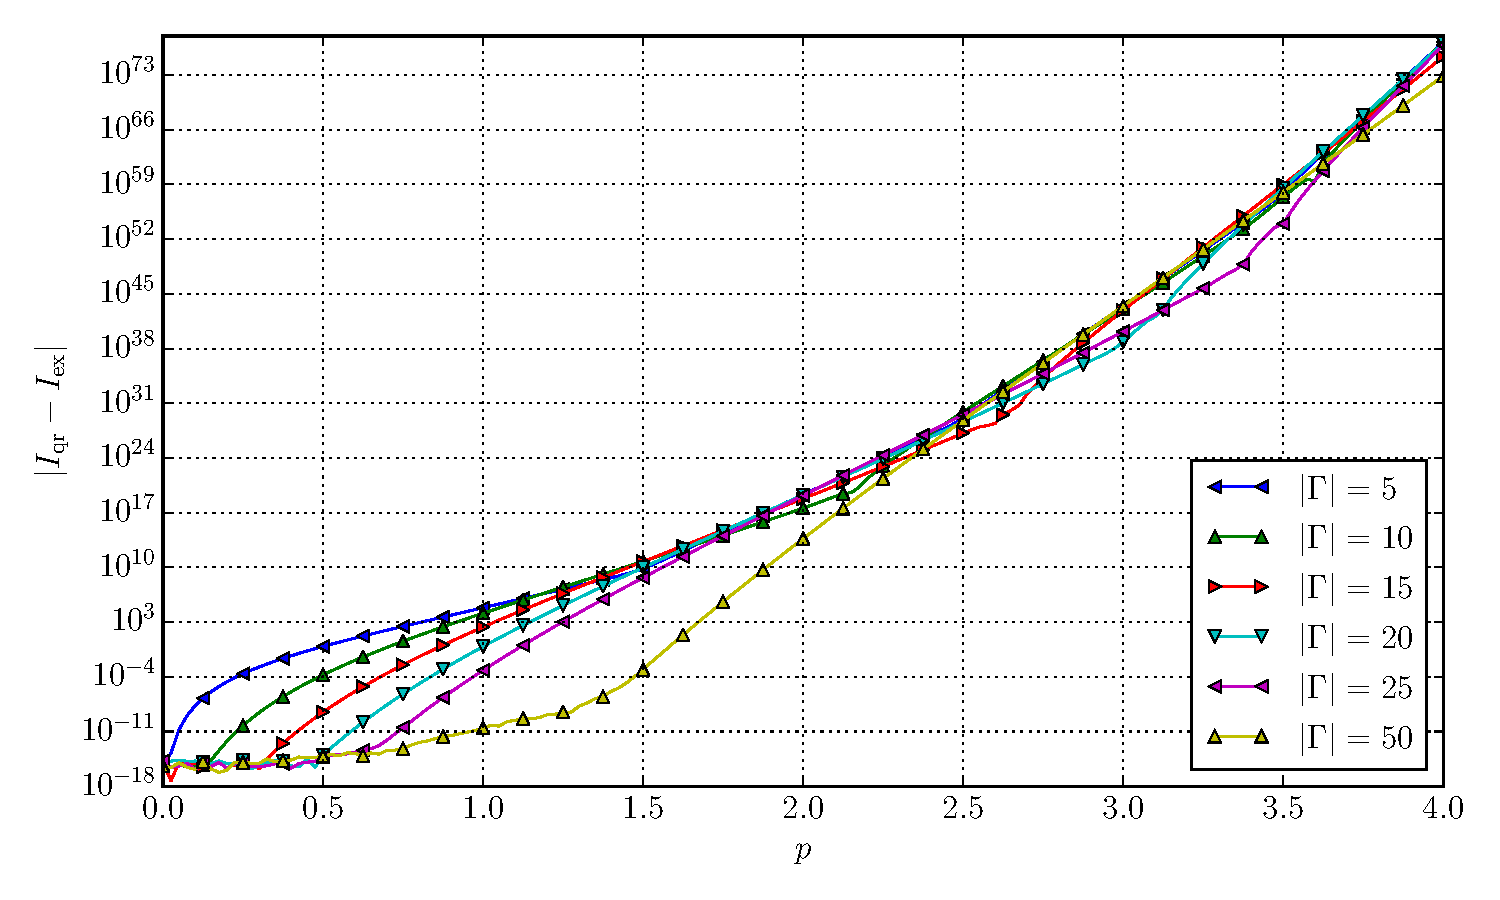
\includegraphics[width=\linewidth]{./plots/tp_2d_conv_p_(0,0)_(0,0)_err_rel_qr.pdf}
    \caption{Relative error of the Gauss-Hermite quadrature compared to the exact solution.}
    \label{fig:tp_2d_conv_p_00_00_err_rel_qr}
  \end{subfigure}
  \begin{subfigure}{0.5\linewidth}
    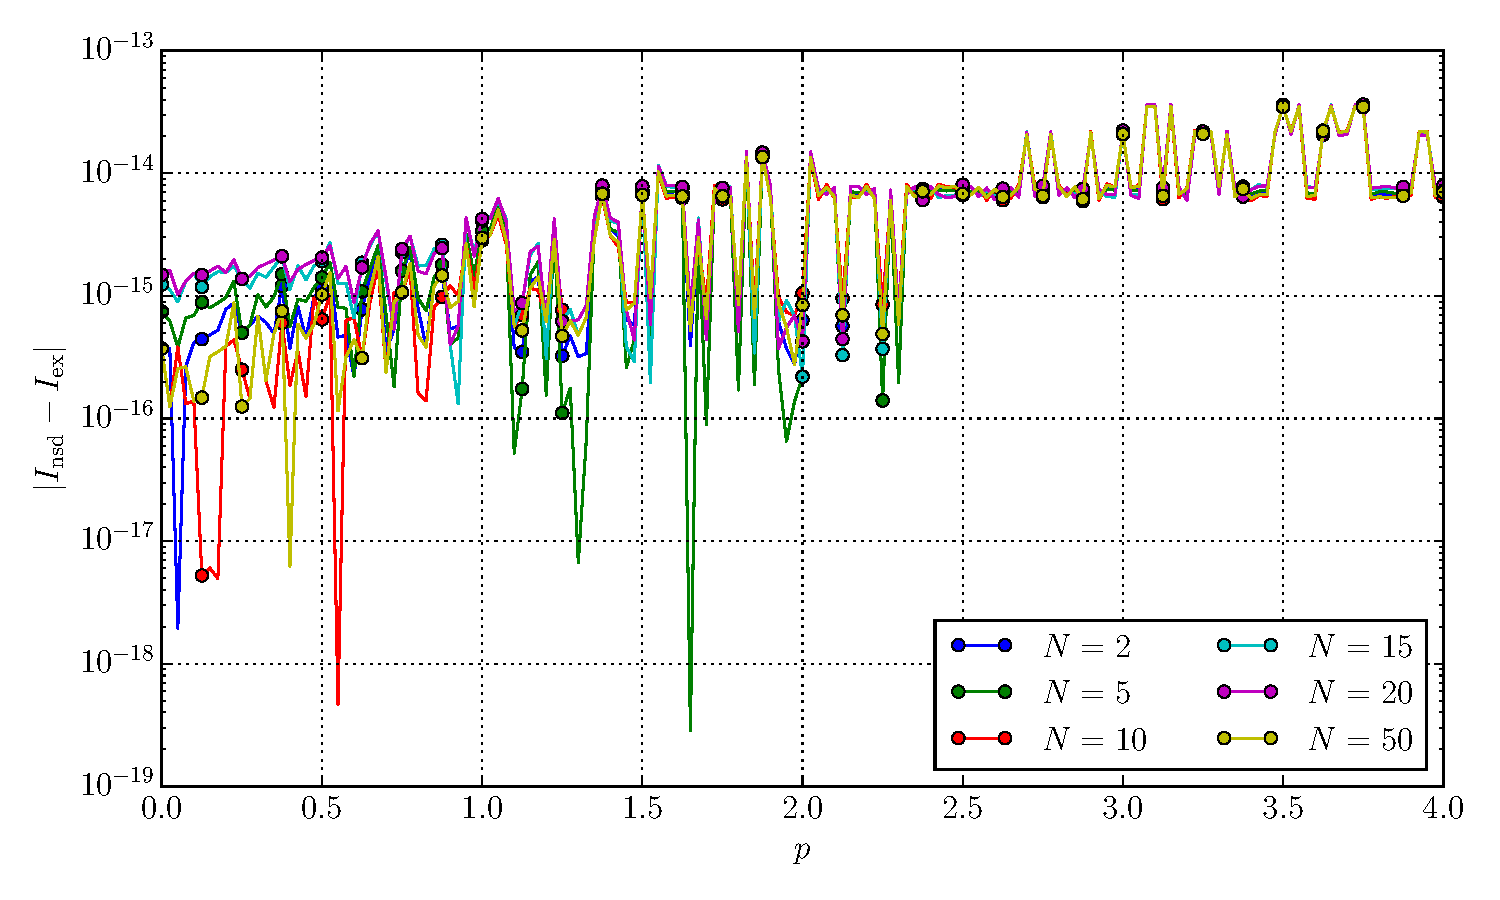
\includegraphics[width=\linewidth]{./plots/tp_2d_conv_p_(0,0)_(0,0)_err_rel_nsd.pdf}
    \caption{Relative error of the steepest descent method compared to the exact solution.}
    \label{fig:tp_2d_conv_p_00_00_err_rel_nsd}
  \end{subfigure}
  \label{fig:tp_2d_conv_p_00_00}
  \caption{Experiment with $\phi_{0,0}$ and $\phi_{0,0}^{\prime}$.
  The parameters are:
  $\vec{q} = (-0.1,  0.1)$,
  $\vec{p} = ( 1.0, -0.1)$,
  $\mat{Q} = \mat{1}$,
  $\mat{P} = \imath \mat{1}$
  and
  $\vec{q}^\prime = ( 0.1, 0.1)$,
  $\vec{p}^\prime = (-1.0, 0.1)$,
  $\mat{Q}^\prime = \mat{1}$,
  $\mat{P}^\prime = \imath \mat{1}$
  with $\varepsilon=0.3$.}
\end{figure}

\begin{figure}
  \begin{subfigure}{0.5\linewidth}
    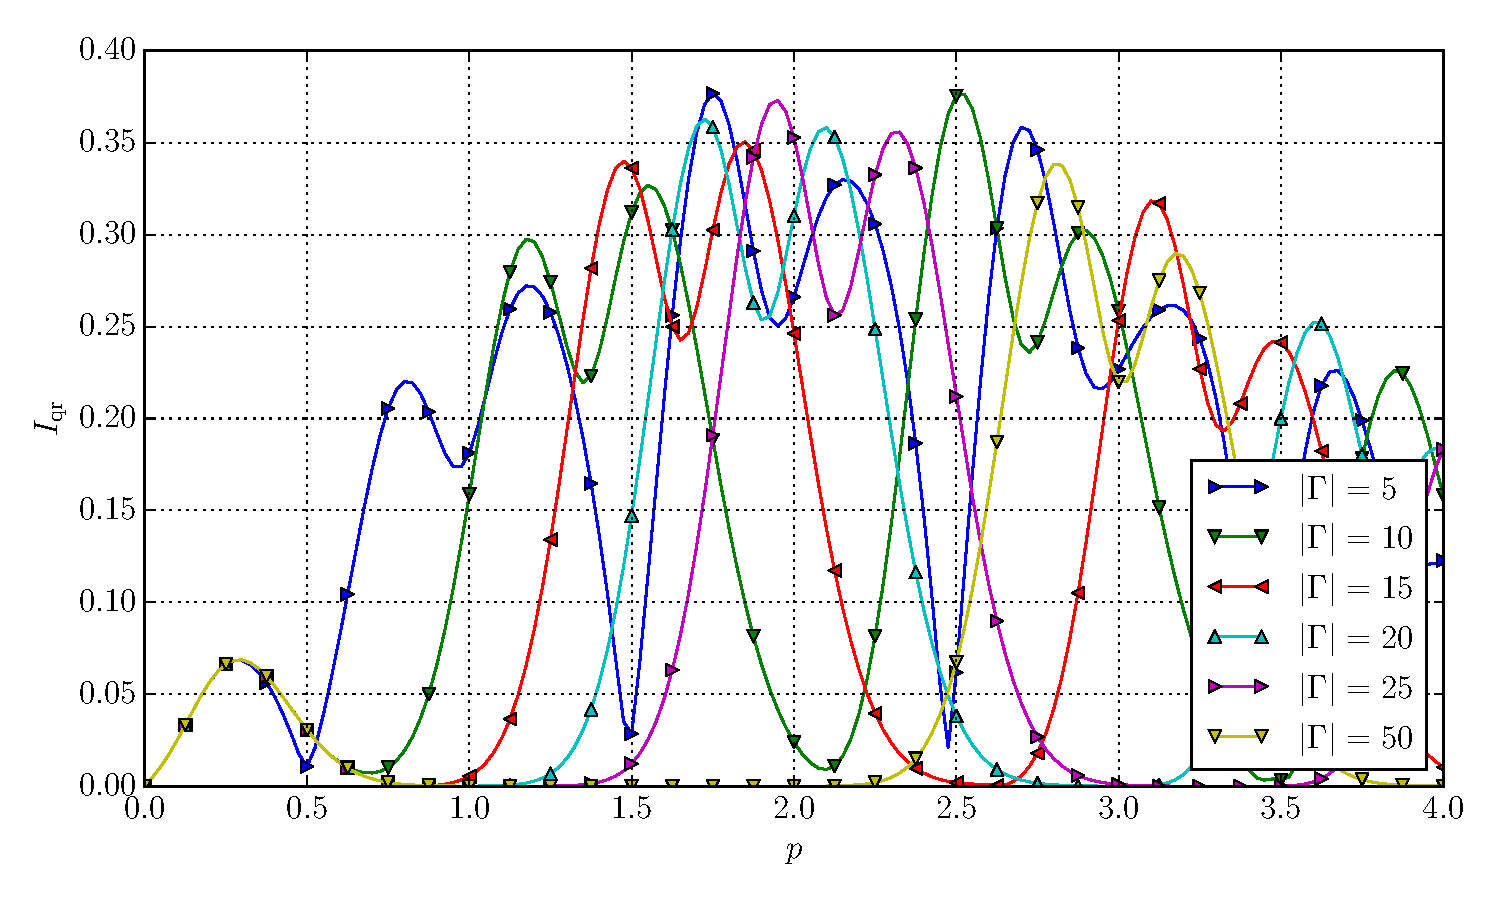
\includegraphics[width=\linewidth]{./plots/tp_2d_conv_p_(0,1)_(1,0)_val_qr.pdf}
    \caption{Gauss-Hermite quadrature with $|\Gamma|$ nodes.}
    \label{fig:tp_2d_conv_p_01_10_val_qr}
  \end{subfigure}
  \begin{subfigure}{0.5\linewidth}
    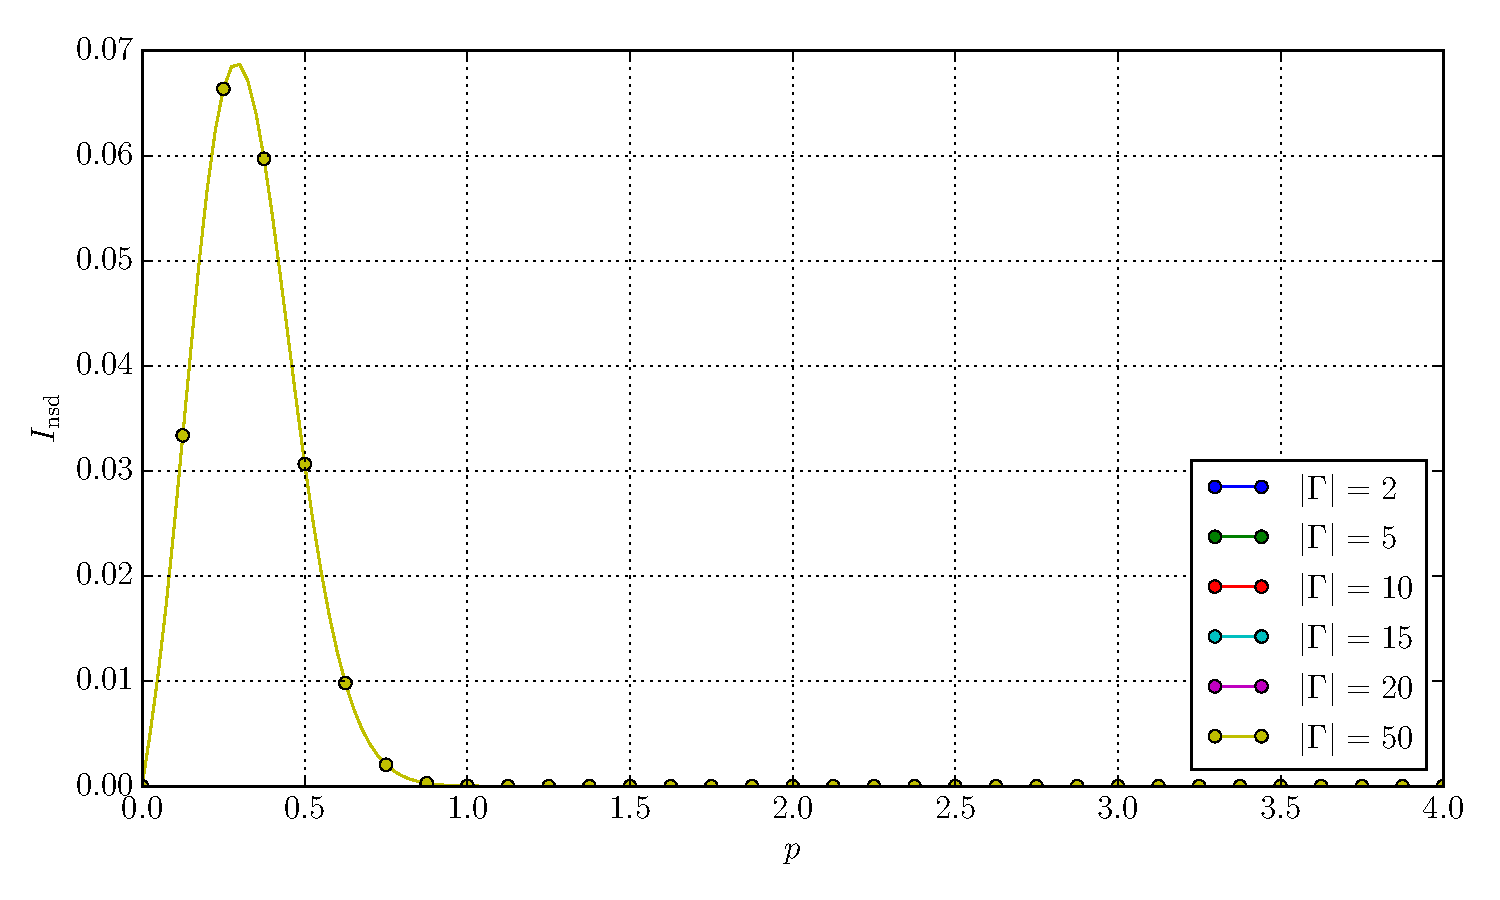
\includegraphics[width=\linewidth]{./plots/tp_2d_conv_p_(0,1)_(1,0)_val_nsd.pdf}
    \caption{Steepest descent transformation and quadrature with $|\Gamma|$ nodes.}
    \label{fig:tp_2d_conv_p_01_10_val_nsd}
  \end{subfigure} \\
  \begin{subfigure}{0.5\linewidth}
    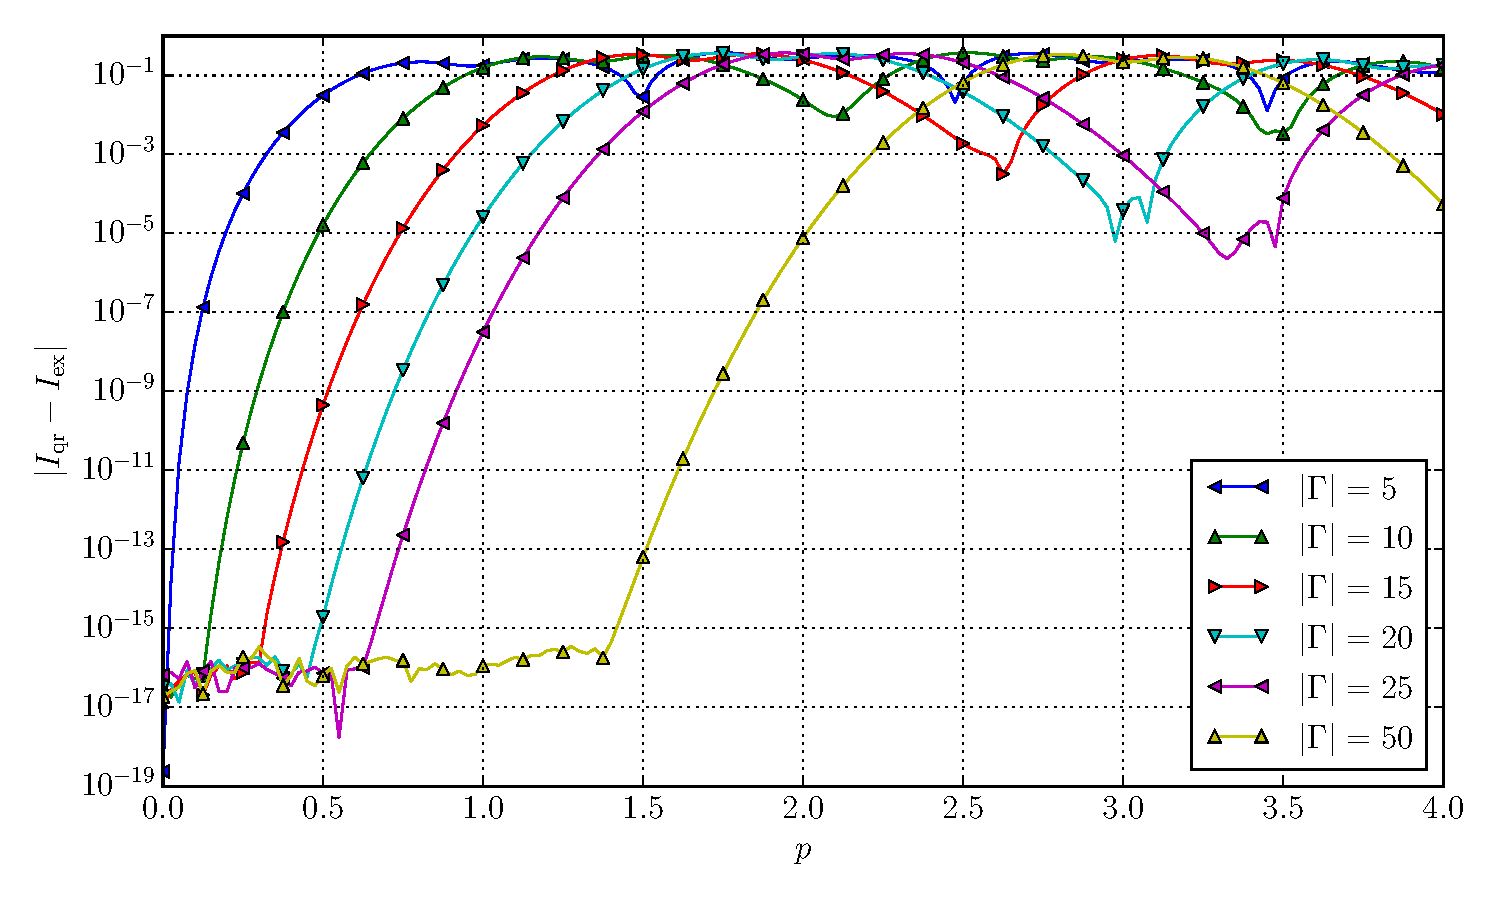
\includegraphics[width=\linewidth]{./plots/tp_2d_conv_p_(0,1)_(1,0)_err_qr.pdf}
    \caption{Absolute error of the Gauss-Hermite quadrature compared to the exact solution.}
    \label{fig:tp_2d_conv_p_01_10_err_qr}
  \end{subfigure}
  \begin{subfigure}{0.5\linewidth}
    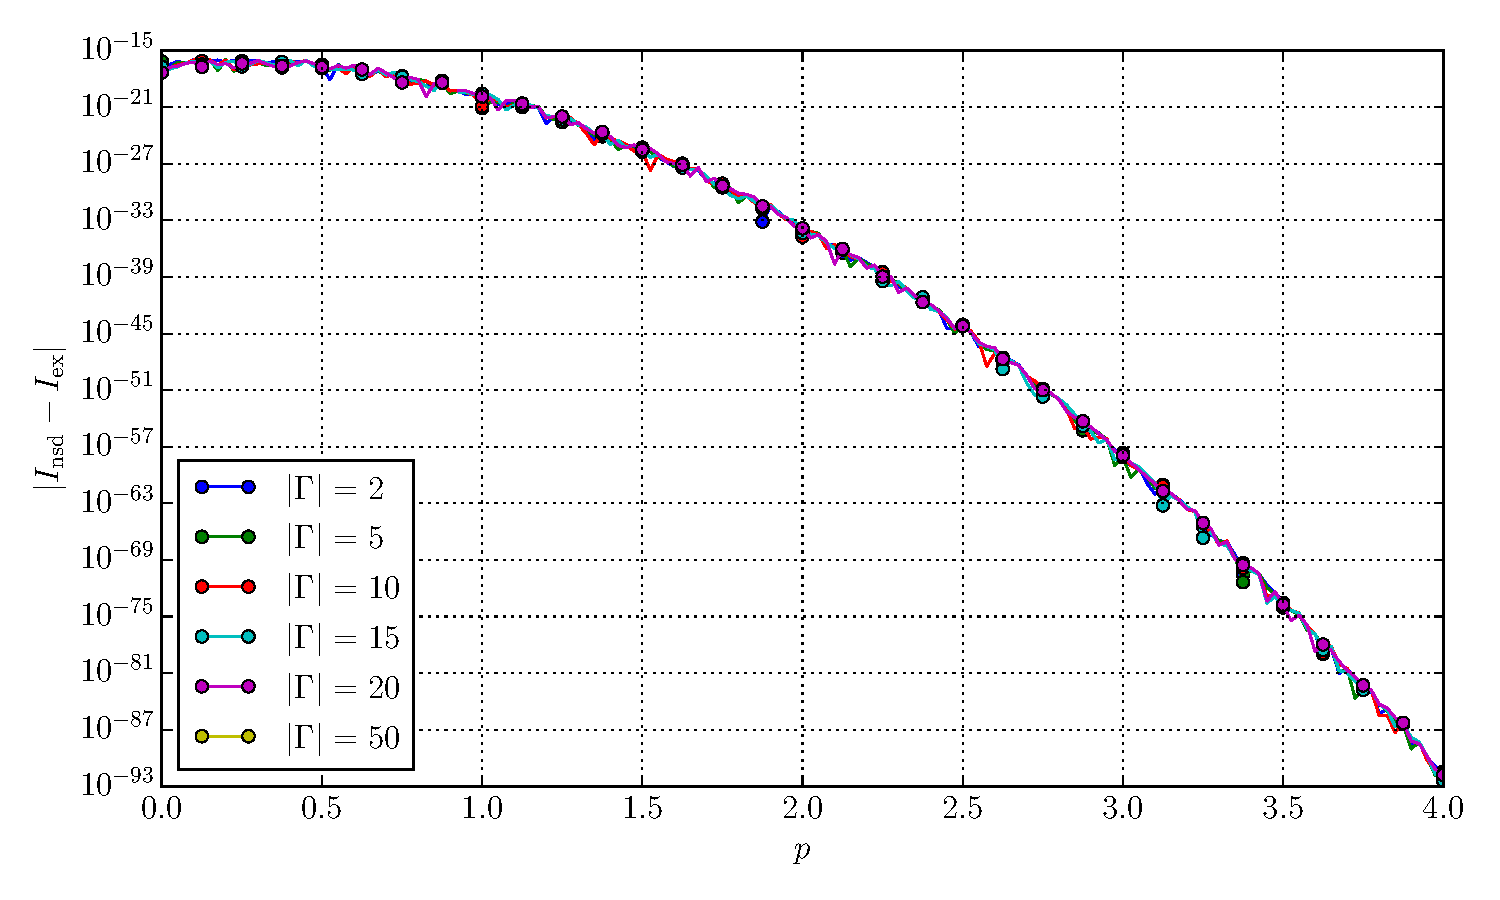
\includegraphics[width=\linewidth]{./plots/tp_2d_conv_p_(0,1)_(1,0)_err_nsd.pdf}
    \caption{Absolute error of the steepest descent method compared to the exact solution.}
    \label{fig:tp_2d_conv_p_01_10_err_nsd}
  \end{subfigure}
  \begin{subfigure}{0.5\linewidth}
    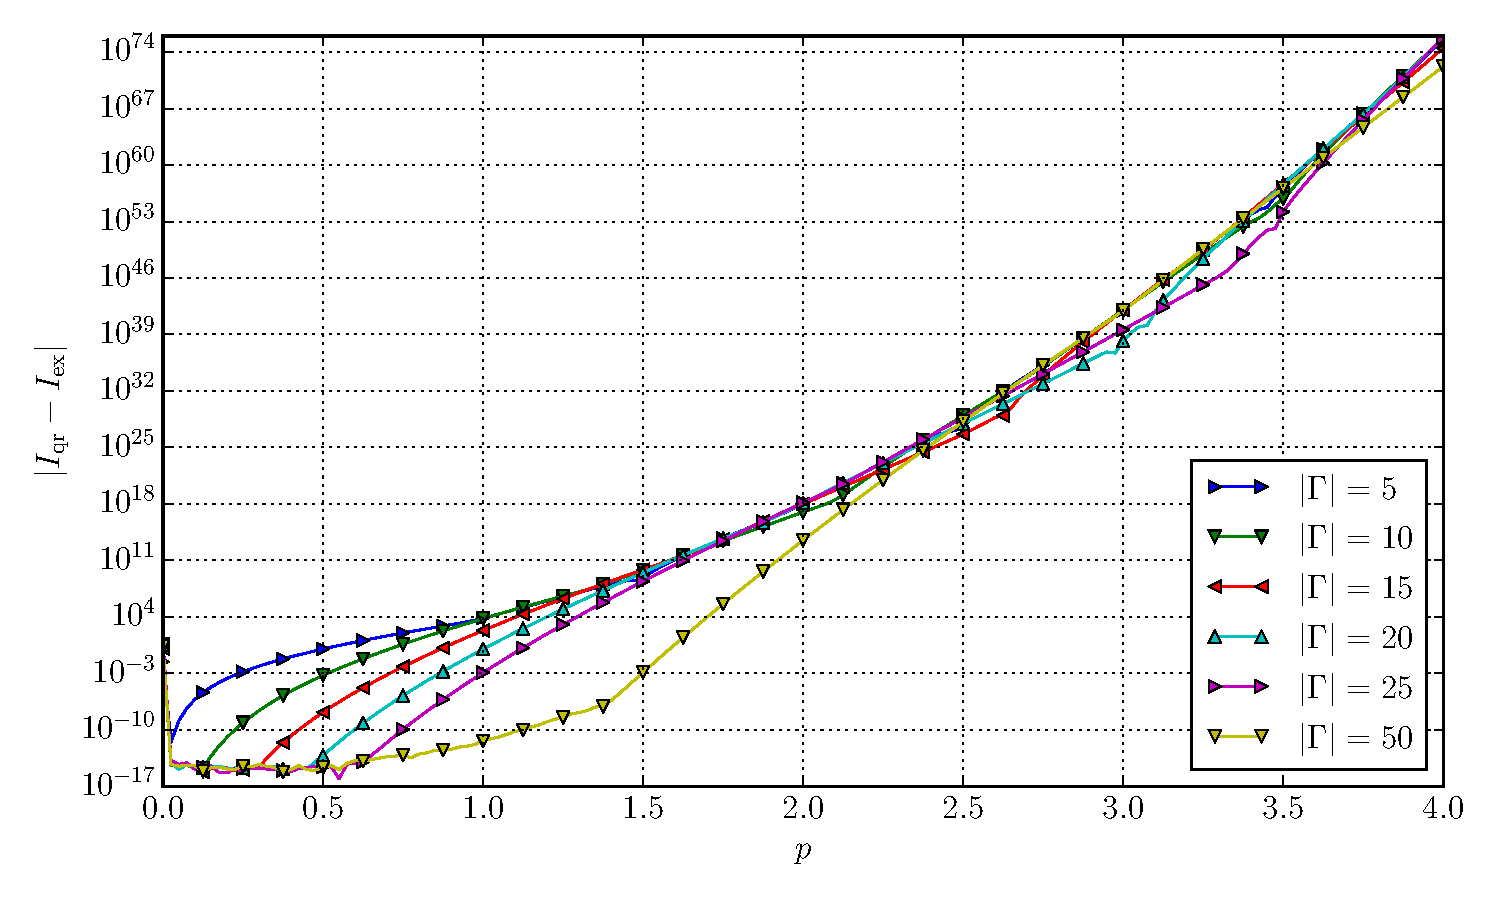
\includegraphics[width=\linewidth]{./plots/tp_2d_conv_p_(0,1)_(1,0)_err_rel_qr.pdf}
    \caption{Relative error of the Gauss-Hermite quadrature compared to the exact solution.}
    \label{fig:tp_2d_conv_p_01_10_err_qr}
  \end{subfigure}
  \begin{subfigure}{0.5\linewidth}
    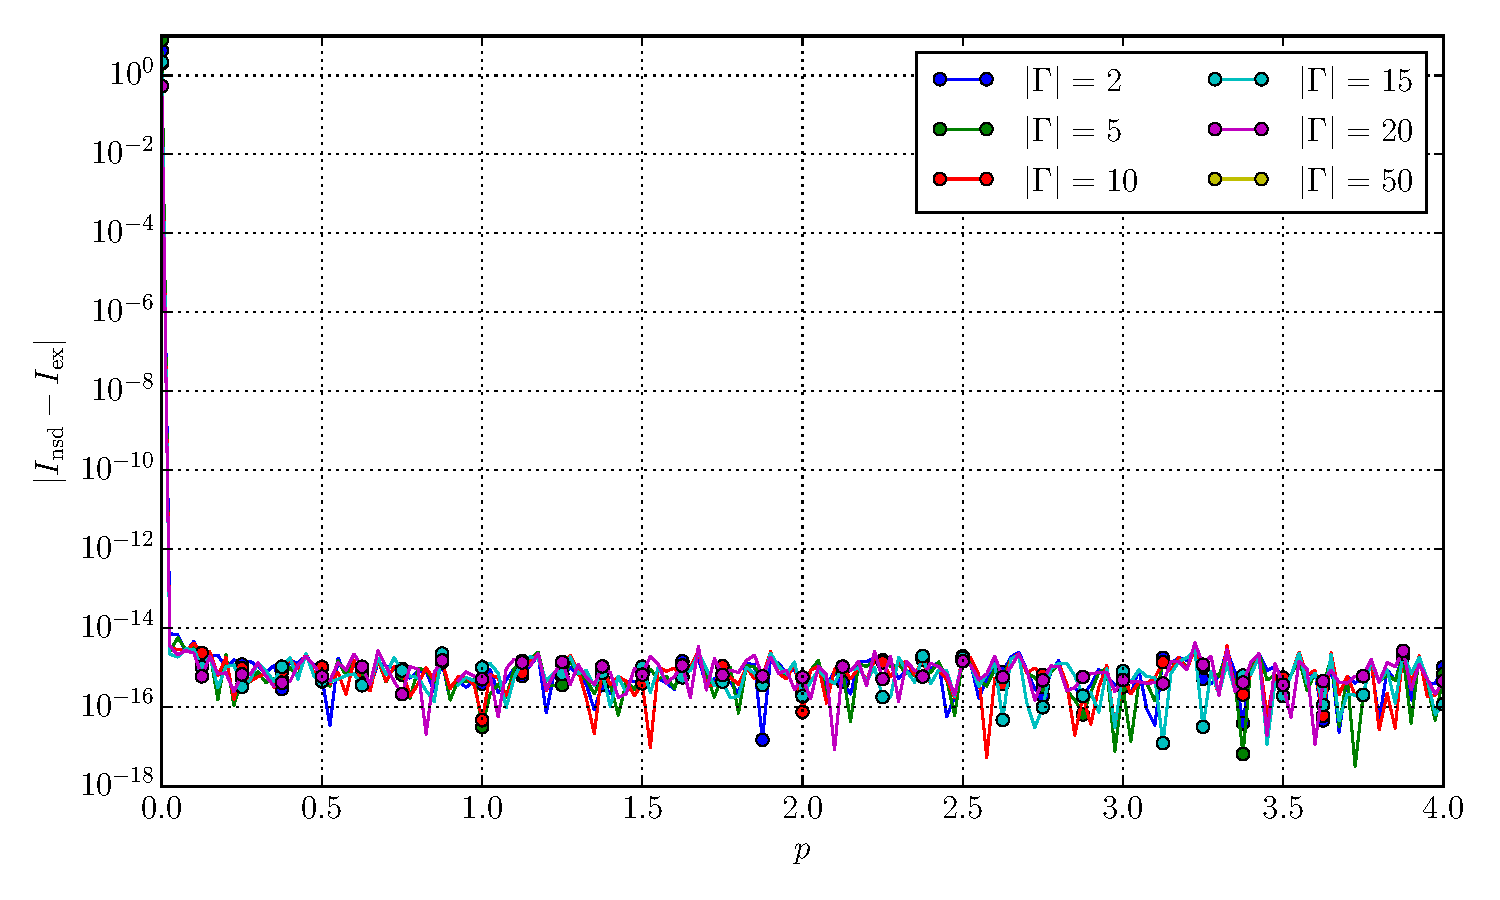
\includegraphics[width=\linewidth]{./plots/tp_2d_conv_p_(0,1)_(1,0)_err_rel_nsd.pdf}
    \caption{Relative error of the steepest descent method compared to the exact solution.}
    \label{fig:tp_2d_conv_p_01_10_err_nsd}
  \end{subfigure}
  \label{fig:tp_2d_conv_p_01_10}
  \caption{Experiment with $\phi_{0,1}$ and $\phi_{1,0}^{\prime}$.
  The parameters are:
  $\vec{q} = (-0.1,  0.1)$,
  $\vec{p} = ( 1.0, -0.1)$,
  $\mat{Q} = \mat{1}$,
  $\mat{P} = \imath \mat{1}$
  and
  $\vec{q}^\prime = ( 0.1, 0.1)$,
  $\vec{p}^\prime = (-1.0, 0.1)$,
  $\mat{Q}^\prime = \mat{1}$,
  $\mat{P}^\prime = \imath \mat{1}$
  with $\varepsilon=0.3$.}
\end{figure}

\begin{figure}
  \begin{subfigure}{0.5\linewidth}
    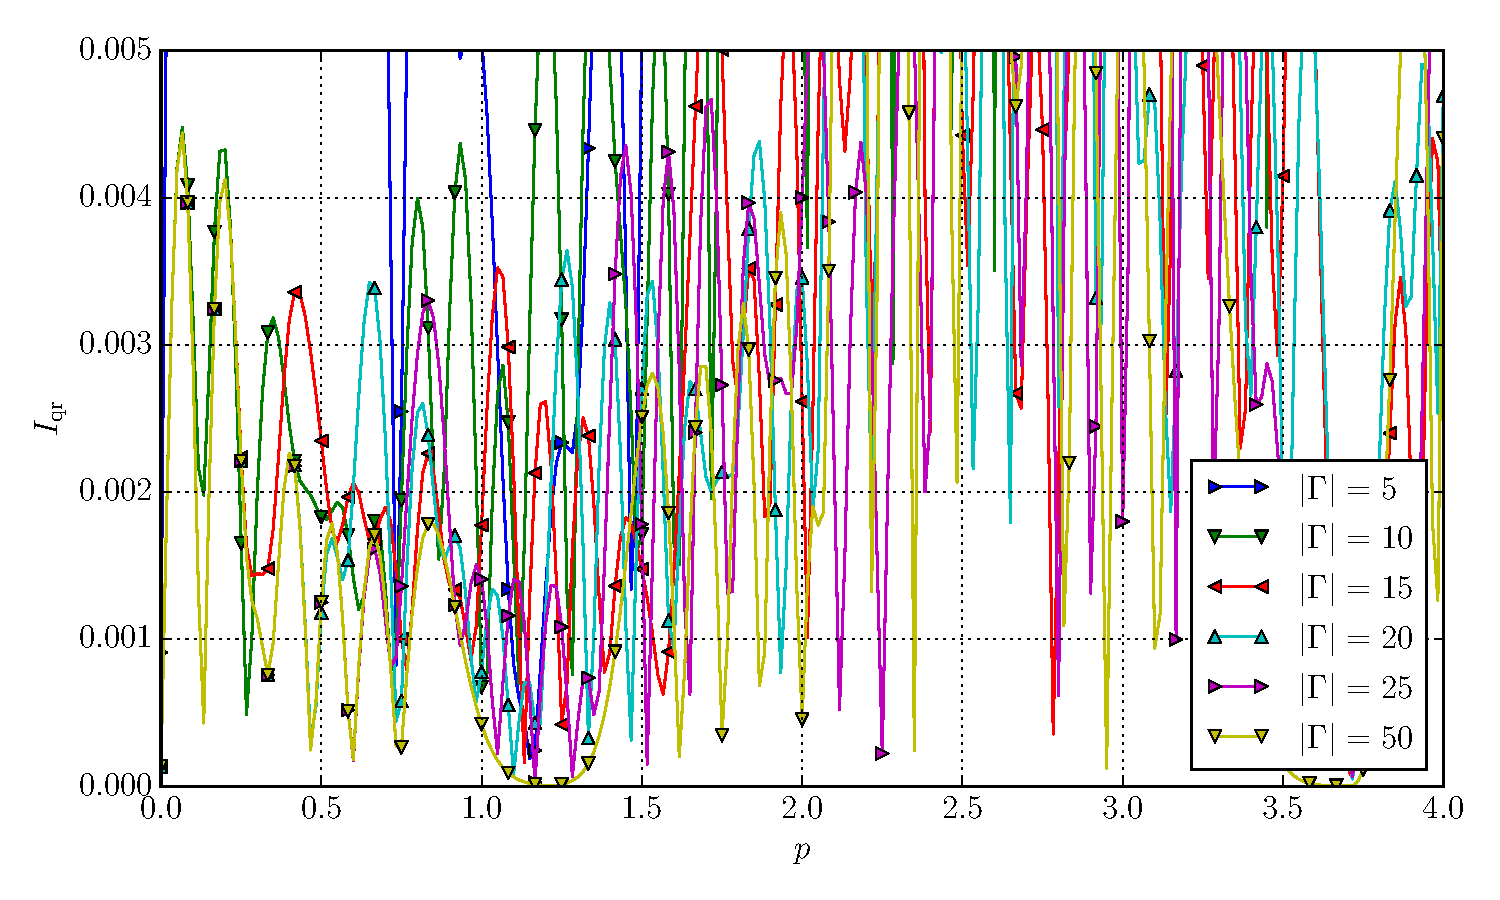
\includegraphics[width=\linewidth]{./plots/tp_2d_conv_p_(8,8)_(8,8)_val_qr.pdf}
    \caption{Gauss-Hermite quadrature with $|\Gamma|$ nodes.}
    \label{fig:tp_2d_conv_p_88_88_val_qr}
  \end{subfigure}
  \begin{subfigure}{0.5\linewidth}
    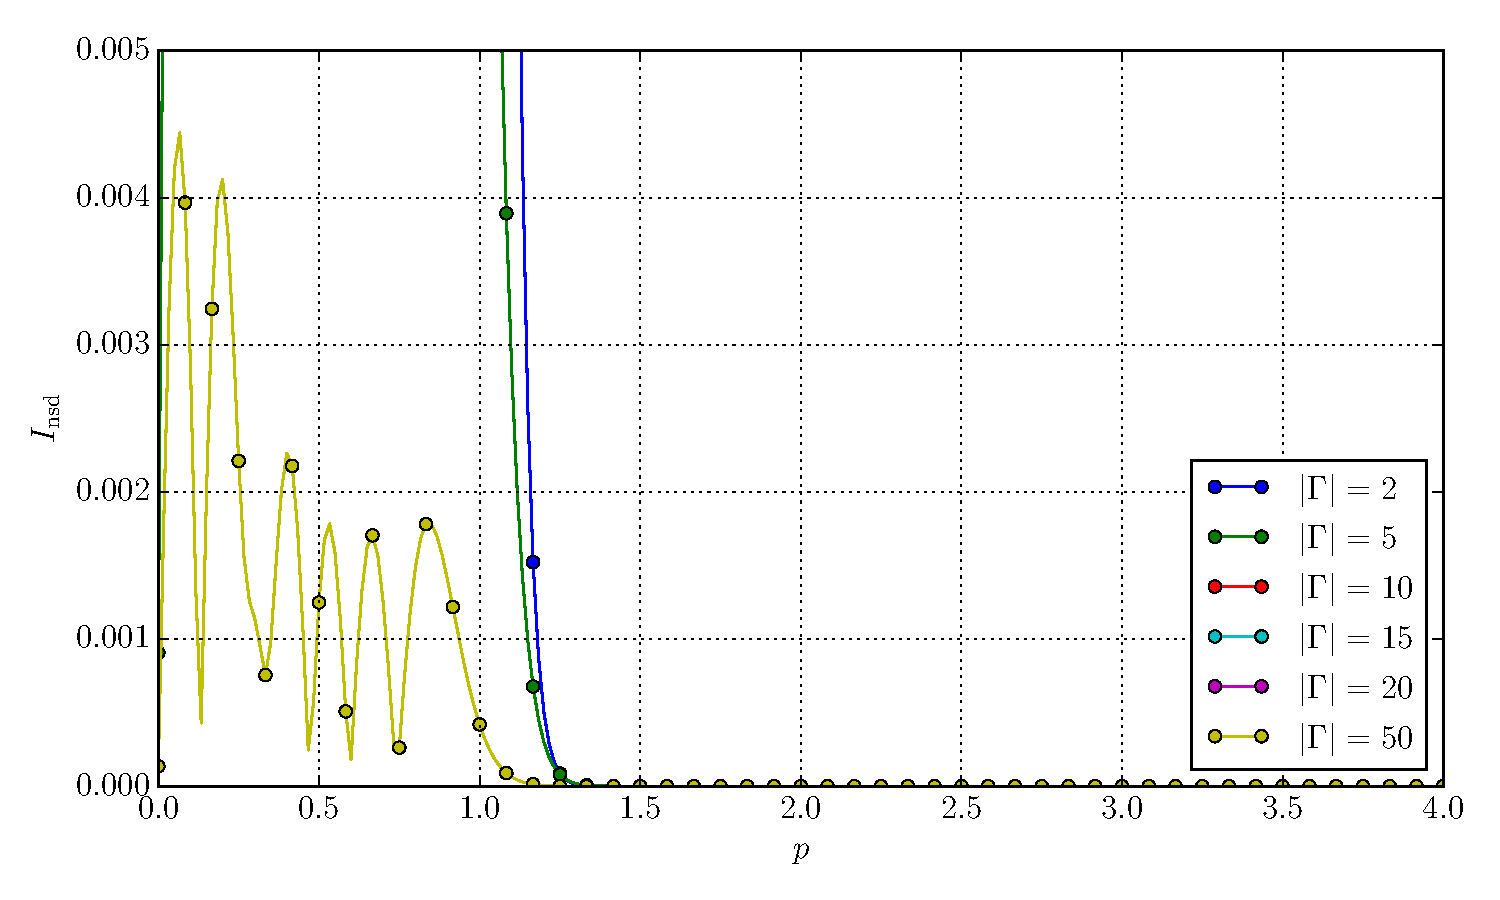
\includegraphics[width=\linewidth]{./plots/tp_2d_conv_p_(8,8)_(8,8)_val_nsd.pdf}
    \caption{Steepest descent transformation and quadrature with $|\Gamma|$ nodes.}
    \label{fig:tp_2d_conv_p_88_88_val_nsd}
  \end{subfigure} \\
  \begin{subfigure}{0.5\linewidth}
    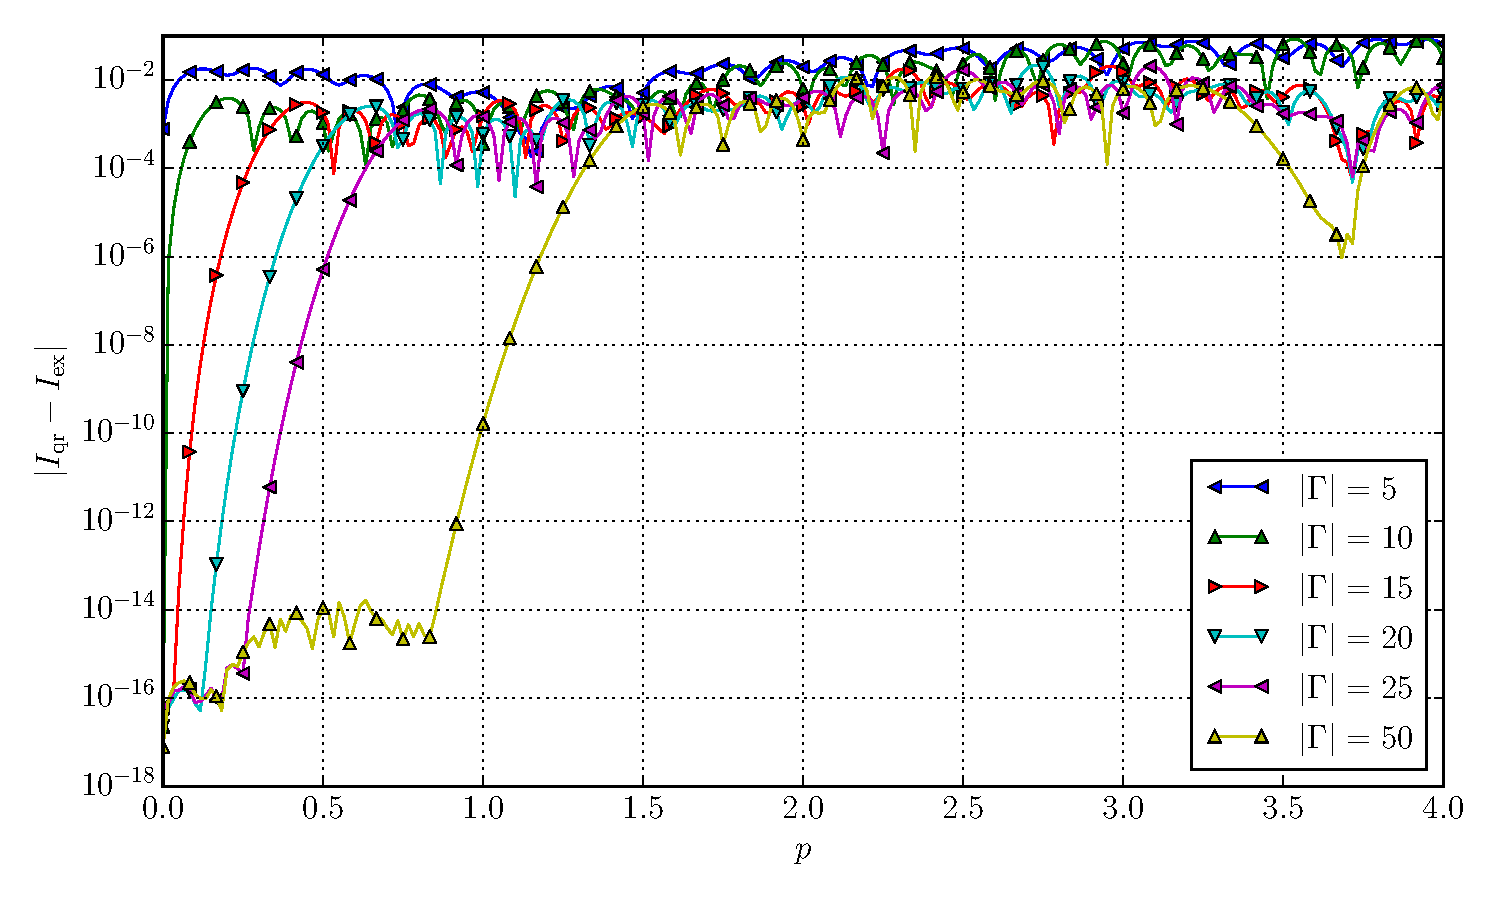
\includegraphics[width=\linewidth]{./plots/tp_2d_conv_p_(8,8)_(8,8)_err_qr.pdf}
    \caption{Absolute error of the Gauss-Hermite quadrature compared to the exact solution.}
    \label{fig:tp_2d_conv_p_88_88_err_qr}
  \end{subfigure}
  \begin{subfigure}{0.5\linewidth}
    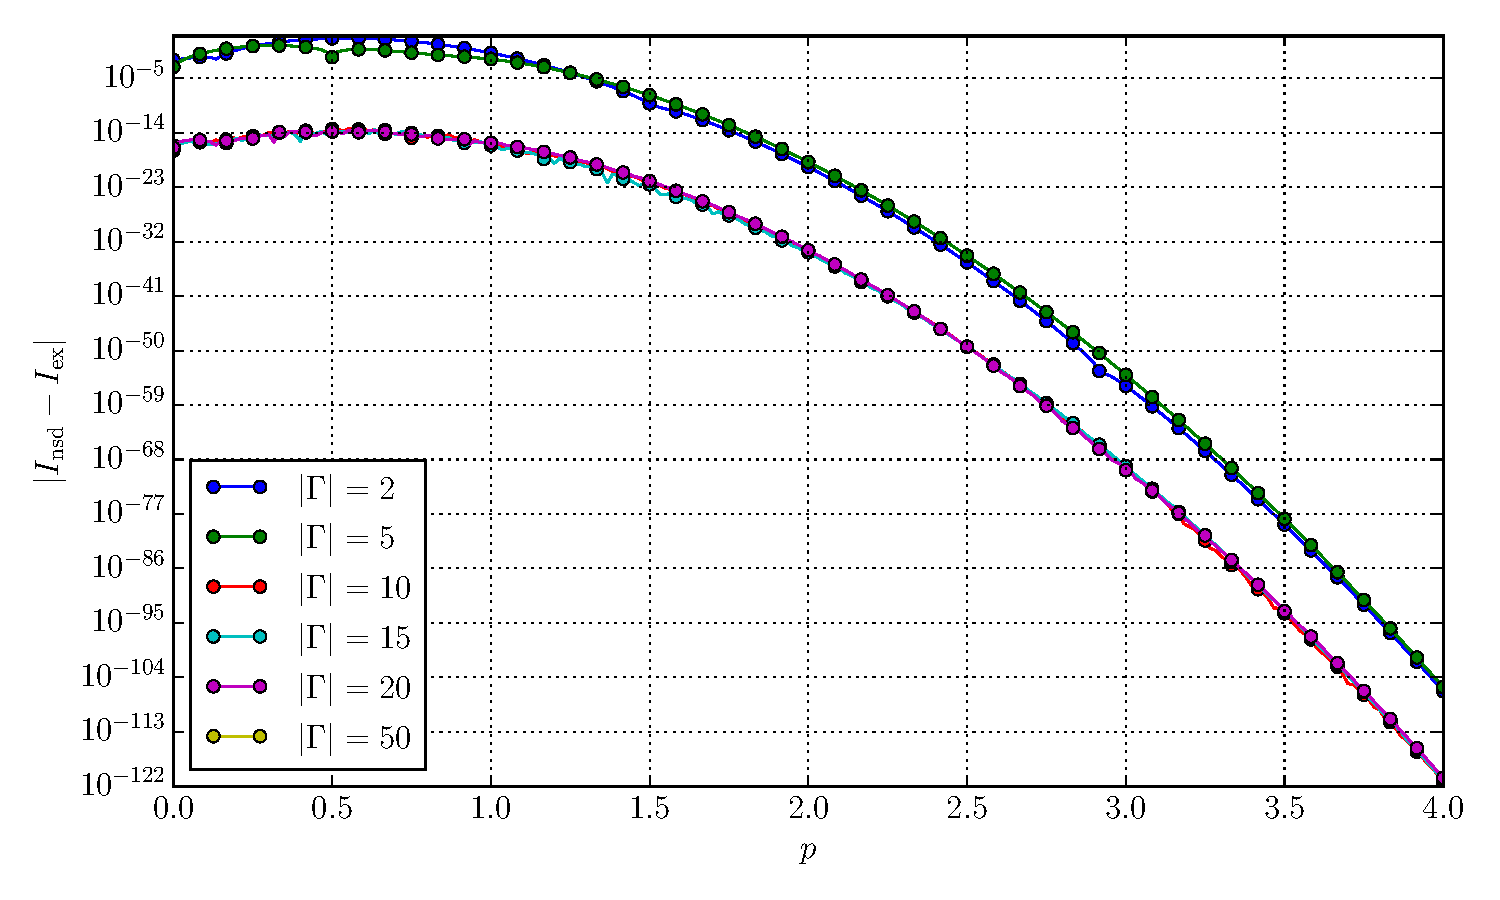
\includegraphics[width=\linewidth]{./plots/tp_2d_conv_p_(8,8)_(8,8)_err_nsd.pdf}
    \caption{Absolute error of the steepest descent method compared to the exact solution.}
    \label{fig:tp_2d_conv_p_88_88_err_nsd}
  \end{subfigure}
  \begin{subfigure}{0.5\linewidth}
    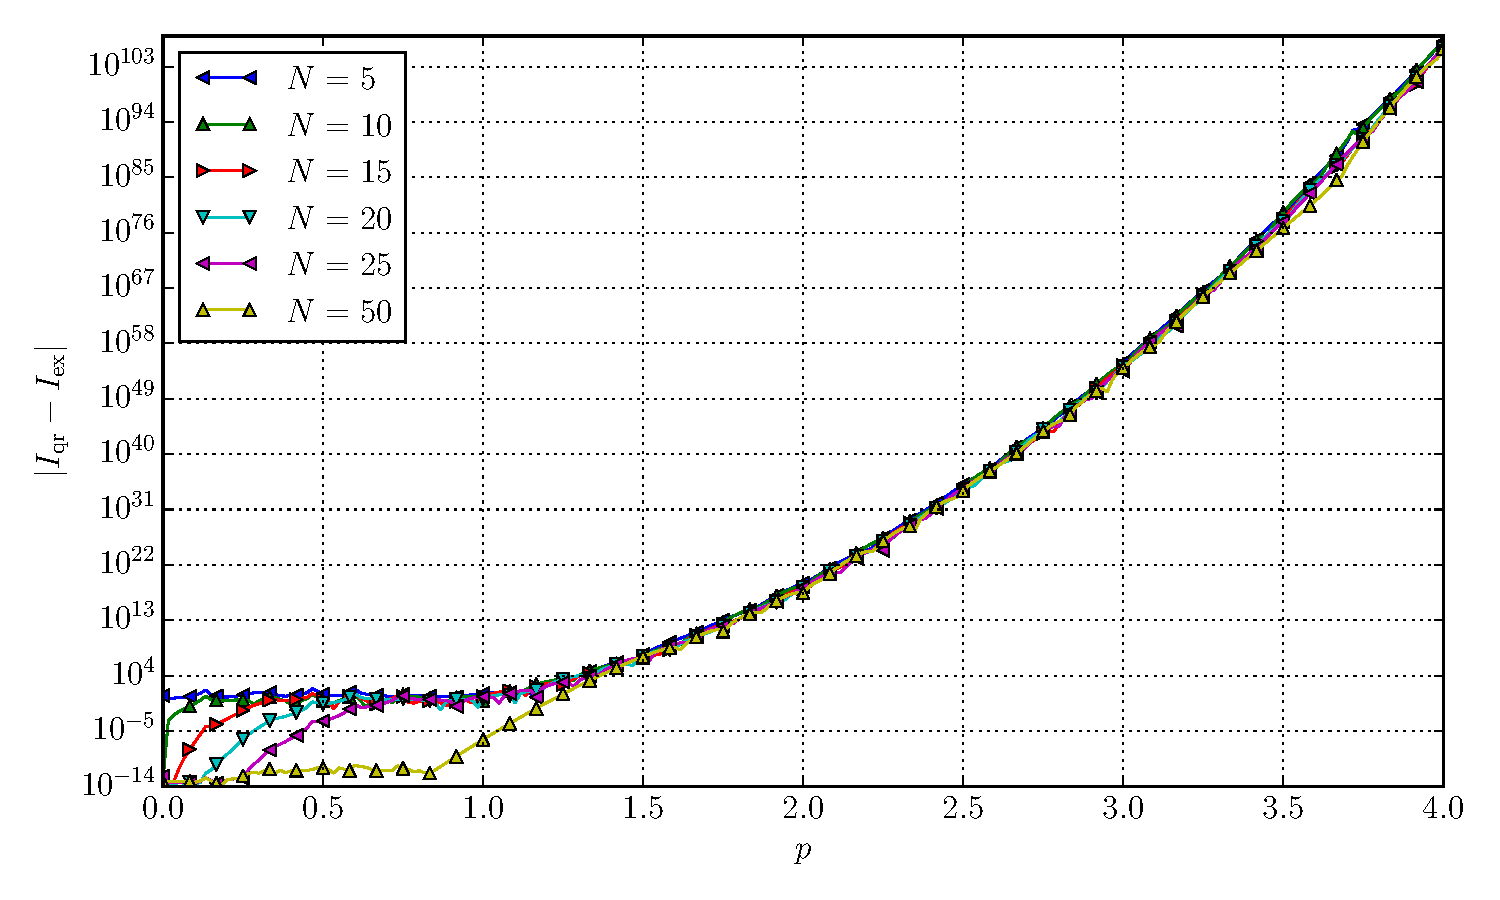
\includegraphics[width=\linewidth]{./plots/tp_2d_conv_p_(8,8)_(8,8)_err_rel_qr.pdf}
    \caption{Relative error of the Gauss-Hermite quadrature compared to the exact solution.}
    \label{fig:tp_2d_conv_p_88_88_err_qr}
  \end{subfigure}
  \begin{subfigure}{0.5\linewidth}
    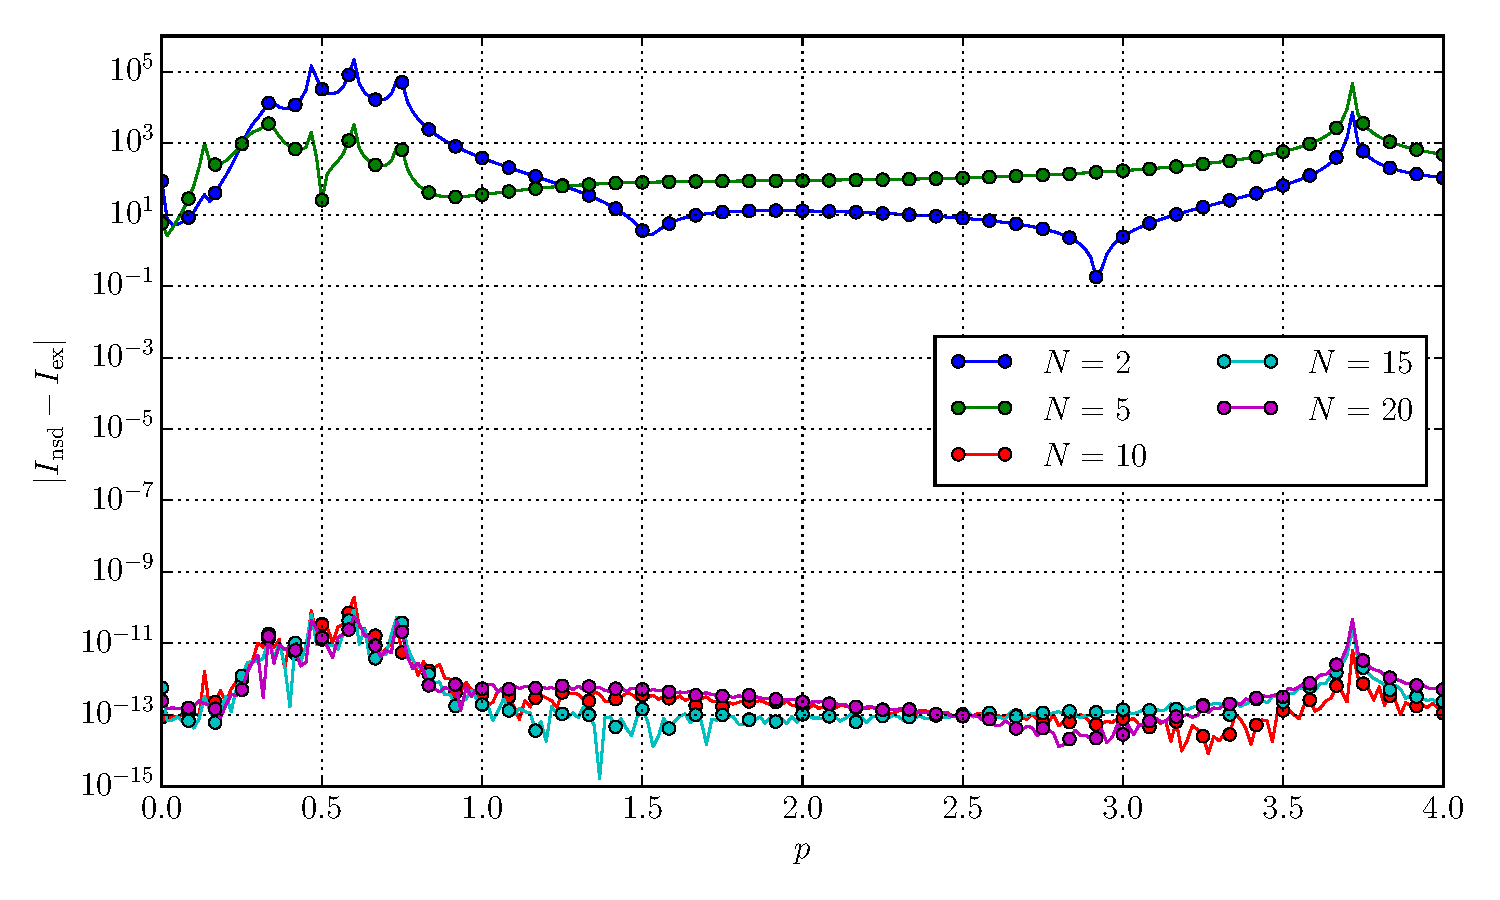
\includegraphics[width=\linewidth]{./plots/tp_2d_conv_p_(8,8)_(8,8)_err_rel_nsd.pdf}
    \caption{Relative error of the steepest descent method compared to the exact solution.}
    \label{fig:tp_2d_conv_p_88_88_err_nsd}
  \end{subfigure}
  \label{fig:tp_2d_conv_p_88_88}
  \caption{Experiment with $\phi_{8,8}$ and $\phi_{8,8}^{\prime}$.
  The parameters are:
  $\vec{q} = (-0.1,  0.1)$,
  $\vec{p} = ( 1.0, -0.1)$,
  $\mat{Q} = ( 1.0,       0; 0, 1.0)$,
  $\mat{P} = ( 1.0\imath, 0; 0, 1.0\imath)$
  and
  $\vec{q}^\prime = ( 0.1, 0.1)$,
  $\vec{p}^\prime = (-1.0, 0.1)$,
  $\mat{Q}^\prime = ( 2.0,       0; 0, 0.5)$,
  $\mat{P}^\prime = ( 0.5\imath, 0; 0, 2.0\imath)$
  with $\varepsilon=0.3$.}
\end{figure}

\begin{figure}
  \begin{subfigure}{0.5\linewidth}
    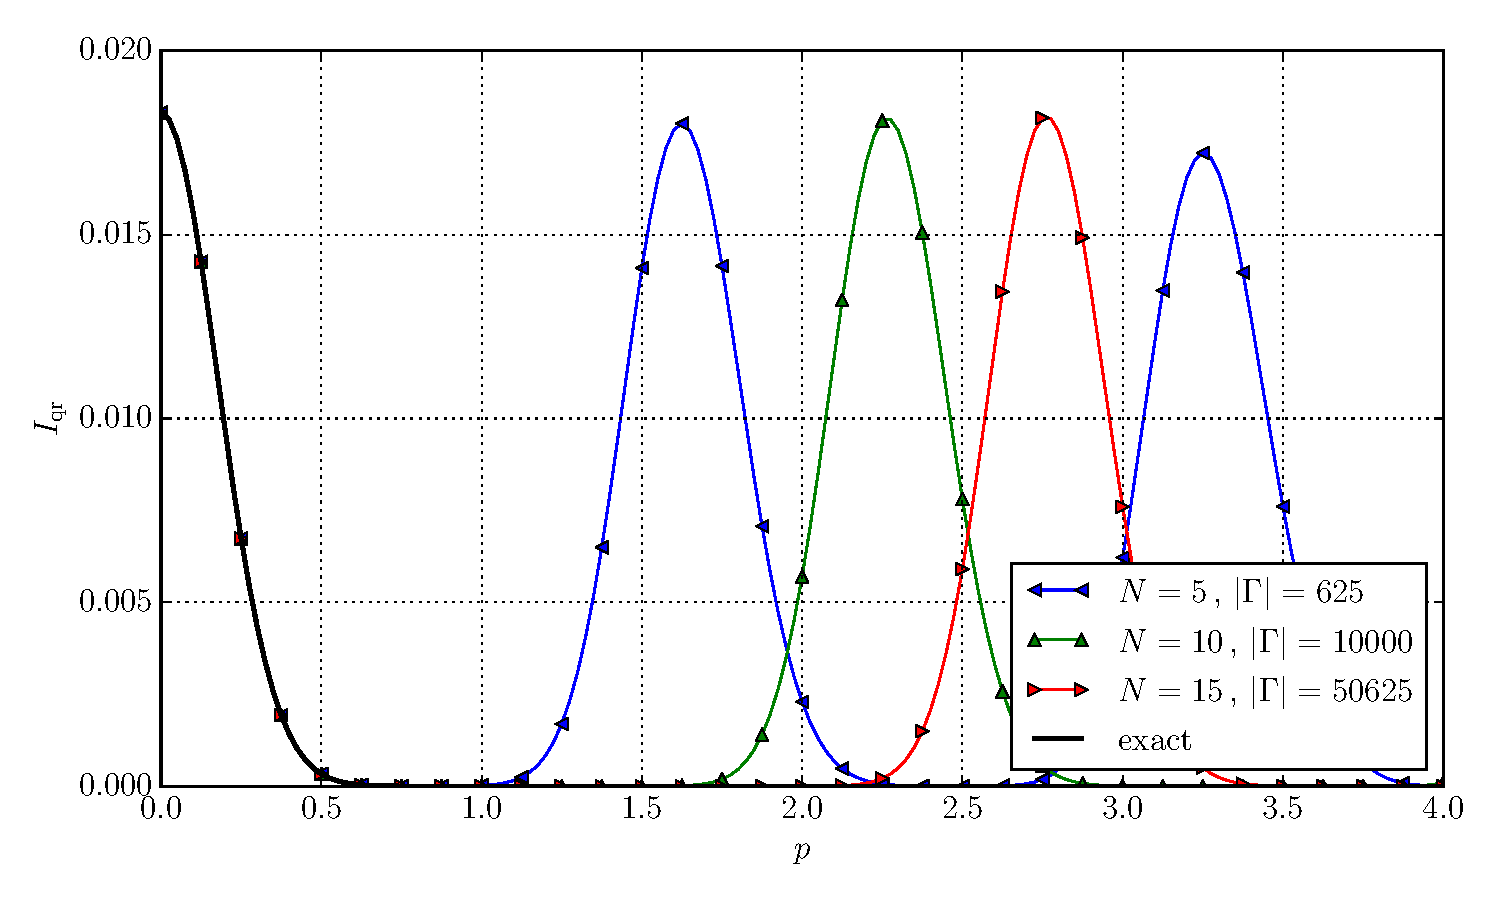
\includegraphics[width=\linewidth]{./plots/tp_4d_conv_p_(0,0,0,0)_(0,0,0,0)_val_qr.pdf}
    \caption{Gauss-Hermite quadrature with $|\Gamma|$ nodes.}
    \label{fig:tp_4d_conv_p_0000_0000_val_qr}
  \end{subfigure}
  \begin{subfigure}{0.5\linewidth}
    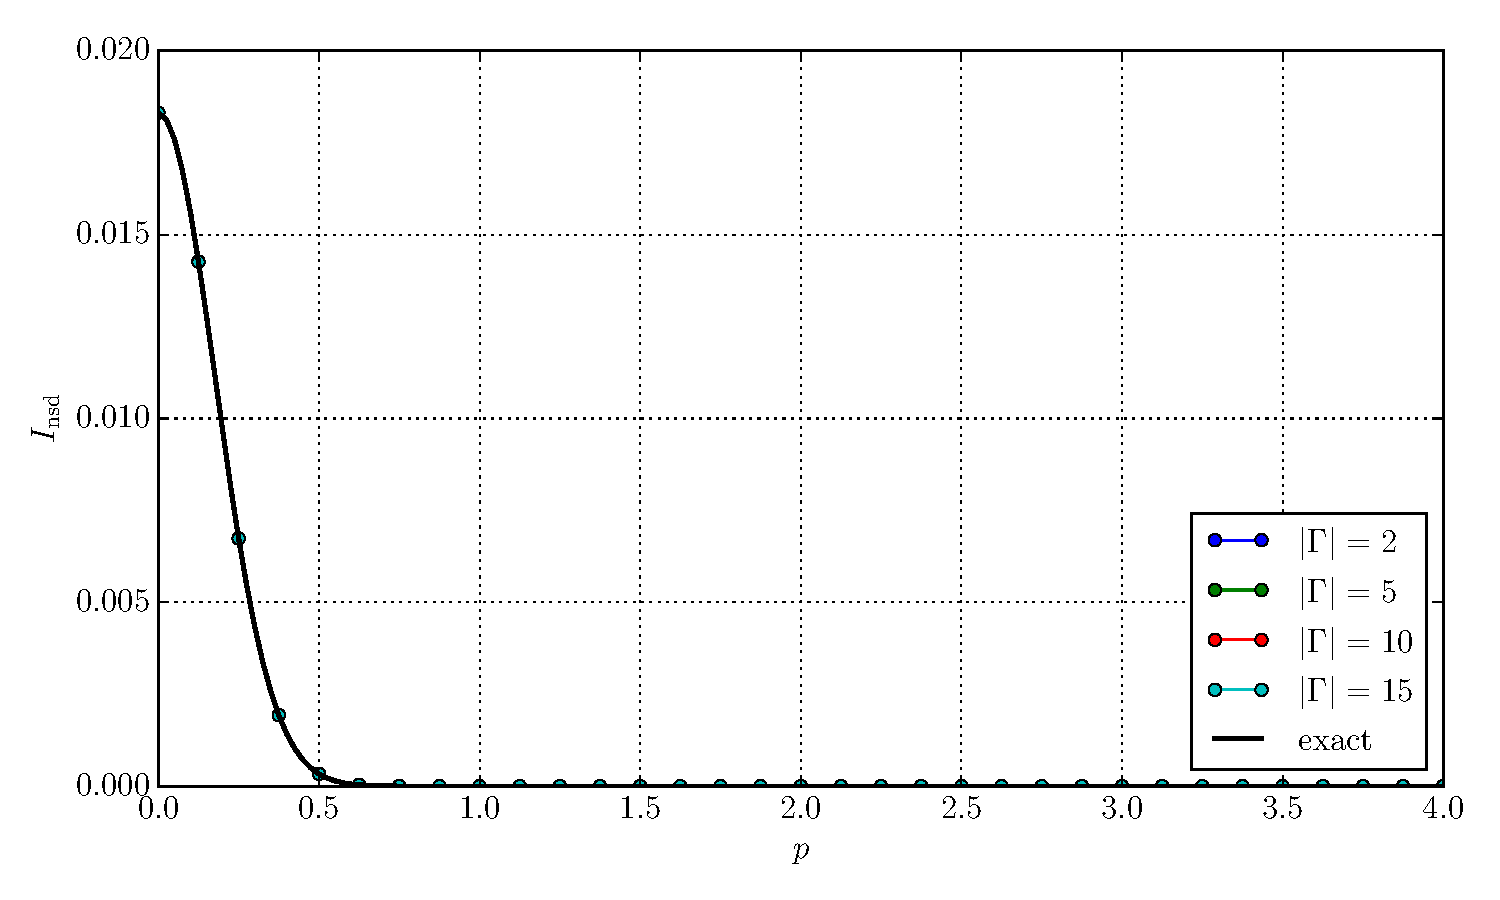
\includegraphics[width=\linewidth]{./plots/tp_4d_conv_p_(0,0,0,0)_(0,0,0,0)_val_nsd.pdf}
    \caption{Steepest descent transformation and quadrature with $|\Gamma|$ nodes.}
    \label{fig:tp_4d_conv_p_0000_0000_val_nsd}
  \end{subfigure} \\
  \begin{subfigure}{0.5\linewidth}
    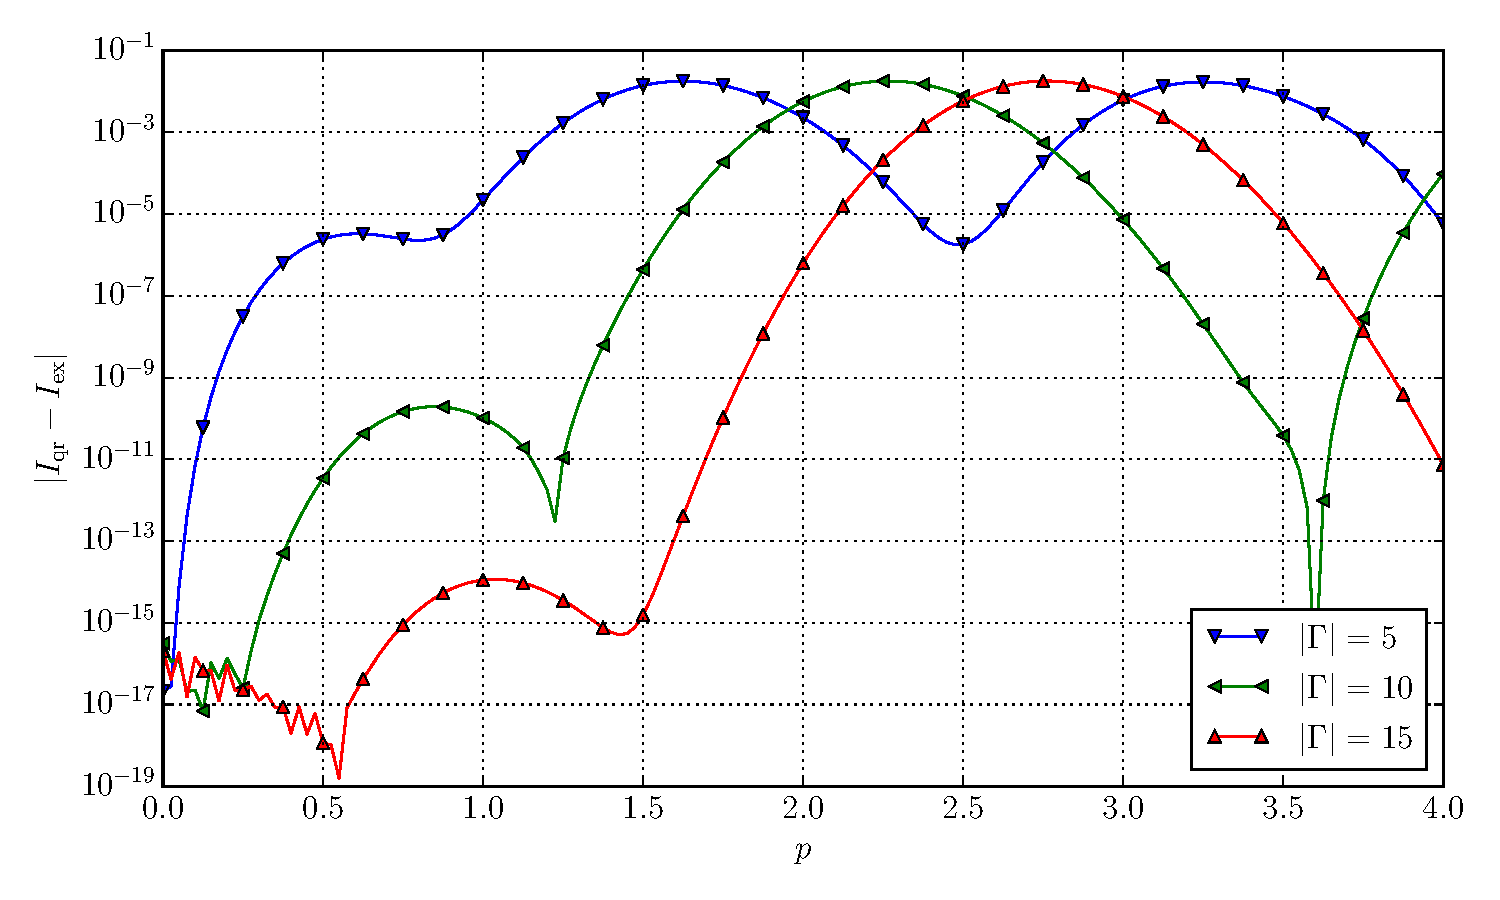
\includegraphics[width=\linewidth]{./plots/tp_4d_conv_p_(0,0,0,0)_(0,0,0,0)_err_qr.pdf}
    \caption{Absolute error of the Gauss-Hermite quadrature compared to the exact solution.}
    \label{fig:tp_4d_conv_p_0000_0000_err_qr}
  \end{subfigure}
  \begin{subfigure}{0.5\linewidth}
    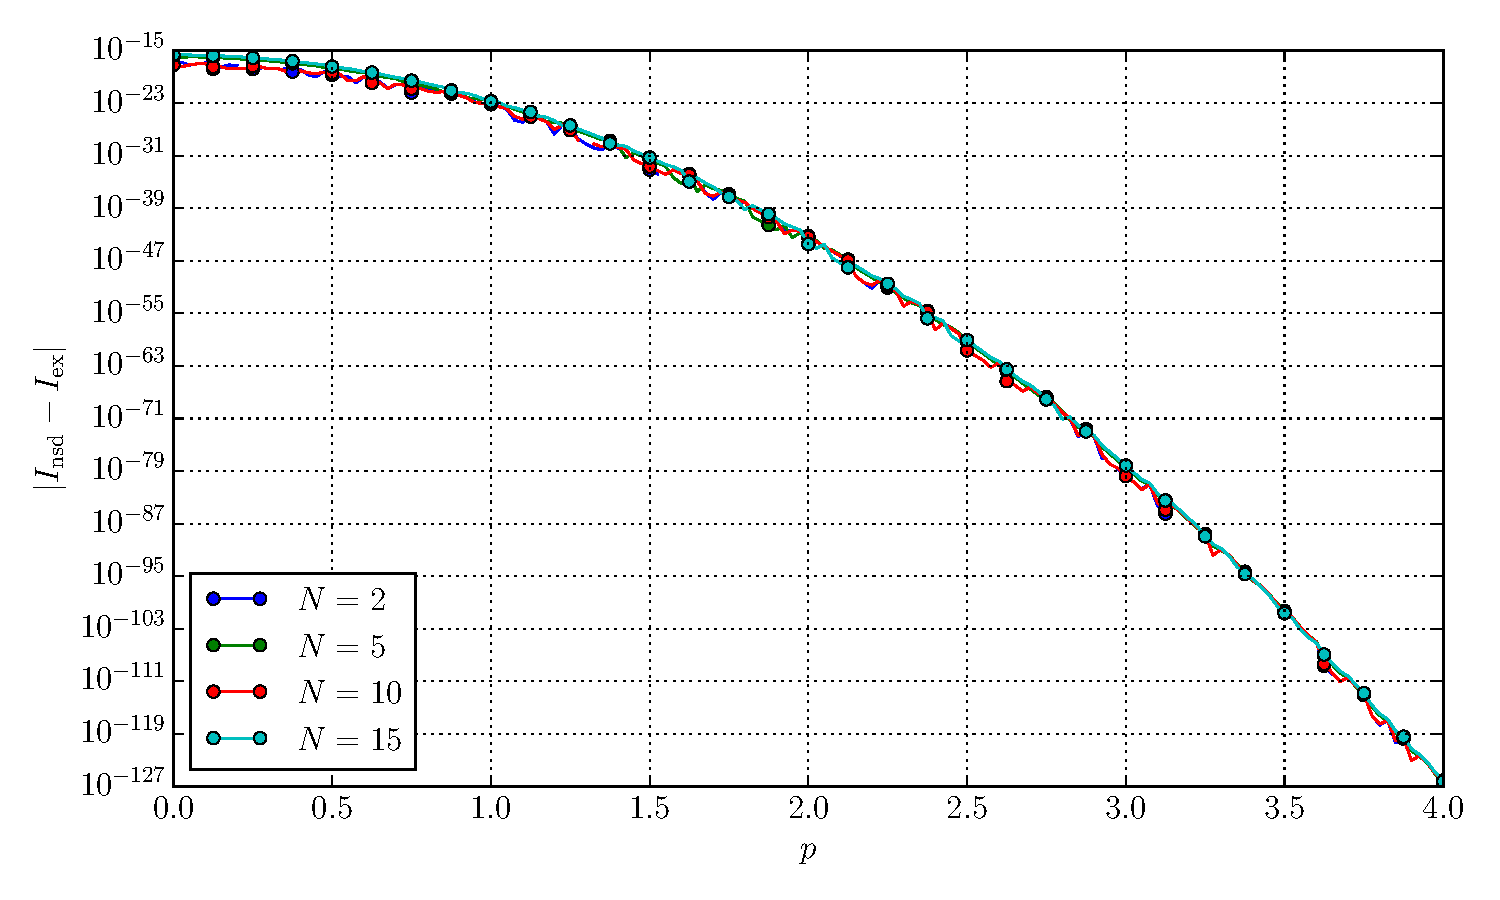
\includegraphics[width=\linewidth]{./plots/tp_4d_conv_p_(0,0,0,0)_(0,0,0,0)_err_nsd.pdf}
    \caption{Absolute error of the steepest descent method compared to the exact solution.}
    \label{fig:tp_4d_conv_p_0000_0000_err_nsd}
  \end{subfigure}
  \begin{subfigure}{0.5\linewidth}
    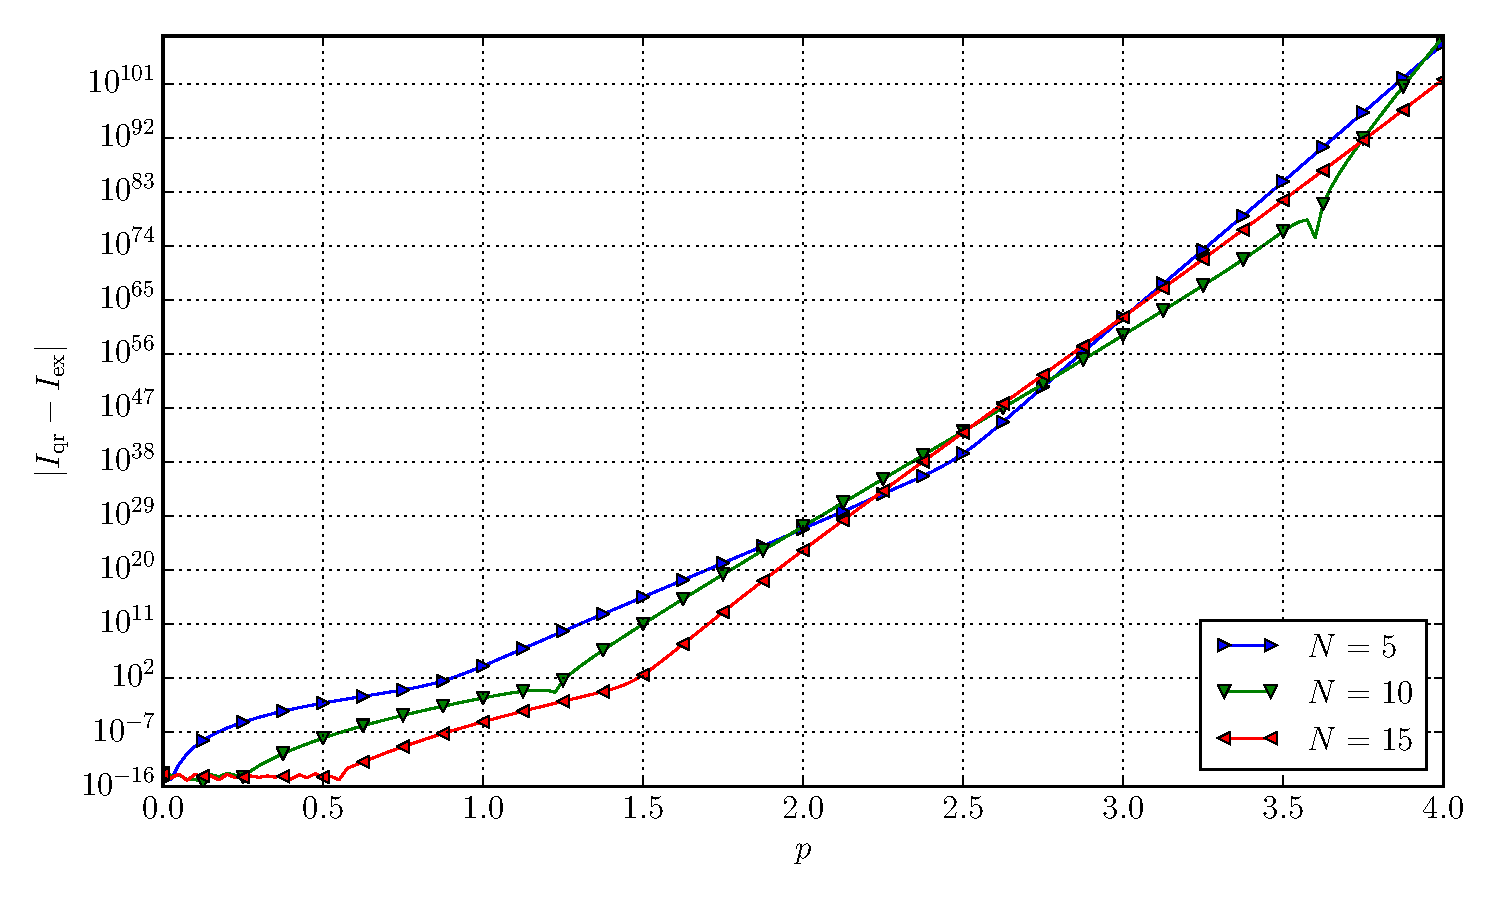
\includegraphics[width=\linewidth]{./plots/tp_4d_conv_p_(0,0,0,0)_(0,0,0,0)_err_rel_qr.pdf}
    \caption{Relative error of the Gauss-Hermite quadrature compared to the exact solution.}
    \label{fig:tp_4d_conv_p_0000_0000_err_qr}
  \end{subfigure}
  \begin{subfigure}{0.5\linewidth}
    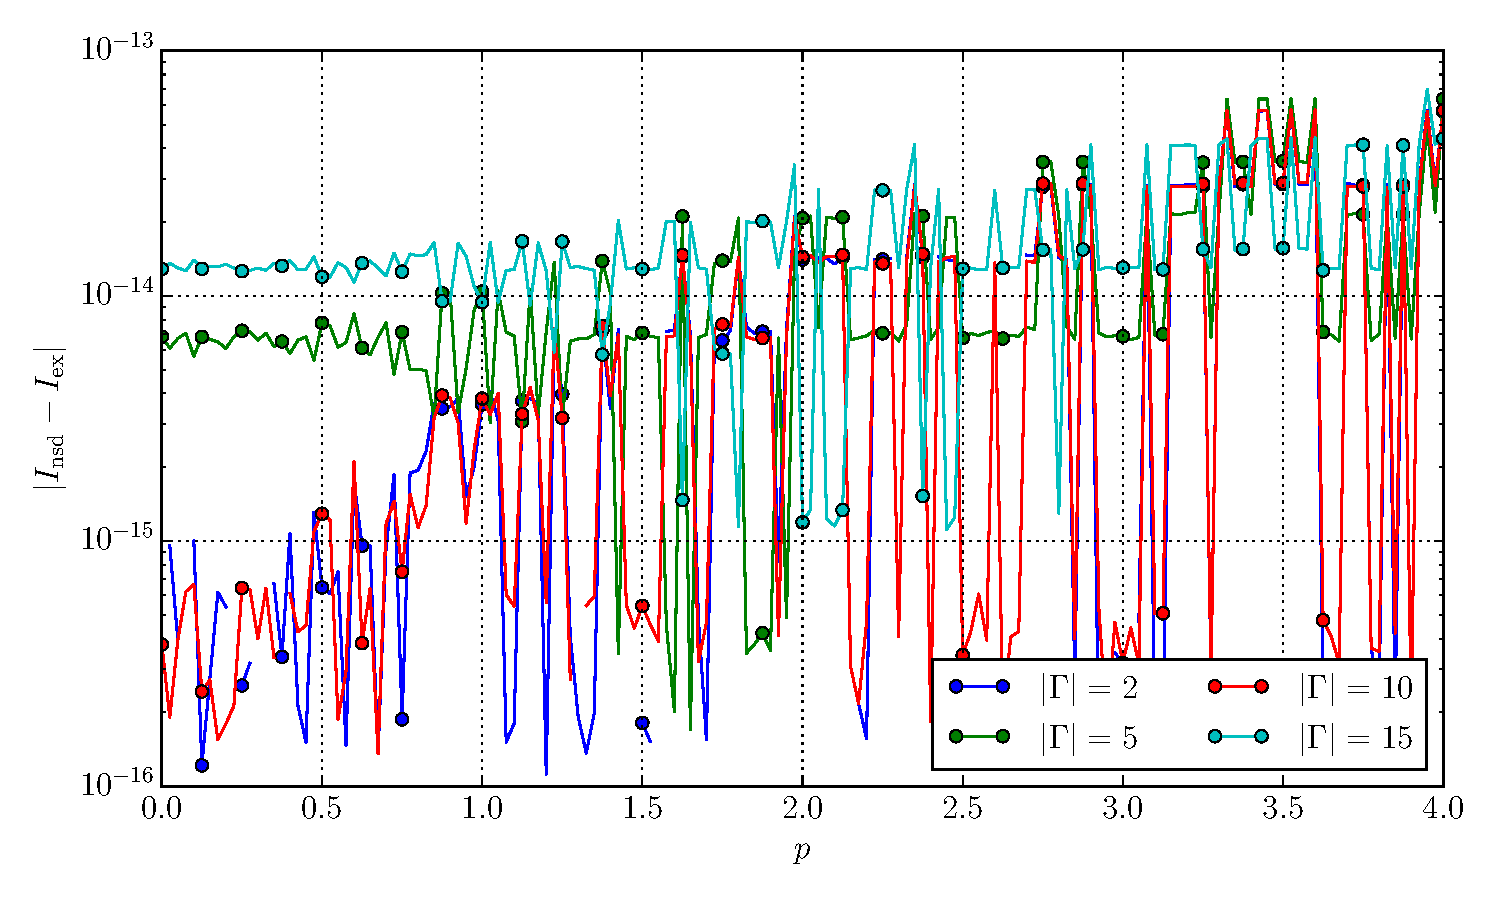
\includegraphics[width=\linewidth]{./plots/tp_4d_conv_p_(0,0,0,0)_(0,0,0,0)_err_rel_nsd.pdf}
    \caption{Relative error of the steepest descent method compared to the exact solution.}
    \label{fig:tp_4d_conv_p_0000_0000_err_nsd}
  \end{subfigure}
  \label{fig:tp_4d_conv_p_0000_0000}
  \caption{Experiment with $\phi_{0,0,0,0}$ and $\phi_{0,0,0,0}^{\prime}$.
  The parameters are:
  $\vec{q} = (-0.1, -0.1, -0.1, -0.1)$,
  $\vec{p} = ( 0.2, -0.2, -0.2,  0.2)$,
  $\mat{Q} = \mat{1}$,
  $\mat{P} = \imath \mat{1}$
  and
  $\vec{q}^\prime = ( 0.1, 0.1, 0.1,  0.1)$,
  $\vec{p}^\prime = (-0.2, 0.2, 0.2, -0.2)$,
  $\mat{Q}^\prime = \mat{1}$,
  $\mat{P}^\prime = \imath \mat{1}$
  with $\varepsilon=0.1$.}
\end{figure}

\begin{figure}
  \begin{subfigure}{0.5\linewidth}
    \includegraphics[width=\linewidth]{./plots/tp_4d_conv_p_(1,1,1,1)_(1,1,1,1)_val_qr.pdf}
    \caption{Gauss-Hermite quadrature with $|\Gamma|$ nodes.}
    \label{fig:tp_4d_conv_p_1111_1111_val_qr}
  \end{subfigure}
  \begin{subfigure}{0.5\linewidth}
    \includegraphics[width=\linewidth]{./plots/tp_4d_conv_p_(1,1,1,1)_(1,1,1,1)_val_nsd.pdf}
    \caption{Steepest descent transformation and quadrature with $|\Gamma|$ nodes.}
    \label{fig:tp_4d_conv_p_1111_1111_val_nsd}
  \end{subfigure} \\
  \begin{subfigure}{0.5\linewidth}
    \includegraphics[width=\linewidth]{./plots/tp_4d_conv_p_(1,1,1,1)_(1,1,1,1)_err_qr.pdf}
    \caption{Absolute error of the Gauss-Hermite quadrature compared to the exact solution.}
    \label{fig:tp_4d_conv_p_1111_1111_err_qr}
  \end{subfigure}
  \begin{subfigure}{0.5\linewidth}
    \includegraphics[width=\linewidth]{./plots/tp_4d_conv_p_(1,1,1,1)_(1,1,1,1)_err_nsd.pdf}
    \caption{Absolute error of the steepest descent method compared to the exact solution.}
    \label{fig:tp_4d_conv_p_1111_1111_err_nsd}
  \end{subfigure}
  \begin{subfigure}{0.5\linewidth}
    \includegraphics[width=\linewidth]{./plots/tp_4d_conv_p_(1,1,1,1)_(1,1,1,1)_err_rel_qr.pdf}
    \caption{Relative error of the Gauss-Hermite quadrature compared to the exact solution.}
    \label{fig:tp_4d_conv_p_1111_1111_err_qr}
  \end{subfigure}
  \begin{subfigure}{0.5\linewidth}
    \includegraphics[width=\linewidth]{./plots/tp_4d_conv_p_(1,1,1,1)_(1,1,1,1)_err_rel_nsd.pdf}
    \caption{Relative error of the steepest descent method compared to the exact solution.}
    \label{fig:tp_4d_conv_p_1111_1111_err_nsd}
  \end{subfigure}
  \label{fig:tp_4d_conv_p_1111_1111}
  \caption{Experiment with $\phi_{1,1,1,1}$ and $\phi_{1,1,1,1}^{\prime}$.
  The parameters are:
  $\vec{q} = (-0.1, -0.1, -0.1, -0.1)$,
  $\vec{p} = ( 0.2, -0.2, -0.2,  0.2)$,
  $\mat{Q} = \mat{1}$,
  $\mat{P} = \imath \mat{1}$
  and
  $\vec{q}^\prime = ( 0.1, 0.1, 0.1,  0.1)$,
  $\vec{p}^\prime = (-0.2, 0.2, 0.2, -0.2)$,
  $\mat{Q}^\prime = \mat{1}$,
  $\mat{P}^\prime = \imath \mat{1}$
  with $\varepsilon=0.1$.}
\end{figure}


\FloatBarrier
\subsubsection{Convergence in $\varepsilon$}


\begin{figure}
  \begin{subfigure}{0.5\linewidth}
    \includegraphics[width=\linewidth]{./plots/tp_1d_conv_eps_0_0_val_qr.pdf}
    \caption{Gauss-Hermite quadrature with $|\Gamma|$ nodes.}
    \label{fig:tp_1d_conv_eps_0_0_val_qr}
  \end{subfigure}
  \begin{subfigure}{0.5\linewidth}
    \includegraphics[width=\linewidth]{./plots/tp_1d_conv_eps_0_0_val_nsd.pdf}
    \caption{Steepest descent transformation and quadrature with $|\Gamma|$ nodes.}
    \label{fig:tp_1d_conv_eps_0_0_val_nsd}
  \end{subfigure} \\
  \begin{subfigure}{0.5\linewidth}
    \includegraphics[width=\linewidth]{./plots/tp_1d_conv_eps_0_0_err_qr.pdf}
    \caption{Absolute error of the Gauss-Hermite quadrature compared to the exact solution.}
    \label{fig:tp_1d_conv_eps_0_0_err_qr}
  \end{subfigure}
  \begin{subfigure}{0.5\linewidth}
    \includegraphics[width=\linewidth]{./plots/tp_1d_conv_eps_0_0_err_nsd.pdf}
    \caption{Absolute error of the steepest descent method compared to the exact solution.}
    \label{fig:tp_1d_conv_eps_0_0_err_nsd}
  \end{subfigure}
  \begin{subfigure}{0.5\linewidth}
    \includegraphics[width=\linewidth]{./plots/tp_1d_conv_eps_0_0_err_rel_qr.pdf}
    \caption{Relative error of the Gauss-Hermite quadrature compared to the exact solution.}
    \label{fig:tp_1d_conv_eps_0_0_err_qr}
  \end{subfigure}
  \begin{subfigure}{0.5\linewidth}
    \includegraphics[width=\linewidth]{./plots/tp_1d_conv_eps_0_0_err_rel_nsd.pdf}
    \caption{Relative error of the steepest descent method compared to the exact solution.}
    \label{fig:tp_1d_conv_eps_0_0_err_nsd}
  \end{subfigure}
  \label{fig:tp_1d_conv_eps_0_0}
  \caption{Experiment with $\phi_{0}$ and $\phi_{0}^{\prime}$.
  The parameters are:
  $q=1.0$, $p=0.2$, $Q=0.5$, $P=2.0\imath$ and
  $q^\prime=1.0$, $p^\prime=-0.2$, $Q^\prime=2.0$, $P^\prime=0.5\imath$.}
\end{figure}

\begin{figure}
  \begin{subfigure}{0.5\linewidth}
    \includegraphics[width=\linewidth]{./plots/tp_1d_conv_eps_2_1_val_qr.pdf}
    \caption{Gauss-Hermite quadrature with $|\Gamma|$ nodes.}
    \label{fig:tp_1d_conv_eps_2_1_val_qr}
  \end{subfigure}
  \begin{subfigure}{0.5\linewidth}
    \includegraphics[width=\linewidth]{./plots/tp_1d_conv_eps_2_1_val_nsd.pdf}
    \caption{Steepest descent transformation and quadrature with $|\Gamma|$ nodes.}
    \label{fig:tp_1d_conv_eps_2_1_val_nsd}
  \end{subfigure} \\
  \begin{subfigure}{0.5\linewidth}
    \includegraphics[width=\linewidth]{./plots/tp_1d_conv_eps_2_1_err_qr.pdf}
    \caption{Absolute error of the Gauss-Hermite quadrature compared to the exact solution.}
    \label{fig:tp_1d_conv_eps_2_1_err_qr}
  \end{subfigure}
  \begin{subfigure}{0.5\linewidth}
    \includegraphics[width=\linewidth]{./plots/tp_1d_conv_eps_2_1_err_nsd.pdf}
    \caption{Absolute error of the steepest descent method compared to the exact solution.}
    \label{fig:tp_1d_conv_eps_2_1_err_nsd}
  \end{subfigure}
  \begin{subfigure}{0.5\linewidth}
    \includegraphics[width=\linewidth]{./plots/tp_1d_conv_eps_2_1_err_rel_qr.pdf}
    \caption{Relative error of the Gauss-Hermite quadrature compared to the exact solution.}
    \label{fig:tp_1d_conv_eps_2_1_err_qr}
  \end{subfigure}
  \begin{subfigure}{0.5\linewidth}
    \includegraphics[width=\linewidth]{./plots/tp_1d_conv_eps_2_1_err_rel_nsd.pdf}
    \caption{Relative error of the steepest descent method compared to the exact solution.}
    \label{fig:tp_1d_conv_eps_2_1_err_nsd}
  \end{subfigure}
  \label{fig:tp_1d_conv_eps_2_1}
  \caption{Experiment with $\phi_{2}$ and $\phi_{1}^{\prime}$.
  The parameters are:
  $q=1.0$, $p=0.2$, $Q=0.5$, $P=2.0\imath$ and
  $q^\prime=1.0$, $p^\prime=-0.2$, $Q^\prime=2.0$, $P^\prime=0.5\imath$.}
\end{figure}

\begin{figure}
  \begin{subfigure}{0.5\linewidth}
    \includegraphics[width=\linewidth]{./plots/tp_1d_conv_eps_8_8_val_qr.pdf}
    \caption{Gauss-Hermite quadrature with $|\Gamma|$ nodes.}
    \label{fig:tp_1d_conv_eps_8_8_val_qr}
  \end{subfigure}
  \begin{subfigure}{0.5\linewidth}
    \includegraphics[width=\linewidth]{./plots/tp_1d_conv_eps_8_8_val_nsd.pdf}
    \caption{Steepest descent transformation and quadrature with $|\Gamma|$ nodes.}
    \label{fig:tp_1d_conv_eps_8_8_val_nsd}
  \end{subfigure} \\
  \begin{subfigure}{0.5\linewidth}
    \includegraphics[width=\linewidth]{./plots/tp_1d_conv_eps_8_8_err_qr.pdf}
    \caption{Absolute error of the Gauss-Hermite quadrature compared to the exact solution.}
    \label{fig:tp_1d_conv_eps_8_8_err_qr}
  \end{subfigure}
  \begin{subfigure}{0.5\linewidth}
    \includegraphics[width=\linewidth]{./plots/tp_1d_conv_eps_8_8_err_nsd.pdf}
    \caption{Absolute error of the steepest descent method compared to the exact solution.}
    \label{fig:tp_1d_conv_eps_8_8_err_nsd}
  \end{subfigure}
  \begin{subfigure}{0.5\linewidth}
    \includegraphics[width=\linewidth]{./plots/tp_1d_conv_eps_8_8_err_rel_qr.pdf}
    \caption{Relative error of the Gauss-Hermite quadrature compared to the exact solution.}
    \label{fig:tp_1d_conv_eps_8_8_err_qr}
  \end{subfigure}
  \begin{subfigure}{0.5\linewidth}
    \includegraphics[width=\linewidth]{./plots/tp_1d_conv_eps_8_8_err_rel_nsd.pdf}
    \caption{Relative error of the steepest descent method compared to the exact solution.}
    \label{fig:tp_1d_conv_eps_8_8_err_nsd}
  \end{subfigure}
  \label{fig:tp_1d_conv_eps_8_8}
  \caption{Experiment with $\phi_{8}$ and $\phi_{8}^{\prime}$.
  The parameters are:
  $q=1.0$, $p=0.2$, $Q=0.5$, $P=2.0\imath$ and
  $q^\prime=1.0$, $p^\prime=-0.2$, $Q^\prime=2.0$, $P^\prime=0.5\imath$.}
\end{figure}

\begin{figure}
  \begin{subfigure}{0.5\linewidth}
    \includegraphics[width=\linewidth]{./plots/tp_2d_conv_eps_(0,0)_(0,0)_val_qr.pdf}
    \caption{Gauss-Hermite quadrature with $|\Gamma|$ nodes.}
    \label{fig:tp_2d_conv_eps_00_00_val_qr}
  \end{subfigure}
  \begin{subfigure}{0.5\linewidth}
    \includegraphics[width=\linewidth]{./plots/tp_2d_conv_eps_(0,0)_(0,0)_val_nsd.pdf}
    \caption{Steepest descent transformation and quadrature with $|\Gamma|$ nodes.}
    \label{fig:tp_2d_conv_eps_00_00_val_nsd}
  \end{subfigure} \\
  \begin{subfigure}{0.5\linewidth}
    \includegraphics[width=\linewidth]{./plots/tp_2d_conv_eps_(0,0)_(0,0)_err_qr.pdf}
    \caption{Absolute error of the Gauss-Hermite quadrature compared to the exact solution.}
    \label{fig:tp_2d_conv_eps_00_00_err_qr}
  \end{subfigure}
  \begin{subfigure}{0.5\linewidth}
    \includegraphics[width=\linewidth]{./plots/tp_2d_conv_eps_(0,0)_(0,0)_err_nsd.pdf}
    \caption{Absolute error of the steepest descent method compared to the exact solution.}
    \label{fig:tp_2d_conv_eps_00_00_err_nsd}
  \end{subfigure}
  \begin{subfigure}{0.5\linewidth}
    \includegraphics[width=\linewidth]{./plots/tp_2d_conv_eps_(0,0)_(0,0)_err_rel_qr.pdf}
    \caption{Relative error of the Gauss-Hermite quadrature compared to the exact solution.}
    \label{fig:tp_2d_conv_eps_00_00_err_qr}
  \end{subfigure}
  \begin{subfigure}{0.5\linewidth}
    \includegraphics[width=\linewidth]{./plots/tp_2d_conv_eps_(0,0)_(0,0)_err_rel_nsd.pdf}
    \caption{Relative error of the steepest descent method compared to the exact solution.}
    \label{fig:tp_2d_conv_eps_00_00_err_nsd}
  \end{subfigure}
  \label{fig:tp_2d_conv_eps_00_00}
  \caption{Experiment with $\phi_{0,0}$ and $\phi_{0,0}^{\prime}$.
  The parameters are:
  $\vec{q} = (1, 1)$,
  $\vec{p} = (-0.2, -0.2)$,
  $\mat{Q} = \mat{1}$,
  $\mat{P} = \imath \mat{1}$
  and
  $\vec{q}^\prime = (1, 1)$,
  $\vec{p}^\prime = (0.2, 0.2)$,
  $\mat{Q}^\prime = \mat{1}$,
  $\mat{P}^\prime = \imath \mat{1}$.}
\end{figure}

\begin{figure}
  \begin{subfigure}{0.5\linewidth}
    \includegraphics[width=\linewidth]{./plots/tp_2d_conv_eps_(0,1)_(1,0)_val_qr.pdf}
    \caption{Gauss-Hermite quadrature with $|\Gamma|$ nodes.}
    \label{fig:tp_2d_conv_eps_01_10_val_qr}
  \end{subfigure}
  \begin{subfigure}{0.5\linewidth}
    \includegraphics[width=\linewidth]{./plots/tp_2d_conv_eps_(0,1)_(1,0)_val_nsd.pdf}
    \caption{Steepest descent transformation and quadrature with $|\Gamma|$ nodes.}
    \label{fig:tp_2d_conv_eps_01_10_val_nsd}
  \end{subfigure} \\
  \begin{subfigure}{0.5\linewidth}
    \includegraphics[width=\linewidth]{./plots/tp_2d_conv_eps_(0,1)_(1,0)_err_qr.pdf}
    \caption{Absolute error of the Gauss-Hermite quadrature compared to the exact solution.}
    \label{fig:tp_2d_conv_eps_01_10_err_qr}
  \end{subfigure}
  \begin{subfigure}{0.5\linewidth}
    \includegraphics[width=\linewidth]{./plots/tp_2d_conv_eps_(0,1)_(1,0)_err_nsd.pdf}
    \caption{Absolute error of the steepest descent method compared to the exact solution.}
    \label{fig:tp_2d_conv_eps_01_10_err_nsd}
  \end{subfigure}
  \begin{subfigure}{0.5\linewidth}
    \includegraphics[width=\linewidth]{./plots/tp_2d_conv_eps_(0,1)_(1,0)_err_rel_qr.pdf}
    \caption{Relative error of the Gauss-Hermite quadrature compared to the exact solution.}
    \label{fig:tp_2d_conv_eps_01_10_err_qr}
  \end{subfigure}
  \begin{subfigure}{0.5\linewidth}
    \includegraphics[width=\linewidth]{./plots/tp_2d_conv_eps_(0,1)_(1,0)_err_rel_nsd.pdf}
    \caption{Relative error of the steepest descent method compared to the exact solution.}
    \label{fig:tp_2d_conv_eps_01_10_err_nsd}
  \end{subfigure}
  \label{fig:tp_2d_conv_eps_01_10}
  \caption{Experiment with $\phi_{0,1}$ and $\phi_{1,0}^{\prime}$.
  The parameters are:
  $\vec{q} = (1, 1)$,
  $\vec{p} = (-0.2, -0.2)$,
  $\mat{Q} = \mat{1}$,
  $\mat{P} = \imath \mat{1}$
  and
  $\vec{q}^\prime = (1, 1)$,
  $\vec{p}^\prime = (0.2, 0.2)$,
  $\mat{Q}^\prime = \mat{1}$,
  $\mat{P}^\prime = \imath \mat{1}$.}
\end{figure}

\begin{figure}
  \begin{subfigure}{0.5\linewidth}
    \includegraphics[width=\linewidth]{./plots/tp_2d_conv_eps_(2,3)_(2,2)_val_qr.pdf}
    \caption{Gauss-Hermite quadrature with $|\Gamma|$ nodes.}
    \label{fig:tp_2d_conv_eps_23_22_val_qr}
  \end{subfigure}
  \begin{subfigure}{0.5\linewidth}
    \includegraphics[width=\linewidth]{./plots/tp_2d_conv_eps_(2,3)_(2,2)_val_nsd.pdf}
    \caption{Steepest descent transformation and quadrature with $|\Gamma|$ nodes.}
    \label{fig:tp_2d_conv_eps_23_22_val_nsd}
  \end{subfigure} \\
  \begin{subfigure}{0.5\linewidth}
    \includegraphics[width=\linewidth]{./plots/tp_2d_conv_eps_(2,3)_(2,2)_err_qr.pdf}
    \caption{Absolute error of the Gauss-Hermite quadrature compared to the exact solution.}
    \label{fig:tp_2d_conv_eps_23_22_err_qr}
  \end{subfigure}
  \begin{subfigure}{0.5\linewidth}
    \includegraphics[width=\linewidth]{./plots/tp_2d_conv_eps_(2,3)_(2,2)_err_nsd.pdf}
    \caption{Absolute error of the steepest descent method compared to the exact solution.}
    \label{fig:tp_2d_conv_eps_23_22_err_nsd}
  \end{subfigure}
  \begin{subfigure}{0.5\linewidth}
    \includegraphics[width=\linewidth]{./plots/tp_2d_conv_eps_(2,3)_(2,2)_err_rel_qr.pdf}
    \caption{Relative error of the Gauss-Hermite quadrature compared to the exact solution.}
    \label{fig:tp_2d_conv_eps_23_22_err_qr}
  \end{subfigure}
  \begin{subfigure}{0.5\linewidth}
    \includegraphics[width=\linewidth]{./plots/tp_2d_conv_eps_(2,3)_(2,2)_err_rel_nsd.pdf}
    \caption{Relative error of the steepest descent method compared to the exact solution.}
    \label{fig:tp_2d_conv_eps_23_22_err_nsd}
  \end{subfigure}
  \label{fig:tp_2d_conv_eps_23_22}
  \caption{Experiment with $\phi_{2,3}$ and $\phi_{2,2}^{\prime}$.
  The parameters are:
  $\vec{q} = (1, 1)$,
  $\vec{p} = (-0.2, -0.2)$,
  $\mat{Q} = \mat{1}$,
  $\mat{P} = \imath \mat{1}$
  and
  $\vec{q}^\prime = (1, 1)$,
  $\vec{p}^\prime = (0.2, 0.2)$,
  $\mat{Q}^\prime = \mat{1}$,
  $\mat{P}^\prime = \imath \mat{1}$.}
\end{figure}

\begin{figure}
  \begin{subfigure}{0.5\linewidth}
    \includegraphics[width=\linewidth]{./plots/tp_4d_conv_eps_(0,0,0,0)_(0,0,0,0)_val_qr.pdf}
    \caption{Gauss-Hermite quadrature with $|\Gamma|$ nodes.}
    \label{fig:tp_4d_conv_eps_0000_0000_val_qr}
  \end{subfigure}
  \begin{subfigure}{0.5\linewidth}
    \includegraphics[width=\linewidth]{./plots/tp_4d_conv_eps_(0,0,0,0)_(0,0,0,0)_val_nsd.pdf}
    \caption{Steepest descent transformation and quadrature with $|\Gamma|$ nodes.}
    \label{fig:tp_4d_conv_eps_0000_0000_val_nsd}
  \end{subfigure} \\
  \begin{subfigure}{0.5\linewidth}
    \includegraphics[width=\linewidth]{./plots/tp_4d_conv_eps_(0,0,0,0)_(0,0,0,0)_err_qr.pdf}
    \caption{Absolute error of the Gauss-Hermite quadrature compared to the exact solution.}
    \label{fig:tp_4d_conv_eps_0000_0000_err_qr}
  \end{subfigure}
  \begin{subfigure}{0.5\linewidth}
    \includegraphics[width=\linewidth]{./plots/tp_4d_conv_eps_(0,0,0,0)_(0,0,0,0)_err_nsd.pdf}
    \caption{Absolute error of the steepest descent method compared to the exact solution.}
    \label{fig:tp_4d_conv_eps_0000_0000_err_nsd}
  \end{subfigure}
  \begin{subfigure}{0.5\linewidth}
    \includegraphics[width=\linewidth]{./plots/tp_4d_conv_eps_(0,0,0,0)_(0,0,0,0)_err_rel_qr.pdf}
    \caption{Relative error of the Gauss-Hermite quadrature compared to the exact solution.}
    \label{fig:tp_4d_conv_eps_0000_0000_err_qr}
  \end{subfigure}
  \begin{subfigure}{0.5\linewidth}
    \includegraphics[width=\linewidth]{./plots/tp_4d_conv_eps_(0,0,0,0)_(0,0,0,0)_err_rel_nsd.pdf}
    \caption{Relative error of the steepest descent method compared to the exact solution.}
    \label{fig:tp_4d_conv_eps_0000_0000_err_nsd}
  \end{subfigure}
  \label{fig:tp_4d_conv_eps_0000_0000}
  \caption{Experiment with $\phi_{0,0,0,0}$ and $\phi_{0,0,0,0}^{\prime}$.
  The parameters are:
  $\vec{q} = (1, 1, 1, 1)$,
  $\vec{p} = (-0.5, -0.5, -0.5, -0.5)$,
  $\mat{Q} = \mat{1}$,
  $\mat{P} = \imath \mat{1}$
  and
  $\vec{q}^\prime = (1, 1, 1, 1)$,
  $\vec{p}^\prime = (0.5, 0.5, 0.5, 0.5)$,
  $\mat{Q}^\prime = \mat{1}$,
  $\mat{P}^\prime = \imath \mat{1}$.}
\end{figure}

\begin{figure}
  \begin{subfigure}{0.5\linewidth}
    \includegraphics[width=\linewidth]{./plots/tp_4d_conv_eps_(2,1,2,1)_(1,1,1,1)_val_qr.pdf}
    \caption{Gauss-Hermite quadrature with $|\Gamma|$ nodes.}
    \label{fig:tp_4d_conv_eps_2121_1111_val_qr}
  \end{subfigure}
  \begin{subfigure}{0.5\linewidth}
    \includegraphics[width=\linewidth]{./plots/tp_4d_conv_eps_(2,1,2,1)_(1,1,1,1)_val_nsd.pdf}
    \caption{Steepest descent transformation and quadrature with $|\Gamma|$ nodes.}
    \label{fig:tp_4d_conv_eps_2121_1111_val_nsd}
  \end{subfigure} \\
  \begin{subfigure}{0.5\linewidth}
    \includegraphics[width=\linewidth]{./plots/tp_4d_conv_eps_(2,1,2,1)_(1,1,1,1)_err_qr.pdf}
    \caption{Absolute error of the Gauss-Hermite quadrature compared to the exact solution.}
    \label{fig:tp_4d_conv_eps_2121_1111_err_qr}
  \end{subfigure}
  \begin{subfigure}{0.5\linewidth}
    \includegraphics[width=\linewidth]{./plots/tp_4d_conv_eps_(2,1,2,1)_(1,1,1,1)_err_nsd.pdf}
    \caption{Absolute error of the steepest descent method compared to the exact solution.}
    \label{fig:tp_4d_conv_eps_2121_1111_err_nsd}
  \end{subfigure}
  \begin{subfigure}{0.5\linewidth}
    \includegraphics[width=\linewidth]{./plots/tp_4d_conv_eps_(2,1,2,1)_(1,1,1,1)_err_rel_qr.pdf}
    \caption{Relative error of the Gauss-Hermite quadrature compared to the exact solution.}
    \label{fig:tp_4d_conv_eps_2121_1111_err_qr}
  \end{subfigure}
  \begin{subfigure}{0.5\linewidth}
    \includegraphics[width=\linewidth]{./plots/tp_4d_conv_eps_(2,1,2,1)_(1,1,1,1)_err_rel_nsd.pdf}
    \caption{Relative error of the steepest descent method compared to the exact solution.}
    \label{fig:tp_4d_conv_eps_2121_1111_err_nsd}
  \end{subfigure}
  \label{fig:tp_4d_conv_eps_2121_1111}
  \caption{Experiment with $\phi_{2,1,2,1}$ and $\phi_{1,1,1,1}^{\prime}$.
  The parameters are:
  $\vec{q} = (1, 1, 1, 1)$,
  $\vec{p} = (-0.5, -0.5, -0.5, -0.5)$,
  $\mat{Q} = \mat{1}$,
  $\mat{P} = \imath \mat{1}$
  and
  $\vec{q}^\prime = (1, 1, 1, 1)$,
  $\vec{p}^\prime = (0.5, 0.5, 0.5, 0.5)$,
  $\mat{Q}^\prime = \mat{1}$,
  $\mat{P}^\prime = \imath \mat{1}$.}
\end{figure}


Show that we need still $N^D$ quadrature nodes
but that $N$ is much smaller than for traditional
schemes.


\FloatBarrier
\subsubsection{Higher dimensions}


\begin{figure}
  \begin{subfigure}{0.5\linewidth}
    \includegraphics[width=\linewidth]{./plots/tp_sg_3d_conv_p_(0,0,0)_(0,0,0)_val_nsd_tp.pdf}
    \caption{Tensor product of linear size $N$ with a total of $|\Gamma|$ quadrature nodes.}
    \label{fig:tp_sg_3d_conv_p_000_000_val_nsd_tp}
  \end{subfigure}
  \begin{subfigure}{0.5\linewidth}
    \includegraphics[width=\linewidth]{./plots/tp_sg_3d_conv_p_(0,0,0)_(0,0,0)_val_nsd_gk.pdf}
    \caption{Smolyak construction of level $K$ with a total of $|\Gamma|$ quadrature nodes.}
    \label{fig:tp_sg_3d_conv_p_000_000_val_nsd_gk.pdf}
  \end{subfigure} \\
  \begin{subfigure}{0.5\linewidth}
    \includegraphics[width=\linewidth]{./plots/tp_sg_3d_conv_p_(0,0,0)_(0,0,0)_err_nsd_tp.pdf}
    \caption{Absolute error of the tensor product ansatz compared to the exact solution.}
    \label{fig:tp_sg_3d_conv_p_000_000_err_nsd_tp}
  \end{subfigure}
  \begin{subfigure}{0.5\linewidth}
    \includegraphics[width=\linewidth]{./plots/tp_sg_3d_conv_p_(0,0,0)_(0,0,0)_err_nsd_gk.pdf}
    \caption{Absolute error of the Smolyak construction compared to the exact solution.}
    \label{fig:tp_sg_3d_conv_p_000_000_err_nsd_gk}
  \end{subfigure}
  \begin{subfigure}{0.5\linewidth}
    \includegraphics[width=\linewidth]{./plots/tp_sg_3d_conv_p_(0,0,0)_(0,0,0)_err_rel_nsd_tp.pdf}
    \caption{Relative error of the tensor product ansatz compared to the exact solution.}
    \label{fig:tp_sg_3d_conv_p_000_000_err_rel_nsd_tp}
  \end{subfigure}
  \begin{subfigure}{0.5\linewidth}
    \includegraphics[width=\linewidth]{./plots/tp_sg_3d_conv_p_(0,0,0)_(0,0,0)_err_rel_nsd_gk.pdf}
    \caption{Relative error of the Smolyak construction compared to the exact solution.}
    \label{fig:tp_sg_3d_conv_p_000_000_err_rel_nsd_gk}
  \end{subfigure}
  \label{fig:tp_sg_3d_conv_p_000_000}
  \caption{Experiment with $\phi_{0,0,0}$ and $\phi_{0,0,0}^{\prime}$
  in 3 dimensions.
  The parameters are:
  $\vec{q} = (1.2,1.2,1.2)$,
  $\vec{p} = (1,1,1)$,
  $\mat{Q} = \mat{1}$,
  $\mat{P} = \imath \mat{1}$
  and
  $\vec{q}^\prime = (0.8,0.8,0.8)$,
  $\vec{p}^\prime = (-1,-1,-1)$,
  $\mat{Q}^\prime = \mat{1}$,
  $\mat{P}^\prime = \imath \mat{1}$
  with $\varepsilon=0.3$.}
\end{figure}

\begin{figure}
  \begin{subfigure}{0.5\linewidth}
    \includegraphics[width=\linewidth]{./plots/tp_sg_3d_conv_p_(0,1,1)_(1,1,0)_val_nsd_tp.pdf}
    \caption{Tensor product of linear size $N$ with a total of $|\Gamma|$ quadrature nodes.}
    \label{fig:tp_sg_3d_conv_p_011_110_val_nsd_tp}
  \end{subfigure}
  \begin{subfigure}{0.5\linewidth}
    \includegraphics[width=\linewidth]{./plots/tp_sg_3d_conv_p_(0,1,1)_(1,1,0)_val_nsd_gk.pdf}
    \caption{Smolyak construction of level $K$ with a total of $|\Gamma|$ quadrature nodes.}
    \label{fig:tp_sg_3d_conv_p_011_110_val_nsd_gk.pdf}
  \end{subfigure} \\
  \begin{subfigure}{0.5\linewidth}
    \includegraphics[width=\linewidth]{./plots/tp_sg_3d_conv_p_(0,1,1)_(1,1,0)_err_nsd_tp.pdf}
    \caption{Absolute error of the tensor product ansatz compared to the exact solution.}
    \label{fig:tp_sg_3d_conv_p_011_110_err_nsd_tp}
  \end{subfigure}
  \begin{subfigure}{0.5\linewidth}
    \includegraphics[width=\linewidth]{./plots/tp_sg_3d_conv_p_(0,1,1)_(1,1,0)_err_nsd_gk.pdf}
    \caption{Absolute error of the Smolyak construction compared to the exact solution.}
    \label{fig:tp_sg_3d_conv_p_011_110_err_nsd_gk}
  \end{subfigure}
  \begin{subfigure}{0.5\linewidth}
    \includegraphics[width=\linewidth]{./plots/tp_sg_3d_conv_p_(0,1,1)_(1,1,0)_err_rel_nsd_tp.pdf}
    \caption{Relative error of the tensor product ansatz compared to the exact solution.}
    \label{fig:tp_sg_3d_conv_p_011_110_err_rel_nsd_tp}
  \end{subfigure}
  \begin{subfigure}{0.5\linewidth}
    \includegraphics[width=\linewidth]{./plots/tp_sg_3d_conv_p_(0,1,1)_(1,1,0)_err_rel_nsd_gk.pdf}
    \caption{Relative error of the Smolyak construction compared to the exact solution.}
    \label{fig:tp_sg_3d_conv_p_011_110_err_rel_nsd_gk}
  \end{subfigure}
  \label{fig:tp_sg_3d_conv_p_011_110}
  \caption{Experiment with $\phi_{0,1,1}$ and $\phi_{1,1,0}^{\prime}$
  in 3 dimensions.
  The parameters are:
  $\vec{q} = 1.2 (1,\ldots,1)$,
  $\vec{p} = (1,\ldots,1)$,
  $\mat{Q} = \mat{1}$,
  $\mat{P} = \imath \mat{1}$
  and
  $\vec{q}^\prime = 0.8 (1,\ldots,1)$,
  $\vec{p}^\prime = -(1,\ldots,1)$,
  $\mat{Q}^\prime = \mat{1}$,
  $\mat{P}^\prime = \imath \mat{1}$
  with $\varepsilon=0.3$.}
\end{figure}

\begin{figure}
  \begin{subfigure}{0.5\linewidth}
    \includegraphics[width=\linewidth]{./plots/tp_sg_3d_conv_p_(0,4,0)_(4,0,0)_val_nsd_tp.pdf}
    \caption{Tensor product of linear size $N$ with a total of $|\Gamma|$ quadrature nodes.}
    \label{fig:tp_sg_3d_conv_p_040_400_val_nsd_tp}
  \end{subfigure}
  \begin{subfigure}{0.5\linewidth}
    \includegraphics[width=\linewidth]{./plots/tp_sg_3d_conv_p_(0,4,0)_(4,0,0)_val_nsd_gk.pdf}
    \caption{Smolyak construction of level $K$ with a total of $|\Gamma|$ quadrature nodes.}
    \label{fig:tp_sg_3d_conv_p_040_400_val_nsd_gk.pdf}
  \end{subfigure} \\
  \begin{subfigure}{0.5\linewidth}
    \includegraphics[width=\linewidth]{./plots/tp_sg_3d_conv_p_(0,4,0)_(4,0,0)_err_nsd_tp.pdf}
    \caption{Absolute error of the tensor product ansatz compared to the exact solution.}
    \label{fig:tp_sg_3d_conv_p_040_400_err_nsd_tp}
  \end{subfigure}
  \begin{subfigure}{0.5\linewidth}
    \includegraphics[width=\linewidth]{./plots/tp_sg_3d_conv_p_(0,4,0)_(4,0,0)_err_nsd_gk.pdf}
    \caption{Absolute error of the Smolyak construction compared to the exact solution.}
    \label{fig:tp_sg_3d_conv_p_040_400_err_nsd_gk}
  \end{subfigure}
  \begin{subfigure}{0.5\linewidth}
    \includegraphics[width=\linewidth]{./plots/tp_sg_3d_conv_p_(0,4,0)_(4,0,0)_err_rel_nsd_tp.pdf}
    \caption{Relative error of the tensor product ansatz compared to the exact solution.}
    \label{fig:tp_sg_3d_conv_p_040_400_err_rel_nsd_tp}
  \end{subfigure}
  \begin{subfigure}{0.5\linewidth}
    \includegraphics[width=\linewidth]{./plots/tp_sg_3d_conv_p_(0,4,0)_(4,0,0)_err_rel_nsd_gk.pdf}
    \caption{Relative error of the Smolyak construction compared to the exact solution.}
    \label{fig:tp_sg_3d_conv_p_040_400_err_rel_nsd_gk}
  \end{subfigure}
  \label{fig:tp_sg_3d_conv_p_040_400}
  \caption{Experiment with $\phi_{0,4,0}$ and $\phi_{4,0,0}^{\prime}$
  in 3 dimensions.
  The parameters are:
  $\vec{q} = 1.2 (1,\ldots,1)$,
  $\vec{p} = (1,\ldots,1)$,
  $\mat{Q} = \mat{1}$,
  $\mat{P} = \imath \mat{1}$
  and
  $\vec{q}^\prime = 0.8 (1,\ldots,1)$,
  $\vec{p}^\prime = -(1,\ldots,1)$,
  $\mat{Q}^\prime = \mat{1}$,
  $\mat{P}^\prime = \imath \mat{1}$
  with $\varepsilon=0.3$.}
\end{figure}

\begin{figure}
  \begin{subfigure}{0.5\linewidth}
    \includegraphics[width=\linewidth]{./plots/tp_sg_3d_conv_p_(4,4,4)_(4,4,4)_val_nsd_tp.pdf}
    \caption{Tensor product of linear size $N$ with a total of $|\Gamma|$ quadrature nodes.}
    \label{fig:tp_sg_3d_conv_p_444_444_val_nsd_tp}
  \end{subfigure}
  \begin{subfigure}{0.5\linewidth}
    \includegraphics[width=\linewidth]{./plots/tp_sg_3d_conv_p_(4,4,4)_(4,4,4)_val_nsd_gk.pdf}
    \caption{Smolyak construction of level $K$ with a total of $|\Gamma|$ quadrature nodes.}
    \label{fig:tp_sg_3d_conv_p_444_444_val_nsd_gk.pdf}
  \end{subfigure} \\
  \begin{subfigure}{0.5\linewidth}
    \includegraphics[width=\linewidth]{./plots/tp_sg_3d_conv_p_(4,4,4)_(4,4,4)_err_nsd_tp.pdf}
    \caption{Absolute error of the tensor product ansatz compared to the exact solution.}
    \label{fig:tp_sg_3d_conv_p_444_444_err_nsd_tp}
  \end{subfigure}
  \begin{subfigure}{0.5\linewidth}
    \includegraphics[width=\linewidth]{./plots/tp_sg_3d_conv_p_(4,4,4)_(4,4,4)_err_nsd_gk.pdf}
    \caption{Absolute error of the Smolyak construction compared to the exact solution.}
    \label{fig:tp_sg_3d_conv_p_444_444_err_nsd_gk}
  \end{subfigure}
  \begin{subfigure}{0.5\linewidth}
    \includegraphics[width=\linewidth]{./plots/tp_sg_3d_conv_p_(4,4,4)_(4,4,4)_err_rel_nsd_tp.pdf}
    \caption{Relative error of the tensor product ansatz compared to the exact solution.}
    \label{fig:tp_sg_3d_conv_p_444_444_err_rel_nsd_tp}
  \end{subfigure}
  \begin{subfigure}{0.5\linewidth}
    \includegraphics[width=\linewidth]{./plots/tp_sg_3d_conv_p_(4,4,4)_(4,4,4)_err_rel_nsd_gk.pdf}
    \caption{Relative error of the Smolyak construction compared to the exact solution.}
    \label{fig:tp_sg_3d_conv_p_444_444_err_rel_nsd_gk}
  \end{subfigure}
  \label{fig:tp_sg_3d_conv_p_444_444}
  \caption{Experiment with $\phi_{4,4,4}$ and $\phi_{4,4,4}^{\prime}$
  in 3 dimensions.
  The parameters are:
  $\vec{q} = 1.2 (1,\ldots,1)$,
  $\vec{p} = (1,\ldots,1)$,
  $\mat{Q} = \mat{1}$,
  $\mat{P} = \imath \mat{1}$
  and
  $\vec{q}^\prime = 0.8 (1,\ldots,1)$,
  $\vec{p}^\prime = -(1,\ldots,1)$,
  $\mat{Q}^\prime = \mat{1}$,
  $\mat{P}^\prime = \imath \mat{1}$
  with $\varepsilon=0.3$.}
\end{figure}

\begin{figure}
  \begin{subfigure}{0.5\linewidth}
    \includegraphics[width=\linewidth]{./plots/tp_sg_4d_conv_p_(0,2,1,1)_(1,2,1,0)_val_nsd_tp.pdf}
    \caption{Tensor product of linear size $N$ with a total of $|\Gamma|$ quadrature nodes.}
    \label{fig:tp_sg_4d_conv_p_(0,2,1,1)_(1,2,1,0)_val_nsd_tp}
  \end{subfigure}
  \begin{subfigure}{0.5\linewidth}
    \includegraphics[width=\linewidth]{./plots/tp_sg_4d_conv_p_(0,2,1,1)_(1,2,1,0)_val_nsd_gk.pdf}
    \caption{Smolyak construction of level $K$ with a total of $|\Gamma|$ quadrature nodes.}
    \label{fig:tp_sg_4d_conv_p_(0,2,1,1)_(1,2,1,0)_val_nsd_gk.pdf}
  \end{subfigure} \\
  \begin{subfigure}{0.5\linewidth}
    \includegraphics[width=\linewidth]{./plots/tp_sg_4d_conv_p_(0,2,1,1)_(1,2,1,0)_err_nsd_tp.pdf}
    \caption{Absolute error of the tensor product ansatz compared to the exact solution.}
    \label{fig:tp_sg_4d_conv_p_(0,2,1,1)_(1,2,1,0)_err_nsd_tp}
  \end{subfigure}
  \begin{subfigure}{0.5\linewidth}
    \includegraphics[width=\linewidth]{./plots/tp_sg_4d_conv_p_(0,2,1,1)_(1,2,1,0)_err_nsd_gk.pdf}
    \caption{Absolute error of the Smolyak construction compared to the exact solution.}
    \label{fig:tp_sg_4d_conv_p_(0,2,1,1)_(1,2,1,0)_err_nsd_gk}
  \end{subfigure}
  \begin{subfigure}{0.5\linewidth}
    \includegraphics[width=\linewidth]{./plots/tp_sg_4d_conv_p_(0,2,1,1)_(1,2,1,0)_err_rel_nsd_tp.pdf}
    \caption{Relative error of the tensor product ansatz compared to the exact solution.}
    \label{fig:tp_sg_4d_conv_p_(0,2,1,1)_(1,2,1,0)_err_rel_nsd_tp}
  \end{subfigure}
  \begin{subfigure}{0.5\linewidth}
    \includegraphics[width=\linewidth]{./plots/tp_sg_4d_conv_p_(0,2,1,1)_(1,2,1,0)_err_rel_nsd_gk.pdf}
    \caption{Relative error of the Smolyak construction compared to the exact solution.}
    \label{fig:tp_sg_4d_conv_p_(0,2,1,1)_(1,2,1,0)_err_rel_nsd_gk}
  \end{subfigure}
  \label{fig:tp_sg_4d_conv_p_0211_1210}
  \caption{Experiment with $\phi_{0,2,1,1}$ and $\phi_{1,2,1,0}^{\prime}$
  in 4 dimensions.
  The parameters are:
  $\vec{q} = 1.01 (1,\ldots,1)$,
  $\vec{p} = (1,\ldots,1)$,
  $\mat{Q} = \mat{1}$,
  $\mat{P} = \imath \mat{1}$
  and
  $\vec{q}^\prime = 0.99 (1,\ldots,1)$,
  $\vec{p}^\prime = -(1,\ldots,1)$,
  $\mat{Q}^\prime = \mat{1}$,
  $\mat{P}^\prime = \imath \mat{1}$
  with $\varepsilon=0.3$.}
\end{figure}

\begin{figure}
  \begin{subfigure}{0.5\linewidth}
    \includegraphics[width=\linewidth]{./plots/tp_sg_6d_conv_p_(0,0,0,0,0,0)_(0,0,0,0,0,0)_val_nsd_tp.pdf}
    \caption{Tensor product of linear size $N$ with a total of $|\Gamma|$ quadrature nodes.}
    \label{fig:tp_sg_6d_conv_p_(0,0,0,0,0,0)_(0,0,0,0,0,0)_val_nsd_tp}
  \end{subfigure}
  \begin{subfigure}{0.5\linewidth}
    \includegraphics[width=\linewidth]{./plots/tp_sg_6d_conv_p_(0,0,0,0,0,0)_(0,0,0,0,0,0)_val_nsd_gk.pdf}
    \caption{Smolyak construction of level $K$ with a total of $|\Gamma|$ quadrature nodes.}
    \label{fig:tp_sg_6d_conv_p_(0,0,0,0,0,0)_(0,0,0,0,0,0)_val_nsd_gk.pdf}
  \end{subfigure} \\
  \begin{subfigure}{0.5\linewidth}
    \includegraphics[width=\linewidth]{./plots/tp_sg_6d_conv_p_(0,0,0,0,0,0)_(0,0,0,0,0,0)_err_nsd_tp.pdf}
    \caption{Absolute error of the tensor product ansatz compared to the exact solution.}
    \label{fig:tp_sg_6d_conv_p_(0,0,0,0,0,0)_(0,0,0,0,0,0)_err_nsd_tp}
  \end{subfigure}
  \begin{subfigure}{0.5\linewidth}
    \includegraphics[width=\linewidth]{./plots/tp_sg_6d_conv_p_(0,0,0,0,0,0)_(0,0,0,0,0,0)_err_nsd_gk.pdf}
    \caption{Absolute error of the Smolyak construction compared to the exact solution.}
    \label{fig:tp_sg_6d_conv_p_(0,0,0,0,0,0)_(0,0,0,0,0,0)_err_nsd_gk}
  \end{subfigure}
  \begin{subfigure}{0.5\linewidth}
    \includegraphics[width=\linewidth]{./plots/tp_sg_6d_conv_p_(0,0,0,0,0,0)_(0,0,0,0,0,0)_err_rel_nsd_tp.pdf}
    \caption{Relative error of the tensor product ansatz compared to the exact solution.}
    \label{fig:tp_sg_6d_conv_p_(0,0,0,0,0,0)_(0,0,0,0,0,0)_err_rel_nsd_tp}
  \end{subfigure}
  \begin{subfigure}{0.5\linewidth}
    \includegraphics[width=\linewidth]{./plots/tp_sg_6d_conv_p_(0,0,0,0,0,0)_(0,0,0,0,0,0)_err_rel_nsd_gk.pdf}
    \caption{Relative error of the Smolyak construction compared to the exact solution.}
    \label{fig:tp_sg_6d_conv_p_(0,0,0,0,0,0)_(0,0,0,0,0,0)_err_rel_nsd_gk}
  \end{subfigure}
  \label{fig:tp_sg_6d_conv_p_000000_000000}
  \caption{Experiment with $\phi_{\vec{0}}$ and $\phi_{\vec{0}}^{\prime}$
  in 6 dimensions.
  The parameters are:
  $\vec{q} = 1.01 (1,\ldots,1)$,
  $\vec{p} = (1,\ldots,1)$,
  $\mat{Q} = \mat{1}$,
  $\mat{P} = \imath \mat{1}$
  and
  $\vec{q}^\prime = 0.99 (1,\ldots,1)$,
  $\vec{p}^\prime = -(1,\ldots,1)$,
  $\mat{Q}^\prime = \mat{1}$,
  $\mat{P}^\prime = \imath \mat{1}$
  with $\varepsilon=0.3$.}
\end{figure}

\begin{figure}
  \begin{subfigure}{0.5\linewidth}
    \includegraphics[width=\linewidth]{./plots/tp_sg_6d_conv_p_(1,0,1,0,0,0)_(1,1,0,0,0,0)_val_nsd_tp.pdf}
    \caption{Tensor product of linear size $N$ with a total of $|\Gamma|$ quadrature nodes.}
    \label{fig:tp_sg_6d_conv_p_(1,0,1,0,0,0)_(1,1,0,0,0,0)_val_nsd_tp}
  \end{subfigure}
  \begin{subfigure}{0.5\linewidth}
    \includegraphics[width=\linewidth]{./plots/tp_sg_6d_conv_p_(1,0,1,0,0,0)_(1,1,0,0,0,0)_val_nsd_gk.pdf}
    \caption{Smolyak construction of level $K$ with a total of $|\Gamma|$ quadrature nodes.}
    \label{fig:tp_sg_6d_conv_p_(1,0,1,0,0,0)_(1,1,0,0,0,0)_val_nsd_gk.pdf}
  \end{subfigure} \\
  \begin{subfigure}{0.5\linewidth}
    \includegraphics[width=\linewidth]{./plots/tp_sg_6d_conv_p_(1,0,1,0,0,0)_(1,1,0,0,0,0)_err_nsd_tp.pdf}
    \caption{Absolute error of the tensor product ansatz compared to the exact solution.}
    \label{fig:tp_sg_6d_conv_p_(1,0,1,0,0,0)_(1,1,0,0,0,0)_err_nsd_tp}
  \end{subfigure}
  \begin{subfigure}{0.5\linewidth}
    \includegraphics[width=\linewidth]{./plots/tp_sg_6d_conv_p_(1,0,1,0,0,0)_(1,1,0,0,0,0)_err_nsd_gk.pdf}
    \caption{Absolute error of the Smolyak construction compared to the exact solution.}
    \label{fig:tp_sg_6d_conv_p_(1,0,1,0,0,0)_(1,1,0,0,0,0)_err_nsd_gk}
  \end{subfigure}
  \begin{subfigure}{0.5\linewidth}
    \includegraphics[width=\linewidth]{./plots/tp_sg_6d_conv_p_(1,0,1,0,0,0)_(1,1,0,0,0,0)_err_rel_nsd_tp.pdf}
    \caption{Relative error of the tensor product ansatz compared to the exact solution.}
    \label{fig:tp_sg_6d_conv_p_(1,0,1,0,0,0)_(1,1,0,0,0,0)_err_rel_nsd_tp}
  \end{subfigure}
  \begin{subfigure}{0.5\linewidth}
    \includegraphics[width=\linewidth]{./plots/tp_sg_6d_conv_p_(1,0,1,0,0,0)_(1,1,0,0,0,0)_err_rel_nsd_gk.pdf}
    \caption{Relative error of the Smolyak construction compared to the exact solution.}
    \label{fig:tp_sg_6d_conv_p_(1,0,1,0,0,0)_(1,1,0,0,0,0)_err_rel_nsd_gk}
  \end{subfigure}
  \label{fig:tp_sg_6d_conv_p_101000_110000}
  \caption{Experiment with $\phi_{1,0,1,0,0,0}$ and $\phi_{1,1,0,0,0,0}^{\prime}$
  in 6 dimensions.
  The parameters are:
  $\vec{q} = 1.01 (1,\ldots,1)$,
  $\vec{p} = (1,\ldots,1)$,
  $\mat{Q} = \mat{1}$,
  $\mat{P} = \imath \mat{1}$
  and
  $\vec{q}^\prime = 0.99 (1,\ldots,1)$,
  $\vec{p}^\prime = -(1,\ldots,1)$,
  $\mat{Q}^\prime = \mat{1}$,
  $\mat{P}^\prime = \imath \mat{1}$
  with $\varepsilon=0.3$.}
\end{figure}

\begin{figure}
  \begin{subfigure}{0.5\linewidth}
    \includegraphics[width=\linewidth]{./plots/tp_sg_12d_conv_p_(0,0,0,0,0,0,0,0,0,0,0,0)_(0,0,0,0,0,0,0,0,0,0,0,0)_val_nsd_tp.pdf}
    \caption{Tensor product of linear size $N$ with a total of $|\Gamma|$ quadrature nodes.}
    \label{fig:tp_sg_12d_conv_p_(0,0,0,0,0,0,0,0,0,0,0,0)_(0,0,0,0,0,0,0,0,0,0,0,0)_val_nsd_tp}
  \end{subfigure}
  \begin{subfigure}{0.5\linewidth}
    \includegraphics[width=\linewidth]{./plots/tp_sg_12d_conv_p_(0,0,0,0,0,0,0,0,0,0,0,0)_(0,0,0,0,0,0,0,0,0,0,0,0)_val_nsd_gk.pdf}
    \caption{Smolyak construction of level $K$ with a total of $|\Gamma|$ quadrature nodes.}
    \label{fig:tp_sg_12d_conv_p_(0,0,0,0,0,0,0,0,0,0,0,0)_(0,0,0,0,0,0,0,0,0,0,0,0)_val_nsd_gk.pdf}
  \end{subfigure} \\
  \begin{subfigure}{0.5\linewidth}
    \includegraphics[width=\linewidth]{./plots/tp_sg_12d_conv_p_(0,0,0,0,0,0,0,0,0,0,0,0)_(0,0,0,0,0,0,0,0,0,0,0,0)_err_nsd_tp.pdf}
    \caption{Absolute error of the tensor product ansatz compared to the exact solution.}
    \label{fig:tp_sg_12d_conv_p_(0,0,0,0,0,0,0,0,0,0,0,0)_(0,0,0,0,0,0,0,0,0,0,0,0)_err_nsd_tp}
  \end{subfigure}
  \begin{subfigure}{0.5\linewidth}
    \includegraphics[width=\linewidth]{./plots/tp_sg_12d_conv_p_(0,0,0,0,0,0,0,0,0,0,0,0)_(0,0,0,0,0,0,0,0,0,0,0,0)_err_nsd_gk.pdf}
    \caption{Absolute error of the Smolyak construction compared to the exact solution.}
    \label{fig:tp_sg_12d_conv_p_(0,0,0,0,0,0,0,0,0,0,0,0)_(0,0,0,0,0,0,0,0,0,0,0,0)_err_nsd_gk}
  \end{subfigure}
  \begin{subfigure}{0.5\linewidth}
    \includegraphics[width=\linewidth]{./plots/tp_sg_12d_conv_p_(0,0,0,0,0,0,0,0,0,0,0,0)_(0,0,0,0,0,0,0,0,0,0,0,0)_err_rel_nsd_tp.pdf}
    \caption{Relative error of the tensor product ansatz compared to the exact solution.}
    \label{fig:tp_sg_12d_conv_p_(0,0,0,0,0,0,0,0,0,0,0,0)_(0,0,0,0,0,0,0,0,0,0,0,0)_err_rel_nsd_tp}
  \end{subfigure}
  \begin{subfigure}{0.5\linewidth}
    \includegraphics[width=\linewidth]{./plots/tp_sg_12d_conv_p_(0,0,0,0,0,0,0,0,0,0,0,0)_(0,0,0,0,0,0,0,0,0,0,0,0)_err_rel_nsd_gk.pdf}
    \caption{Relative error of the Smolyak construction compared to the exact solution.}
    \label{fig:tp_sg_12d_conv_p_(0,0,0,0,0,0,0,0,0,0,0,0)_(0,0,0,0,0,0,0,0,0,0,0,0)_err_rel_nsd_gk}
  \end{subfigure}
  \label{fig:tp_sg_12d_conv_p_000000000000_000000000000}
  \caption{Experiment with $\phi_{\vec{0}}$ and $\phi_{\vec{0}}^{\prime}$
  in 12 dimensions.
  The parameters are:
  $\vec{q} = 1.0001 (1,\ldots,1)$,
  $\vec{p} = (1,\ldots,1)$,
  $\mat{Q} = \mat{1}$,
  $\mat{P} = \imath \mat{1}$
  and
  $\vec{q}^\prime = 0.9999 (1,\ldots,1)$,
  $\vec{p}^\prime = -(1,\ldots,1)$,
  $\mat{Q}^\prime = \mat{1}$,
  $\mat{P}^\prime = \imath \mat{1}$
  with $\varepsilon=0.3$.}
\end{figure}


\FloatBarrier
\subsubsection{Convergence in $\varepsilon$}


\begin{figure}
  \begin{subfigure}{0.5\linewidth}
    \includegraphics[width=\linewidth]{./plots/tp_sg_3d_conv_eps_(0,0,0)_(0,0,0)_val_nsd_tp.pdf}
    \caption{Tensor product of linear size $N$ with a total of $|\Gamma|$ quadrature nodes.}
    \label{fig:tp_sg_3d_conv_p_000_000_val_nsd_tp}
  \end{subfigure}
  \begin{subfigure}{0.5\linewidth}
    \includegraphics[width=\linewidth]{./plots/tp_sg_3d_conv_eps_(0,0,0)_(0,0,0)_val_nsd_gk.pdf}
    \caption{Smolyak construction of level $K$ with a total of $|\Gamma|$ quadrature nodes.}
    \label{fig:tp_sg_3d_conv_p_000_000_val_nsd_gk.pdf}
  \end{subfigure} \\
  \begin{subfigure}{0.5\linewidth}
    \includegraphics[width=\linewidth]{./plots/tp_sg_3d_conv_eps_(0,0,0)_(0,0,0)_err_nsd_tp.pdf}
    \caption{Absolute error of the tensor product ansatz compared to the exact solution.}
    \label{fig:tp_sg_3d_conv_p_000_000_err_nsd_tp}
  \end{subfigure}
  \begin{subfigure}{0.5\linewidth}
    \includegraphics[width=\linewidth]{./plots/tp_sg_3d_conv_eps_(0,0,0)_(0,0,0)_err_nsd_gk.pdf}
    \caption{Absolute error of the Smolyak construction compared to the exact solution.}
    \label{fig:tp_sg_3d_conv_p_000_000_err_nsd_gk}
  \end{subfigure}
  \begin{subfigure}{0.5\linewidth}
    \includegraphics[width=\linewidth]{./plots/tp_sg_3d_conv_eps_(0,0,0)_(0,0,0)_err_rel_nsd_tp.pdf}
    \caption{Relative error of the tensor product ansatz compared to the exact solution.}
    \label{fig:tp_sg_3d_conv_p_000_000_err_rel_nsd_tp}
  \end{subfigure}
  \begin{subfigure}{0.5\linewidth}
    \includegraphics[width=\linewidth]{./plots/tp_sg_3d_conv_eps_(0,0,0)_(0,0,0)_err_rel_nsd_gk.pdf}
    \caption{Relative error of the Smolyak construction compared to the exact solution.}
    \label{fig:tp_sg_3d_conv_p_000_000_err_rel_nsd_gk}
  \end{subfigure}
  \label{fig:tp_sg_3d_conv_p_000_000}
  \caption{Experiment with $\phi_{0,0,0}$ and $\phi_{0,0,0}^{\prime}$
  in 3 dimensions.
  The parameters are:
  $\vec{q} = (1, 1, 1)$,
  $\vec{p} = (-0.2, -0.2, -0.2)$,
  $\mat{Q} = \mat{1}$,
  $\mat{P} = \imath \mat{1}$
  and
  $\vec{q}^\prime = (1, 1, 1)$,
  $\vec{p}^\prime = (0.2, 0.2, 0.2)$,
  $\mat{Q}^\prime = \mat{1}$,
  $\mat{P}^\prime = \imath \mat{1}$.}
\end{figure}

\begin{figure}
  \begin{subfigure}{0.5\linewidth}
    \includegraphics[width=\linewidth]{./plots/tp_sg_3d_conv_eps_(1,1,0)_(0,1,1)_val_nsd_tp.pdf}
    \caption{Tensor product of linear size $N$ with a total of $|\Gamma|$ quadrature nodes.}
    \label{fig:tp_sg_3d_conv_p_110_011_val_nsd_tp}
  \end{subfigure}
  \begin{subfigure}{0.5\linewidth}
    \includegraphics[width=\linewidth]{./plots/tp_sg_3d_conv_eps_(1,1,0)_(0,1,1)_val_nsd_gk.pdf}
    \caption{Smolyak construction of level $K$ with a total of $|\Gamma|$ quadrature nodes.}
    \label{fig:tp_sg_3d_conv_p_110_011_val_nsd_gk.pdf}
  \end{subfigure} \\
  \begin{subfigure}{0.5\linewidth}
    \includegraphics[width=\linewidth]{./plots/tp_sg_3d_conv_eps_(1,1,0)_(0,1,1)_err_nsd_tp.pdf}
    \caption{Absolute error of the tensor product ansatz compared to the exact solution.}
    \label{fig:tp_sg_3d_conv_p_110_011_err_nsd_tp}
  \end{subfigure}
  \begin{subfigure}{0.5\linewidth}
    \includegraphics[width=\linewidth]{./plots/tp_sg_3d_conv_eps_(1,1,0)_(0,1,1)_err_nsd_gk.pdf}
    \caption{Absolute error of the Smolyak construction compared to the exact solution.}
    \label{fig:tp_sg_3d_conv_p_110_011_err_nsd_gk}
  \end{subfigure}
  \begin{subfigure}{0.5\linewidth}
    \includegraphics[width=\linewidth]{./plots/tp_sg_3d_conv_eps_(1,1,0)_(0,1,1)_err_rel_nsd_tp.pdf}
    \caption{Relative error of the tensor product ansatz compared to the exact solution.}
    \label{fig:tp_sg_3d_conv_p_110_011_err_rel_nsd_tp}
  \end{subfigure}
  \begin{subfigure}{0.5\linewidth}
    \includegraphics[width=\linewidth]{./plots/tp_sg_3d_conv_eps_(1,1,0)_(0,1,1)_err_rel_nsd_gk.pdf}
    \caption{Relative error of the Smolyak construction compared to the exact solution.}
    \label{fig:tp_sg_3d_conv_p_110_011_err_rel_nsd_gk}
  \end{subfigure}
  \label{fig:tp_sg_3d_conv_p_110_011}
  \caption{Experiment with $\phi_{1,1,0}$ and $\phi_{0,1,1}^{\prime}$
  in 3 dimensions.
  The parameters are:
  $\vec{q} = (1, 1, 1)$,
  $\vec{p} = (-0.2, -0.2, -0.2)$,
  $\mat{Q} = \mat{1}$,
  $\mat{P} = \imath \mat{1}$
  and
  $\vec{q}^\prime = (1, 1, 1)$,
  $\vec{p}^\prime = (0.2, 0.2, 0.2)$,
  $\mat{Q}^\prime = \mat{1}$,
  $\mat{P}^\prime = \imath \mat{1}$.}
\end{figure}

\begin{figure}
  \begin{subfigure}{0.5\linewidth}
    \includegraphics[width=\linewidth]{./plots/tp_sg_3d_conv_eps_(4,0,0)_(0,4,0)_val_nsd_tp.pdf}
    \caption{Tensor product of linear size $N$ with a total of $|\Gamma|$ quadrature nodes.}
    \label{fig:tp_sg_3d_conv_p_400_040_val_nsd_tp}
  \end{subfigure}
  \begin{subfigure}{0.5\linewidth}
    \includegraphics[width=\linewidth]{./plots/tp_sg_3d_conv_eps_(4,0,0)_(0,4,0)_val_nsd_gk.pdf}
    \caption{Smolyak construction of level $K$ with a total of $|\Gamma|$ quadrature nodes.}
    \label{fig:tp_sg_3d_conv_p_400_040_val_nsd_gk.pdf}
  \end{subfigure} \\
  \begin{subfigure}{0.5\linewidth}
    \includegraphics[width=\linewidth]{./plots/tp_sg_3d_conv_eps_(4,0,0)_(0,4,0)_err_nsd_tp.pdf}
    \caption{Absolute error of the tensor product ansatz compared to the exact solution.}
    \label{fig:tp_sg_3d_conv_p_400_040_err_nsd_tp}
  \end{subfigure}
  \begin{subfigure}{0.5\linewidth}
    \includegraphics[width=\linewidth]{./plots/tp_sg_3d_conv_eps_(4,0,0)_(0,4,0)_err_nsd_gk.pdf}
    \caption{Absolute error of the Smolyak construction compared to the exact solution.}
    \label{fig:tp_sg_3d_conv_p_400_040_err_nsd_gk}
  \end{subfigure}
  \begin{subfigure}{0.5\linewidth}
    \includegraphics[width=\linewidth]{./plots/tp_sg_3d_conv_eps_(4,0,0)_(0,4,0)_err_rel_nsd_tp.pdf}
    \caption{Relative error of the tensor product ansatz compared to the exact solution.}
    \label{fig:tp_sg_3d_conv_p_400_040_err_rel_nsd_tp}
  \end{subfigure}
  \begin{subfigure}{0.5\linewidth}
    \includegraphics[width=\linewidth]{./plots/tp_sg_3d_conv_eps_(4,0,0)_(0,4,0)_err_rel_nsd_gk.pdf}
    \caption{Relative error of the Smolyak construction compared to the exact solution.}
    \label{fig:tp_sg_3d_conv_p_400_040_err_rel_nsd_gk}
  \end{subfigure}
  \label{fig:tp_sg_3d_conv_p_400_040}
  \caption{Experiment with $\phi_{4,0,0}$ and $\phi_{0,4,0}^{\prime}$
  in 3 dimensions.
  The parameters are:
  $\vec{q} = (1, 1, 1)$,
  $\vec{p} = (-0.2, -0.2, -0.2)$,
  $\mat{Q} = \mat{1}$,
  $\mat{P} = \imath \mat{1}$
  and
  $\vec{q}^\prime = (1, 1, 1)$,
  $\vec{p}^\prime = (0.2, 0.2, 0.2)$,
  $\mat{Q}^\prime = \mat{1}$,
  $\mat{P}^\prime = \imath \mat{1}$.}
\end{figure}

\begin{figure}
  \begin{subfigure}{0.5\linewidth}
    \includegraphics[width=\linewidth]{./plots/tp_sg_3d_conv_eps_(2,2,2)_(2,2,2)_val_nsd_tp.pdf}
    \caption{Tensor product of linear size $N$ with a total of $|\Gamma|$ quadrature nodes.}
    \label{fig:tp_sg_3d_conv_p_222_222_val_nsd_tp}
  \end{subfigure}
  \begin{subfigure}{0.5\linewidth}
    \includegraphics[width=\linewidth]{./plots/tp_sg_3d_conv_eps_(2,2,2)_(2,2,2)_val_nsd_gk.pdf}
    \caption{Smolyak construction of level $K$ with a total of $|\Gamma|$ quadrature nodes.}
    \label{fig:tp_sg_3d_conv_p_222_222_val_nsd_gk.pdf}
  \end{subfigure} \\
  \begin{subfigure}{0.5\linewidth}
    \includegraphics[width=\linewidth]{./plots/tp_sg_3d_conv_eps_(2,2,2)_(2,2,2)_err_nsd_tp.pdf}
    \caption{Absolute error of the tensor product ansatz compared to the exact solution.}
    \label{fig:tp_sg_3d_conv_p_222_222_err_nsd_tp}
  \end{subfigure}
  \begin{subfigure}{0.5\linewidth}
    \includegraphics[width=\linewidth]{./plots/tp_sg_3d_conv_eps_(2,2,2)_(2,2,2)_err_nsd_gk.pdf}
    \caption{Absolute error of the Smolyak construction compared to the exact solution.}
    \label{fig:tp_sg_3d_conv_p_222_222_err_nsd_gk}
  \end{subfigure}
  \begin{subfigure}{0.5\linewidth}
    \includegraphics[width=\linewidth]{./plots/tp_sg_3d_conv_eps_(2,2,2)_(2,2,2)_err_rel_nsd_tp.pdf}
    \caption{Relative error of the tensor product ansatz compared to the exact solution.}
    \label{fig:tp_sg_3d_conv_p_222_222_err_rel_nsd_tp}
  \end{subfigure}
  \begin{subfigure}{0.5\linewidth}
    \includegraphics[width=\linewidth]{./plots/tp_sg_3d_conv_eps_(2,2,2)_(2,2,2)_err_rel_nsd_gk.pdf}
    \caption{Relative error of the Smolyak construction compared to the exact solution.}
    \label{fig:tp_sg_3d_conv_p_222_222_err_rel_nsd_gk}
  \end{subfigure}
  \label{fig:tp_sg_3d_conv_p_222_222}
  \caption{Experiment with $\phi_{2,2,2}$ and $\phi_{2,2,2}^{\prime}$
  in 3 dimensions.
  The parameters are:
  $\vec{q} = (1, 1, 1)$,
  $\vec{p} = (-0.2, -0.2, -0.2)$,
  $\mat{Q} = \mat{1}$,
  $\mat{P} = \imath \mat{1}$
  and
  $\vec{q}^\prime = (1, 1, 1)$,
  $\vec{p}^\prime = (0.2, 0.2, 0.2)$,
  $\mat{Q}^\prime = \mat{1}$,
  $\mat{P}^\prime = \imath \mat{1}$.}
\end{figure}

\begin{figure}
  \begin{subfigure}{0.5\linewidth}
    \includegraphics[width=\linewidth]{./plots/tp_sg_4d_conv_eps_(3,0,0,0)_(3,0,0,0)_val_nsd_tp.pdf}
    \caption{Tensor product of linear size $N$ with a total of $|\Gamma|$ quadrature nodes.}
    \label{fig:tp_sg_4d_conv_p_3000_3000_val_nsd_tp}
  \end{subfigure}
  \begin{subfigure}{0.5\linewidth}
    \includegraphics[width=\linewidth]{./plots/tp_sg_4d_conv_eps_(3,0,0,0)_(3,0,0,0)_val_nsd_gk.pdf}
    \caption{Smolyak construction of level $K$ with a total of $|\Gamma|$ quadrature nodes.}
    \label{fig:tp_sg_4d_conv_p_3000_3000_val_nsd_gk.pdf}
  \end{subfigure} \\
  \begin{subfigure}{0.5\linewidth}
    \includegraphics[width=\linewidth]{./plots/tp_sg_4d_conv_eps_(3,0,0,0)_(3,0,0,0)_err_nsd_tp.pdf}
    \caption{Absolute error of the tensor product ansatz compared to the exact solution.}
    \label{fig:tp_sg_4d_conv_p_3000_3000_err_nsd_tp}
  \end{subfigure}
  \begin{subfigure}{0.5\linewidth}
    \includegraphics[width=\linewidth]{./plots/tp_sg_4d_conv_eps_(3,0,0,0)_(3,0,0,0)_err_nsd_gk.pdf}
    \caption{Absolute error of the Smolyak construction compared to the exact solution.}
    \label{fig:tp_sg_4d_conv_p_3000_3000_err_nsd_gk}
  \end{subfigure}
  \begin{subfigure}{0.5\linewidth}
    \includegraphics[width=\linewidth]{./plots/tp_sg_4d_conv_eps_(3,0,0,0)_(3,0,0,0)_err_rel_nsd_tp.pdf}
    \caption{Relative error of the tensor product ansatz compared to the exact solution.}
    \label{fig:tp_sg_4d_conv_p_3000_3000_err_rel_nsd_tp}
  \end{subfigure}
  \begin{subfigure}{0.5\linewidth}
    \includegraphics[width=\linewidth]{./plots/tp_sg_4d_conv_eps_(3,0,0,0)_(3,0,0,0)_err_rel_nsd_gk.pdf}
    \caption{Relative error of the Smolyak construction compared to the exact solution.}
    \label{fig:tp_sg_4d_conv_p_3000_3000_err_rel_nsd_gk}
  \end{subfigure}
  \label{fig:tp_sg_4d_conv_p_3000_3000}
  \caption{Experiment with $\phi_{3,0,0,0}$ and $\phi_{3,0,0,0}^{\prime}$
  in 4 dimensions.
  The parameters are:
  $\vec{q} = (1, 1, 1, 1)$,
  $\vec{p} = (-0.2, -0.2, -0.2, -0.2)$,
  $\mat{Q} = \mat{1}$,
  $\mat{P} = \imath \mat{1}$
  and
  $\vec{q}^\prime = (1, 1, 1, 1)$,
  $\vec{p}^\prime = (0.2, 0.2, 0.2, 0.2)$,
  $\mat{Q}^\prime = \mat{1}$,
  $\mat{P}^\prime = \imath \mat{1}$.}
\end{figure}

\begin{figure}
  \begin{subfigure}{0.5\linewidth}
    \includegraphics[width=\linewidth]{./plots/tp_sg_4d_conv_eps_(8,0,1,0)_(8,1,0,0)_val_nsd_tp.pdf}
    \caption{Tensor product of linear size $N$ with a total of $|\Gamma|$ quadrature nodes.}
    \label{fig:tp_sg_4d_conv_p_8010_8100_val_nsd_tp}
  \end{subfigure}
  \begin{subfigure}{0.5\linewidth}
    \includegraphics[width=\linewidth]{./plots/tp_sg_4d_conv_eps_(8,0,1,0)_(8,1,0,0)_val_nsd_gk.pdf}
    \caption{Smolyak construction of level $K$ with a total of $|\Gamma|$ quadrature nodes.}
    \label{fig:tp_sg_4d_conv_p_8010_8100_val_nsd_gk.pdf}
  \end{subfigure} \\
  \begin{subfigure}{0.5\linewidth}
    \includegraphics[width=\linewidth]{./plots/tp_sg_4d_conv_eps_(8,0,1,0)_(8,1,0,0)_err_nsd_tp.pdf}
    \caption{Absolute error of the tensor product ansatz compared to the exact solution.}
    \label{fig:tp_sg_4d_conv_p_8010_8100_err_nsd_tp}
  \end{subfigure}
  \begin{subfigure}{0.5\linewidth}
    \includegraphics[width=\linewidth]{./plots/tp_sg_4d_conv_eps_(8,0,1,0)_(8,1,0,0)_err_nsd_gk.pdf}
    \caption{Absolute error of the Smolyak construction compared to the exact solution.}
    \label{fig:tp_sg_4d_conv_p_8010_8100_err_nsd_gk}
  \end{subfigure}
  \begin{subfigure}{0.5\linewidth}
    \includegraphics[width=\linewidth]{./plots/tp_sg_4d_conv_eps_(8,0,1,0)_(8,1,0,0)_err_rel_nsd_tp.pdf}
    \caption{Relative error of the tensor product ansatz compared to the exact solution.}
    \label{fig:tp_sg_4d_conv_p_8010_8100_err_rel_nsd_tp}
  \end{subfigure}
  \begin{subfigure}{0.5\linewidth}
    \includegraphics[width=\linewidth]{./plots/tp_sg_4d_conv_eps_(8,0,1,0)_(8,1,0,0)_err_rel_nsd_gk.pdf}
    \caption{Relative error of the Smolyak construction compared to the exact solution.}
    \label{fig:tp_sg_4d_conv_p_8010_8100_err_rel_nsd_gk}
  \end{subfigure}
  \label{fig:tp_sg_4d_conv_p_8010_8100}
  \caption{Experiment with $\phi_{8,0,1,0}$ and $\phi_{8,1,0,0}^{\prime}$
  in 4 dimensions.
  The parameters are:
  $\vec{q} = (1, 1, 1, 1)$,
  $\vec{p} = (-0.2, -0.2, -0.2, -0.2)$,
  $\mat{Q} = \mat{1}$,
  $\mat{P} = \imath \mat{1}$
  and
  $\vec{q}^\prime = (1, 1, 1, 1)$,
  $\vec{p}^\prime = (0.2, 0.2, 0.2, 0.2)$,
  $\mat{Q}^\prime = \mat{1}$,
  $\mat{P}^\prime = \imath \mat{1}$.}
\end{figure}

\begin{figure}
  \begin{subfigure}{0.5\linewidth}
    \includegraphics[width=\linewidth]{./plots/tp_sg_6d_conv_eps_(5,0,0,0,0,0)_(5,0,0,0,0,0)_val_nsd_tp.pdf}
    \caption{Tensor product of linear size $N$ with a total of $|\Gamma|$ quadrature nodes.}
    \label{fig:tp_sg_6d_conv_p_500000_500000_val_nsd_tp}
  \end{subfigure}
  \begin{subfigure}{0.5\linewidth}
    \includegraphics[width=\linewidth]{./plots/tp_sg_6d_conv_eps_(5,0,0,0,0,0)_(5,0,0,0,0,0)_val_nsd_gk.pdf}
    \caption{Smolyak construction of level $K$ with a total of $|\Gamma|$ quadrature nodes.}
    \label{fig:tp_sg_6d_conv_p_500000_500000_val_nsd_gk.pdf}
  \end{subfigure} \\
  \begin{subfigure}{0.5\linewidth}
    \includegraphics[width=\linewidth]{./plots/tp_sg_6d_conv_eps_(5,0,0,0,0,0)_(5,0,0,0,0,0)_err_nsd_tp.pdf}
    \caption{Absolute error of the tensor product ansatz compared to the exact solution.}
    \label{fig:tp_sg_6d_conv_p_500000_500000_err_nsd_tp}
  \end{subfigure}
  \begin{subfigure}{0.5\linewidth}
    \includegraphics[width=\linewidth]{./plots/tp_sg_6d_conv_eps_(5,0,0,0,0,0)_(5,0,0,0,0,0)_err_nsd_gk.pdf}
    \caption{Absolute error of the Smolyak construction compared to the exact solution.}
    \label{fig:tp_sg_6d_conv_p_500000_500000_err_nsd_gk}
  \end{subfigure}
  \begin{subfigure}{0.5\linewidth}
    \includegraphics[width=\linewidth]{./plots/tp_sg_6d_conv_eps_(5,0,0,0,0,0)_(5,0,0,0,0,0)_err_rel_nsd_tp.pdf}
    \caption{Relative error of the tensor product ansatz compared to the exact solution.}
    \label{fig:tp_sg_6d_conv_p_500000_500000_err_rel_nsd_tp}
  \end{subfigure}
  \begin{subfigure}{0.5\linewidth}
    \includegraphics[width=\linewidth]{./plots/tp_sg_6d_conv_eps_(5,0,0,0,0,0)_(5,0,0,0,0,0)_err_rel_nsd_gk.pdf}
    \caption{Relative error of the Smolyak construction compared to the exact solution.}
    \label{fig:tp_sg_6d_conv_p_500000_500000_err_rel_nsd_gk}
  \end{subfigure}
  \label{fig:tp_sg_6d_conv_p_500000_500000}
  \caption{Experiment with $\phi_{5,0,0,0,0,0}$ and $\phi_{5,0,0,0,0,0}^{\prime}$
  in 6 dimensions.
  The parameters are:
  $\vec{q} = (1, \ldots, 1)$,
  $\vec{p} = (-0.2, \ldots, -0.2)$,
  $\mat{Q} = \mat{1}$,
  $\mat{P} = \imath \mat{1}$
  and
  $\vec{q}^\prime = (1, \ldots, 1)$,
  $\vec{p}^\prime = (0.2, \ldots, 0.2)$,
  $\mat{Q}^\prime = \mat{1}$,
  $\mat{P}^\prime = \imath \mat{1}$.}
\end{figure}

\begin{figure}
  \begin{subfigure}{0.5\linewidth}
    \includegraphics[width=\linewidth]{./plots/tp_sg_8d_conv_eps_(2,0,0,0,0,0,0,0)_(2,0,0,0,0,0,0,0)_val_nsd_tp.pdf}
    \caption{Tensor product of linear size $N$ with a total of $|\Gamma|$ quadrature nodes.}
    \label{fig:tp_sg_8d_conv_p_20000000_20000000_val_nsd_tp}
  \end{subfigure}
  \begin{subfigure}{0.5\linewidth}
    \includegraphics[width=\linewidth]{./plots/tp_sg_8d_conv_eps_(2,0,0,0,0,0,0,0)_(2,0,0,0,0,0,0,0)_val_nsd_gk.pdf}
    \caption{Smolyak construction of level $K$ with a total of $|\Gamma|$ quadrature nodes.}
    \label{fig:tp_sg_8d_conv_p_20000000_20000000_val_nsd_gk.pdf}
  \end{subfigure} \\
  \begin{subfigure}{0.5\linewidth}
    \includegraphics[width=\linewidth]{./plots/tp_sg_8d_conv_eps_(2,0,0,0,0,0,0,0)_(2,0,0,0,0,0,0,0)_err_nsd_tp.pdf}
    \caption{Absolute error of the tensor product ansatz compared to the exact solution.}
    \label{fig:tp_sg_8d_conv_p_20000000_20000000_err_nsd_tp}
  \end{subfigure}
  \begin{subfigure}{0.5\linewidth}
    \includegraphics[width=\linewidth]{./plots/tp_sg_8d_conv_eps_(2,0,0,0,0,0,0,0)_(2,0,0,0,0,0,0,0)_err_nsd_gk.pdf}
    \caption{Absolute error of the Smolyak construction compared to the exact solution.}
    \label{fig:tp_sg_8d_conv_p_20000000_20000000_err_nsd_gk}
  \end{subfigure}
  \begin{subfigure}{0.5\linewidth}
    \includegraphics[width=\linewidth]{./plots/tp_sg_8d_conv_eps_(2,0,0,0,0,0,0,0)_(2,0,0,0,0,0,0,0)_err_rel_nsd_tp.pdf}
    \caption{Relative error of the tensor product ansatz compared to the exact solution.}
    \label{fig:tp_sg_8d_conv_p_20000000_20000000_err_rel_nsd_tp}
  \end{subfigure}
  \begin{subfigure}{0.5\linewidth}
    \includegraphics[width=\linewidth]{./plots/tp_sg_8d_conv_eps_(2,0,0,0,0,0,0,0)_(2,0,0,0,0,0,0,0)_err_rel_nsd_gk.pdf}
    \caption{Relative error of the Smolyak construction compared to the exact solution.}
    \label{fig:tp_sg_8d_conv_p_20000000_20000000_err_rel_nsd_gk}
  \end{subfigure}
  \label{fig:tp_sg_8d_conv_p_20000000_20000000}
  \caption{Experiment with $\phi_{2,0,0,0,0,0,0,0}$ and $\phi_{2,0,0,0,0,0,0,0}^{\prime}$
  in 8 dimensions.
  The parameters are:
  $\vec{q} = (1, \ldots, 1)$,
  $\vec{p} = (-0.2, \ldots, -0.2)$,
  $\mat{Q} = \mat{1}$,
  $\mat{P} = \imath \mat{1}$
  and
  $\vec{q}^\prime = (1, \ldots, 1)$,
  $\vec{p}^\prime = (0.2, \ldots, 0.2)$,
  $\mat{Q}^\prime = \mat{1}$,
  $\mat{P}^\prime = \imath \mat{1}$.}
\end{figure}


\FloatBarrier
\subsection{Mercury Morse}

Spurious autocorrelation bumps

\subsection{Harmonic Channel}

Show a 2D example
Additional oscillations around true autocorrelation function


\FloatBarrier

\bibliographystyle{plain}
\bibliography{nsd,chem,mt,own}


\end{document}
